% !TeX program = xelatex
% 中期检查报告 · 正式版式（template/midterm.cls）
% 编译：xelatex 跑两遍
\documentclass[UTF8]{midterm}

\setcounter{tocdepth}{2}
\AtBeginEnvironment{thebibliography}{\raggedright}


% 元信息：标题 / 组员 / 项目名 / 期间 / 关键词 / 摘要
% （宏 \TBD、\pending、\planned、\placeholderfigure、\reportfigure 等
%   由 midterm.cls 提供，此处不再重复定义）
\midtermsetup
  {微通道热管理 · 中期研究进展}
  {王佳蔚、冯旭东、陈思文、张昊洋、丁义博}
  {基于时空非均匀性的微通道热管理系统的\\结构设计与动态调控策略}
  {二〇二六年十月}
  {非均匀热负荷；区域化连接；协同调控；物理融合代理模型}
  {已整理结构复现、小模型、物性对照及网格诊断证据，完成简化 PID 仿真；连接与整板性能仍需独立验证。}

% 封面待确认字段：留空则在封面上显示横线，不编造
\setprojno{}          % 项目编号
\setleader{}          % 项目负责人
\setadviser{}         % 指导教师
\setmajor{}           % 所在学院

\renewcommand{\ydzjclosingnote}{—— 本报告由项目团队撰写 ——}
\hypersetup{pdftitle={基于时空非均匀性的微通道热管理系统的结构设计与动态调控策略——中期检查报告}}

\newlabel{ch:evolution}{{1.2}{2}{总体工作与三个方向}{subsection.1.2}{}}
\newlabel{sub@fig:05}{{a}{6}{当前40 mm整板在 z=1.5 mm 的实际 CAD 截面：70个低负荷、27个中负荷、3个高负荷模块。此图为几何与映射核对，不是整板温度场。\relax }{figure.caption.9}{}}
\newlabel{sub@fig:06}{{b}{6}{40 mm条带装配的接缝放大：主体、六片梭形导叶及内部0.5 mm、端部0.25 mm连接。图注热流为后续主体工况配置，未表示条带已经完成求解。\relax }{figure.caption.9}{}}
\newlabel{eq:mass}{{1}{7}{CFD数值模型与基本控制方程}{equation.2.1}{}}
\newlabel{eq:momentum}{{2}{7}{CFD数值模型与基本控制方程}{equation.2.2}{}}
\newlabel{eq:fluidenergy}{{3}{7}{CFD数值模型与基本控制方程}{equation.2.3}{}}
\newlabel{eq:solidenergy}{{4}{7}{CFD数值模型与基本控制方程}{equation.2.4}{}}
\newlabel{eq:interface}{{5}{7}{CFD数值模型与基本控制方程}{equation.2.5}{}}
\newlabel{eq:re}{{6}{10}{流动与传热性能评价指标}{equation.2.6}{}}
\newlabel{eq:nu}{{7}{10}{流动与传热性能评价指标}{equation.2.7}{}}
\newlabel{eq:resistance}{{8}{10}{流动与传热性能评价指标}{equation.2.8}{}}
\newlabel{eq:uniformity}{{9}{10}{流动与传热性能评价指标}{equation.2.9}{}}
\newlabel{ch:connection}{{2.3}{11}{方向一：连接结构的设计与验证方法}{subsection.2.3}{}}
\newlabel{eq:heatmap}{{10}{15}{动态非均匀热源建模}{equation.2.10}{}}
\newlabel{eq:pid}{{11}{15}{最小闭环对象与 PID 控制}{equation.2.11}{}}
\newlabel{eq:rc}{{12}{16}{向物理机理融合模型的发展}{equation.2.12}{}}
\newlabel{eq:hydraulic}{{13}{16}{向物理机理融合模型的发展}{equation.2.13}{}}
\newlabel{eq:state}{{14}{16}{向物理机理融合模型的发展}{equation.2.14}{}}
\newlabel{eq:scales}{{15}{18}{物理机理分析与理论推导路线}{equation.2.15}{}}
\newlabel{eq:bulkenergy}{{16}{18}{物理机理分析与理论推导路线}{equation.2.16}{}}
\newlabel{eq:residualmodel}{{17}{19}{物理与机器学习融合的模型框架}{equation.2.17}{}}
\newlabel{eq:loss}{{18}{19}{物理与机器学习融合的模型框架}{equation.2.18}{}}
\newlabel{eq:errors}{{19}{20}{代理模型精度、泛化及计算效率评价}{equation.2.19}{}}
\newlabel{eq:relative}{{20}{20}{代理模型精度、泛化及计算效率评价}{equation.2.20}{}}
\newlabel{eq:cost}{{21}{20}{代理模型精度、泛化及计算效率评价}{equation.2.21}{}}
\newlabel{eq:breakeven}{{22}{20}{代理模型精度、泛化及计算效率评价}{equation.2.22}{}}
\newlabel{sub@fig:08}{{a}{22}{NACA2416 v3三档实际流固界面面网格，统一取 z=0.25 mm。下排采用相同局部范围；此图不等同于三维边界层截面，单元总数增大也不保证每一局部区域同步加密。\relax }{figure.caption.33}{}}
\newlabel{sub@fig:09}{{b}{22}{NACA2416在0.2 s的七档网格温度与静压差，沿用原始保存数据。\relax }{figure.caption.33}{}}
\newlabel{sub@fig:mesh-errors}{{a}{23}{温度、压降及换热流阻指标统一以323万档为参考的相对差异，虚线为1\%比较线。\relax }{figure.caption.35}{}}
\newlabel{sub@fig:mesh-dimensionless}{{b}{23}{七档网格的换热与流阻指标；特征尺度、物性参考温度及热流统计沿用原始保存记录。\relax }{figure.caption.35}{}}
\newlabel{sub@fig:mesh-flow}{{a}{23}{323万档（上排）与461万档（下排）的中高平面速度、投影流线、温度和静压。\relax }{figure.caption.36}{}}
\newlabel{sub@fig:mesh-outlet}{{b}{23}{323万档（上排）与461万档（下排）的出口速度和温度。出口局部回流与内部尾迹分开识别。\relax }{figure.caption.36}{}}
\newlabel{sub@fig:udf-curves}{{a}{24}{四项水物性随温度的变化：参考、原公式与最终REFPROP拟合版。排查候选公式与最终拟合版分别保留，不混用。\relax }{figure.caption.37}{}}
\newlabel{sub@fig:udf-fit-error}{{b}{24}{1601温度点核对记录中的四项最大相对拟合误差。\relax }{figure.caption.37}{}}
\newlabel{sub@fig:udf-common}{{a}{24}{相同初场和时间步下两种物性实现的共同时间段对照。\relax }{figure.caption.38}{}}
\newlabel{sub@fig:udf-time}{{b}{24}{共同前37步的求解及残差读取耗时；不是不同总步数或代理模型的加速比较。\relax }{figure.caption.38}{}}
\begin{document}
\section*{中期报告：图表附件}
本附件图表编号与对应提交正文及完整报告一致。\par\clearpage
\setcounter{section}{1}
\setcounter{figure}{0}
\reportfigure{fig:01}{时空非均匀热负荷下的微通道热管理问题}{../../figs/midterm_concept_fig_01.pdf}{\linewidth}
\clearpage
\setcounter{section}{1}
\setcounter{figure}{1}
\reportfigure{fig:02}{项目初始的结构设计与动态调控双路径}{../../figs/midterm_concept_fig_02.pdf}{\linewidth}
\clearpage
\setcounter{section}{1}
\setcounter{table}{0}
\begin{table}[!htbp]
\centering\small
\caption{研究目标、对应方向与阶段交付要求}\label{tab:01}
\begin{tabularx}{\linewidth}{lYY}
\toprule
\rowcolor{ydzjlight} 方向 & 研究目标 & 本阶段交付要求 \\
\midrule
方向一 & 区域结构适配与连接性能验证 & 同主体、同工况的连接成对对照及机理说明。 \\
方向二 & 动态温度响应与泵阀协同 & 可追溯的闭环时序、物理模型与执行器边界。 \\
方向三 & 物理融合预测与计算加速 & 统一口径的数据集、独立测试与成本评价。 \\
系统协同 & 统一对象下评价温度、均匀性和代价 & 整板参考流热解与多行协同验证。 \\
\bottomrule
\end{tabularx}
\end{table}
\clearpage
\setcounter{section}{1}
\setcounter{figure}{2}
\reportfigure{fig:03}{由工程问题驱动的项目真实研究演化}{../../figs/midterm_concept_fig_03.pdf}{0.94\linewidth}
\clearpage
\setcounter{section}{1}
\setcounter{table}{1}
\begin{table}[!htbp]
\centering\small
\caption{三个方向的工作内容与产出形态}\label{tab:work}
\begin{tabularx}{\linewidth}{@{}lYY@{}}
\toprule
\rowcolor{ydzjlight} 方向 & 已开展的工作 & 产出形态 \\
\midrule
方向一 & 单元划分、连接方案库、40 mm 条带装配、四流道与六翼型对照、多条小模型分支 & 几何装配、工况表、温度与水力数据 \\
方向二 & 十行流路、双泵与行级阀门架构、非均匀热源模型、一阶对象 PID 闭环 & 架构方案、模型方程、闭环时序 \\
方向三 & 参数化建模、批量计算流程、数据集设计、物理信息融合路线 & 技术路线、流程图、数据字典 \\
\bottomrule
\end{tabularx}
\end{table}
\clearpage
\setcounter{section}{2}
\setcounter{table}{0}
\begin{table}[!htbp]\centering\small
\caption{已有文献与本项目的方法对应}\label{tab:reading}
\begin{tabularx}{\linewidth}{@{}Y Y Y@{}}\toprule
\rowcolor{ydzjlight} 文献 & 对应问题 & 本项目采用范围 \\\midrule
Tuckerman 与 Pease（1981）\cite{tuckerman1981} & 紧凑微通道散热的技术背景 & 作为背景，不代替本项目结构对照。\\
王雅博等（2018）\cite{ref16} & 冷却水进出方式对换热与流阻的影响 & 作为进出口布置的参照，按本项目工况复算。\\
Choi 等\cite{ref17} & N 型歧管分流与短流路组织 & 借鉴分流拓扑，不引用其风冷结论。\\
张乾坤等（2025）\cite{ref6} & 叶脉仿生分支流道的配流与降阻 & 作为仿生候选形态的来源。\\
Wang 等\cite{ref5} & 非等高双层通道、分形分叉与冲击射流组合 & 作为层间配流与局部强化组合的参照。\\
Yang 等\cite{ref7} & 增材制造微通道的可制造性约束 & 用于筛选可加工候选结构。\\
Ansari 与 Kim（2018）\cite{ref13} & 背景区微通道与热点区针肋的混合冷却 & 作为分区供冷与局部强化的对照依据。\\
Lorenzini 等（2016）\cite{ref24} & 非均匀加热下按热点加密针肋 & 作为热点靶向强化的参照。\\
季俊杰（2021）\cite{ji} & 芯片热点位置与强度的时变特性 & 支撑动态调控必要性的论证。\\
吴睿康（2020）\cite{wu} & 电子器件主动液冷的建模与实验 & 作为闭环建模与实验方法的参照。\\
Laguna 等（2018）\cite{laguna} & 热点靶向微流控阵列的参数化研究 & 作为被动结构在时间维度受限的证据。\\
Chen 与 Guestrin（2016）\cite{chen2016} & 表格型性能数据的基础回归 & 拟作为基础算法，不预设预测精度。\\
Raissi 等（2017）\cite{raissi2017} & 将物理规律引入学习过程 & 作为方法参照，结合输出形式选择特征、残差或约束路线。\\
\bottomrule\end{tabularx}\end{table}
\clearpage
\setcounter{section}{2}
\setcounter{table}{1}
\begin{table}[!htbp]
\centering\small
\caption{冷板及代表性微通道几何参数}\label{tab:02}
\begin{tabularx}{\linewidth}{lYY}
\toprule
\rowcolor{ydzjlight} 参数 & 已知值或待补值 & 适用版本与说明 \\
\midrule
整体外形 & $40\times40\times3\,\mathrm{mm}$ & 当前whole\_plate装配说明；厚度不外推至全部历史模型。 \\
单元划分 & $10\times10$，100格 & 用户进展说明及当前热源布局。 \\
单元节距 & $4\times4\,\mathrm{mm}$ & 包含主体和接口/间隔。 \\
主体平面尺寸 & $3.5\times3.5\,\mathrm{mm}$ & 当前整板装配。 \\
行内连接长 & $0.5\,\mathrm{mm}$ & 当前整板及40 mm条带装配。 \\
端部连接长 & $0.25\,\mathrm{mm}$ & 入口与出口端分别设置。 \\
代表翼型 & NACA2416，0.45 mm弦长 & 当前40 mm条带代表配置；非最优结构。 \\
翼型排布 & 9/8/9/8/9，43柱，0度迎角 & 该代表配置；其他样本单独登记。 \\
流道与最小间隙 & — & 逐一绑定几何文件及版本。 \\
\bottomrule
\end{tabularx}
\end{table}
\clearpage
\setcounter{section}{2}
\setcounter{figure}{0}
\begin{figure}[!htbp]\centering
\begin{subfigure}{0.49\linewidth}\centering
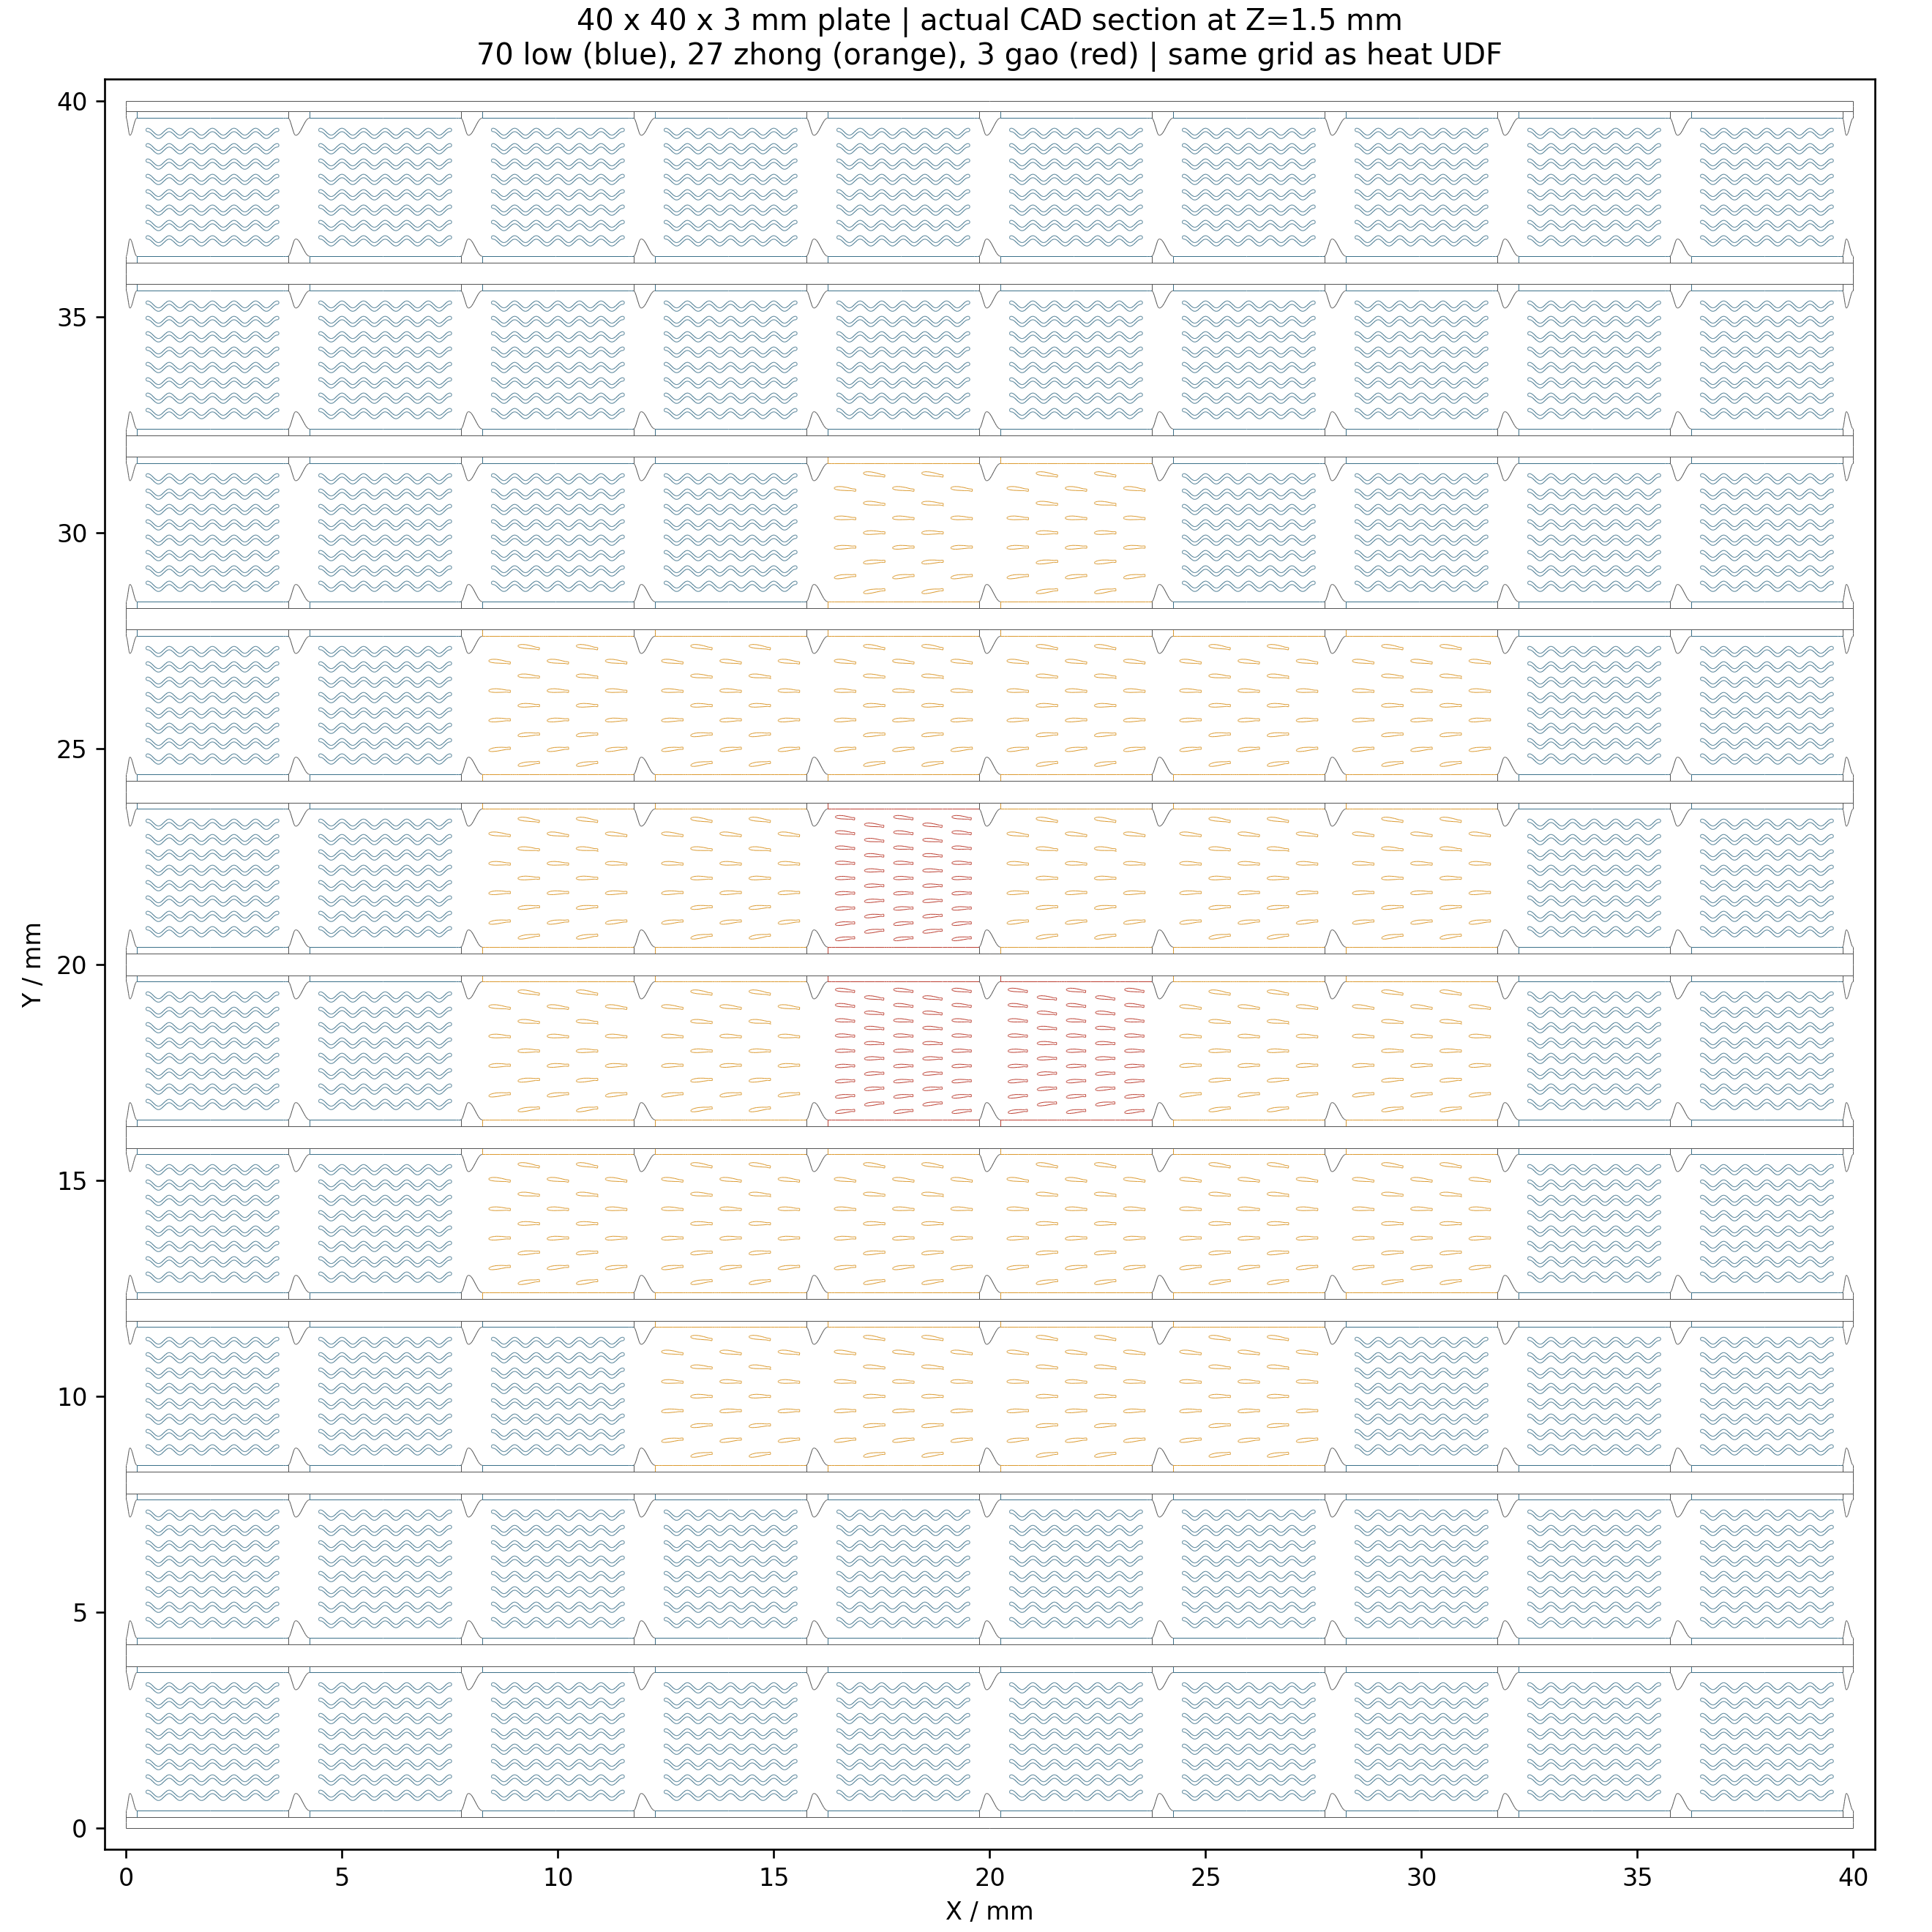
\includegraphics[width=\linewidth,height=88mm,keepaspectratio]{../../figs/midterm_asset_whole_plate.png}
\caption{当前40 mm整板在 z=1.5 mm 的实际 CAD 截面：70个低负荷、27个中负荷、3个高负荷模块。此图为几何与映射核对，不是整板温度场。}\label{fig:05}
\end{subfigure}\hfill
\begin{subfigure}{0.49\linewidth}\centering
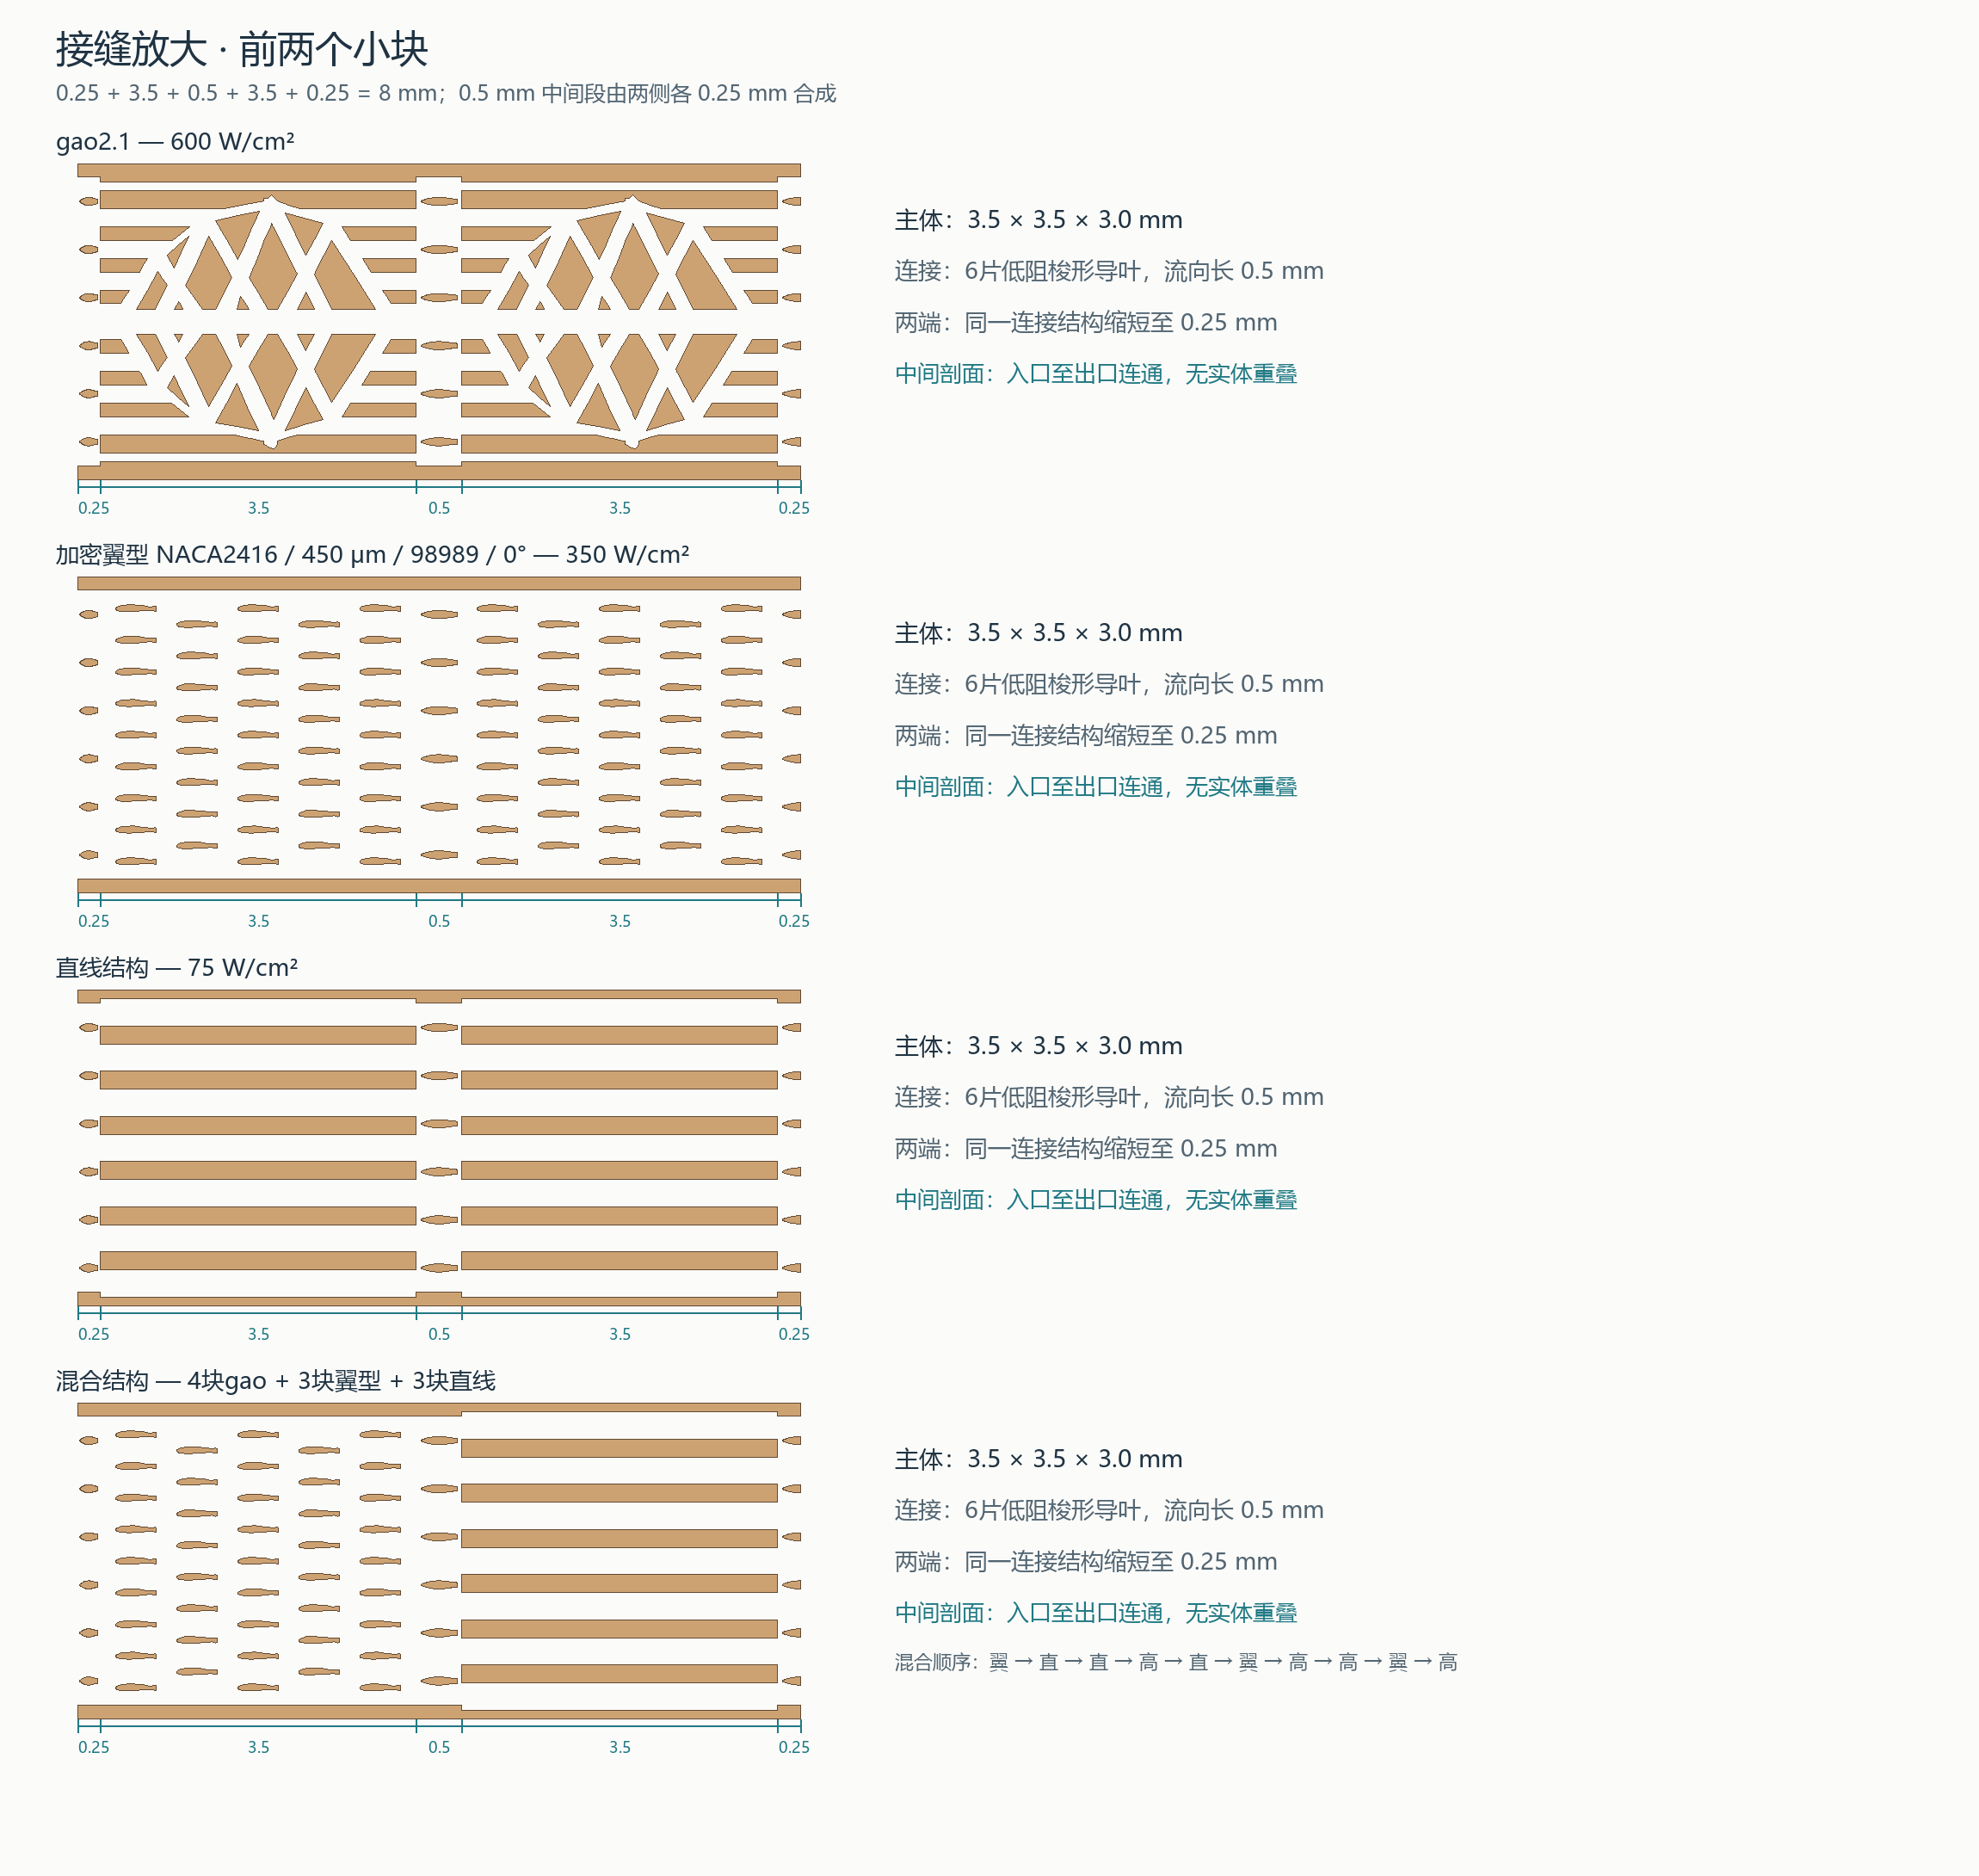
\includegraphics[width=\linewidth,height=88mm,keepaspectratio]{../../figs/midterm_asset_joint_detail.png}
\caption{40 mm条带装配的接缝放大：主体、六片梭形导叶及内部0.5 mm、端部0.25 mm连接。图注热流为后续主体工况配置，未表示条带已经完成求解。}\label{fig:06}
\end{subfigure}
\caption{整板分区与条带接缝的实际几何}
\label{fig:05-06}
\end{figure}
\clearpage
\setcounter{section}{2}
\setcounter{table}{2}
\begin{table}[!htbp]
\centering\small
\caption{三类代表性热负荷工作模式}\label{tab:07}
\begin{tabularx}{\linewidth}{CC}
\toprule
\rowcolor{ydzjlight} 工作模式 & 研究侧重点 \\
\midrule
低热负荷 & 满足温度要求并控制流动代价 \\
高稳定负荷 & 持续热点、局部热阻与连接作用 \\
动态波动负荷 & 响应、恢复和泵阀调控接口 \\
\bottomrule
\end{tabularx}
\end{table}
\clearpage
\setcounter{section}{2}
\setcounter{figure}{1}
\reportfigure{fig:12}{三类代表性负荷与区域结构配置}{../../figs/midterm_concept_fig_12.pdf}{\linewidth}
\clearpage
\setcounter{section}{2}
\setcounter{table}{3}
\begin{table}[!htbp]
\centering\small
\caption{CFD工况与边界条件维护表}\label{tab:03}
\begin{tabularx}{\linewidth}{lYY}
\toprule
\rowcolor{ydzjlight} 设置 & 已读取案例或当前规划 & 待确认范围 \\
\midrule
模型 & 三维、层流、能量方程 & 代表性物性对照已用；新参数范围需复核适用性。 \\
入口 & $2\,\mathrm{m/s}$，$300\,\mathrm K$ & 当前整板规划沿用历史参数；局部最终对照另核。 \\
出口 & 表压0 Pa，回流$302\,\mathrm K$ & 当前整板规划，不能外推至全部历史案例。 \\
固体 & 铜 & — \\
水物性 & REFPROP拟合，280--360 K & 拟合评估压力101325 Pa；记录启用函数版本。 \\
热边界 & 空间三档映射；动态时序另设 & — \\
求解类型 & 物性对照：瞬态；整板规划：稳态 & — \\
数值格式 & 物性对照：SIMPLE，一阶隐式时间格式 & — \\
残差目标 & 物性对照：连续性/速度$10^{-3}$，能量$10^{-6}$ & 每步最多20次内迭代；生产样本准入须另确认。 \\
重力/操作压力 & 代表性案例关闭重力；101325 Pa & — \\
\bottomrule
\end{tabularx}
\end{table}
\clearpage
\setcounter{section}{2}
\setcounter{table}{4}
\begin{table}[!htbp]
\centering\small
\caption{当前物性模型、热源UDF与实现核对}\label{tab:05}
\begin{tabularx}{\linewidth}{lYY}
\toprule
\rowcolor{ydzjlight} 类别 & 已知配置或核对值 & 适用边界与待补项 \\
\midrule
密度 & $996.556916\,\mathrm{kg/m^3}$（300 K） & water\_rp\_density；仅当前拟合版本。 \\
比热 & $4180.636970\,\mathrm{J/(kg\cdot K)}$（300 K） & water\_rp\_cp；焓由相同比热积分。 \\
动力黏度 & $8.537430\times10^{-4}\,\mathrm{Pa\cdot s}$（300 K） & water\_rp\_viscosity。 \\
导热系数 & $0.609500\,\mathrm{W/(m\cdot K)}$（300 K） & water\_rp\_conductivity。 \\
拟合范围 & 280--360 K，101325 Pa & 物性拟合条件；超范围需扩展或更换模型。 \\
实现对照 & 共同0.137 s：加热面最高温差约$3.197\times10^{-6}$ K & 同初场、步长；不是绝对物理精度验证。 \\
静态空间热源 & 75/350/600 W/cm$^2$；70/27/3格 & 整格加热2640 W；主体面积加热2021.25 W。 \\
动态热源 & 已探索随机波动、趋势与峰值 & — \\
\bottomrule
\end{tabularx}
\end{table}
\clearpage
\setcounter{section}{2}
\setcounter{figure}{2}
\begin{figure}[!htbp]\centering
\begin{subfigure}[t]{.49\linewidth}\centering
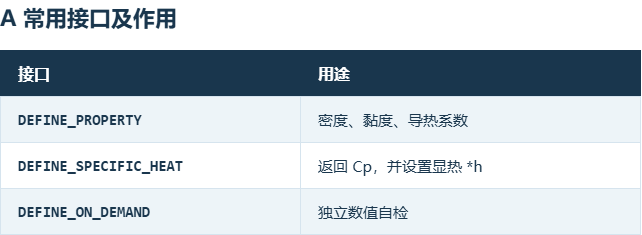
\includegraphics[width=\linewidth]{../../figs/udf_learning_interfaces_a.png}
\caption{常用接口及作用}
\end{subfigure}\hfill
\begin{subfigure}[t]{.49\linewidth}\centering
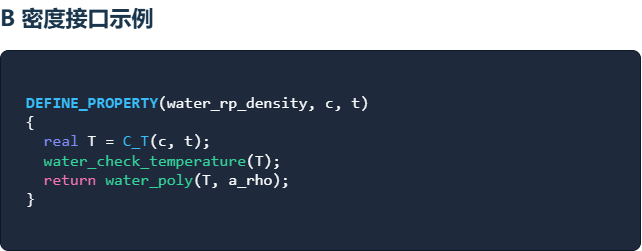
\includegraphics[width=\linewidth]{../../figs/udf_learning_interfaces_b.png}
\caption{密度接口示例}
\end{subfigure}

\vspace{3mm}
\begin{subfigure}[t]{.49\linewidth}\centering
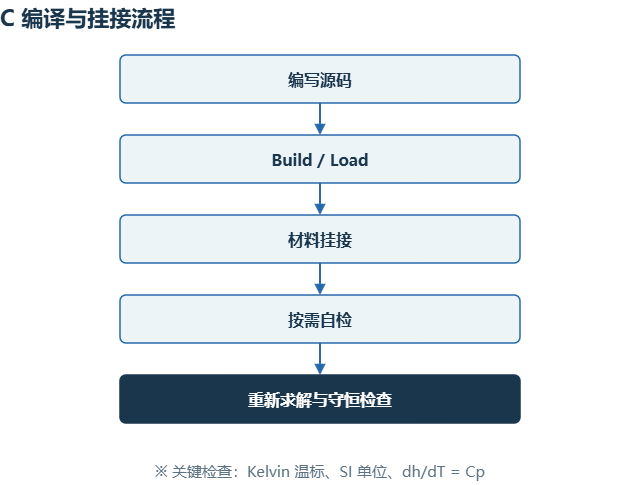
\includegraphics[width=\linewidth]{../../figs/udf_learning_interfaces_c.png}
\caption{编译与挂接流程}
\end{subfigure}\hfill
\begin{subfigure}[t]{.49\linewidth}\centering
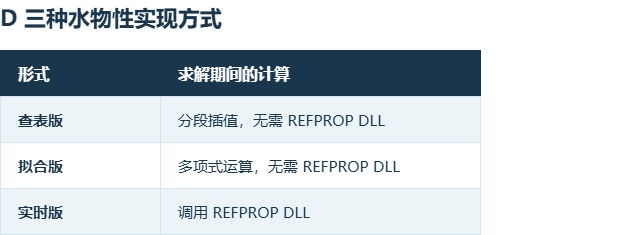
\includegraphics[width=\linewidth]{../../figs/udf_learning_interfaces_d.png}
\caption{三种水物性实现方式}
\end{subfigure}
\caption{水物性 UDF 的温度输入、函数接口、材料挂接与自检流程；正式修改和核验属于本阶段工作。}\label{fig:udf-interface}
\end{figure}
\clearpage
\setcounter{section}{2}
\setcounter{figure}{3}
\reportfigure{fig:11}{数值仿真自动化与样本质量检查流程}{../../figs/midterm_concept_fig_11.pdf}{\linewidth}
\clearpage
\setcounter{section}{2}
\setcounter{table}{5}
\begin{table}[!htbp]
\centering\small
\caption{热工与流动性能指标定义及维护模板}\label{tab:06}
\begin{tabularx}{\linewidth}{CC}
\toprule
\rowcolor{ydzjlight} 指标 & 统计定义 \\
\midrule
$T_{w,\max}$ & 指定受热面最高温度/K \\
$\overline T_{w,A}$ & 受热面面积平均/K \\
$\Delta T_A,\sigma_{T,A}$ & 温度极差与面积标准差/K \\
$R_{\theta,\max}$ & 最高温升/输入功率，K/W \\
$h_{\mathrm{eff}},Nu$ & 界面传热与声明流体参考温度 \\
$\Delta p_s$ & 进出口面积平均静压差/Pa \\
$P_h,P_e$ & 水力功与泵电功率/W \\
守恒误差 & 质量与能量平衡；瞬态含储存项 \\
\bottomrule
\end{tabularx}
\end{table}
\clearpage
\setcounter{section}{2}
\setcounter{table}{6}
\begin{table}[!htbp]
\centering\small
\caption{可追溯连接装配版本及最终对照参数模板}\label{tab:08}
\begin{tabularx}{\linewidth}{CC}
\toprule
\rowcolor{ydzjlight} 参数 & 当前40 mm条带记录 \\
\midrule
连接型式 & 低阻梭形直导叶 \\
导叶数量 & 6片 \\
内部/端部长 & 0.5/0.25 mm \\
外壳宽/高 & 3.5/3.0 mm \\
通腔宽/高 & 3.2/2.5 mm \\
侧壁/上下壁 & 0.15/0.25 mm \\
基准连接 & — \\
\bottomrule
\end{tabularx}
\end{table}
\clearpage
\setcounter{section}{2}
\setcounter{figure}{4}
\begin{figure}[!htbp]\centering
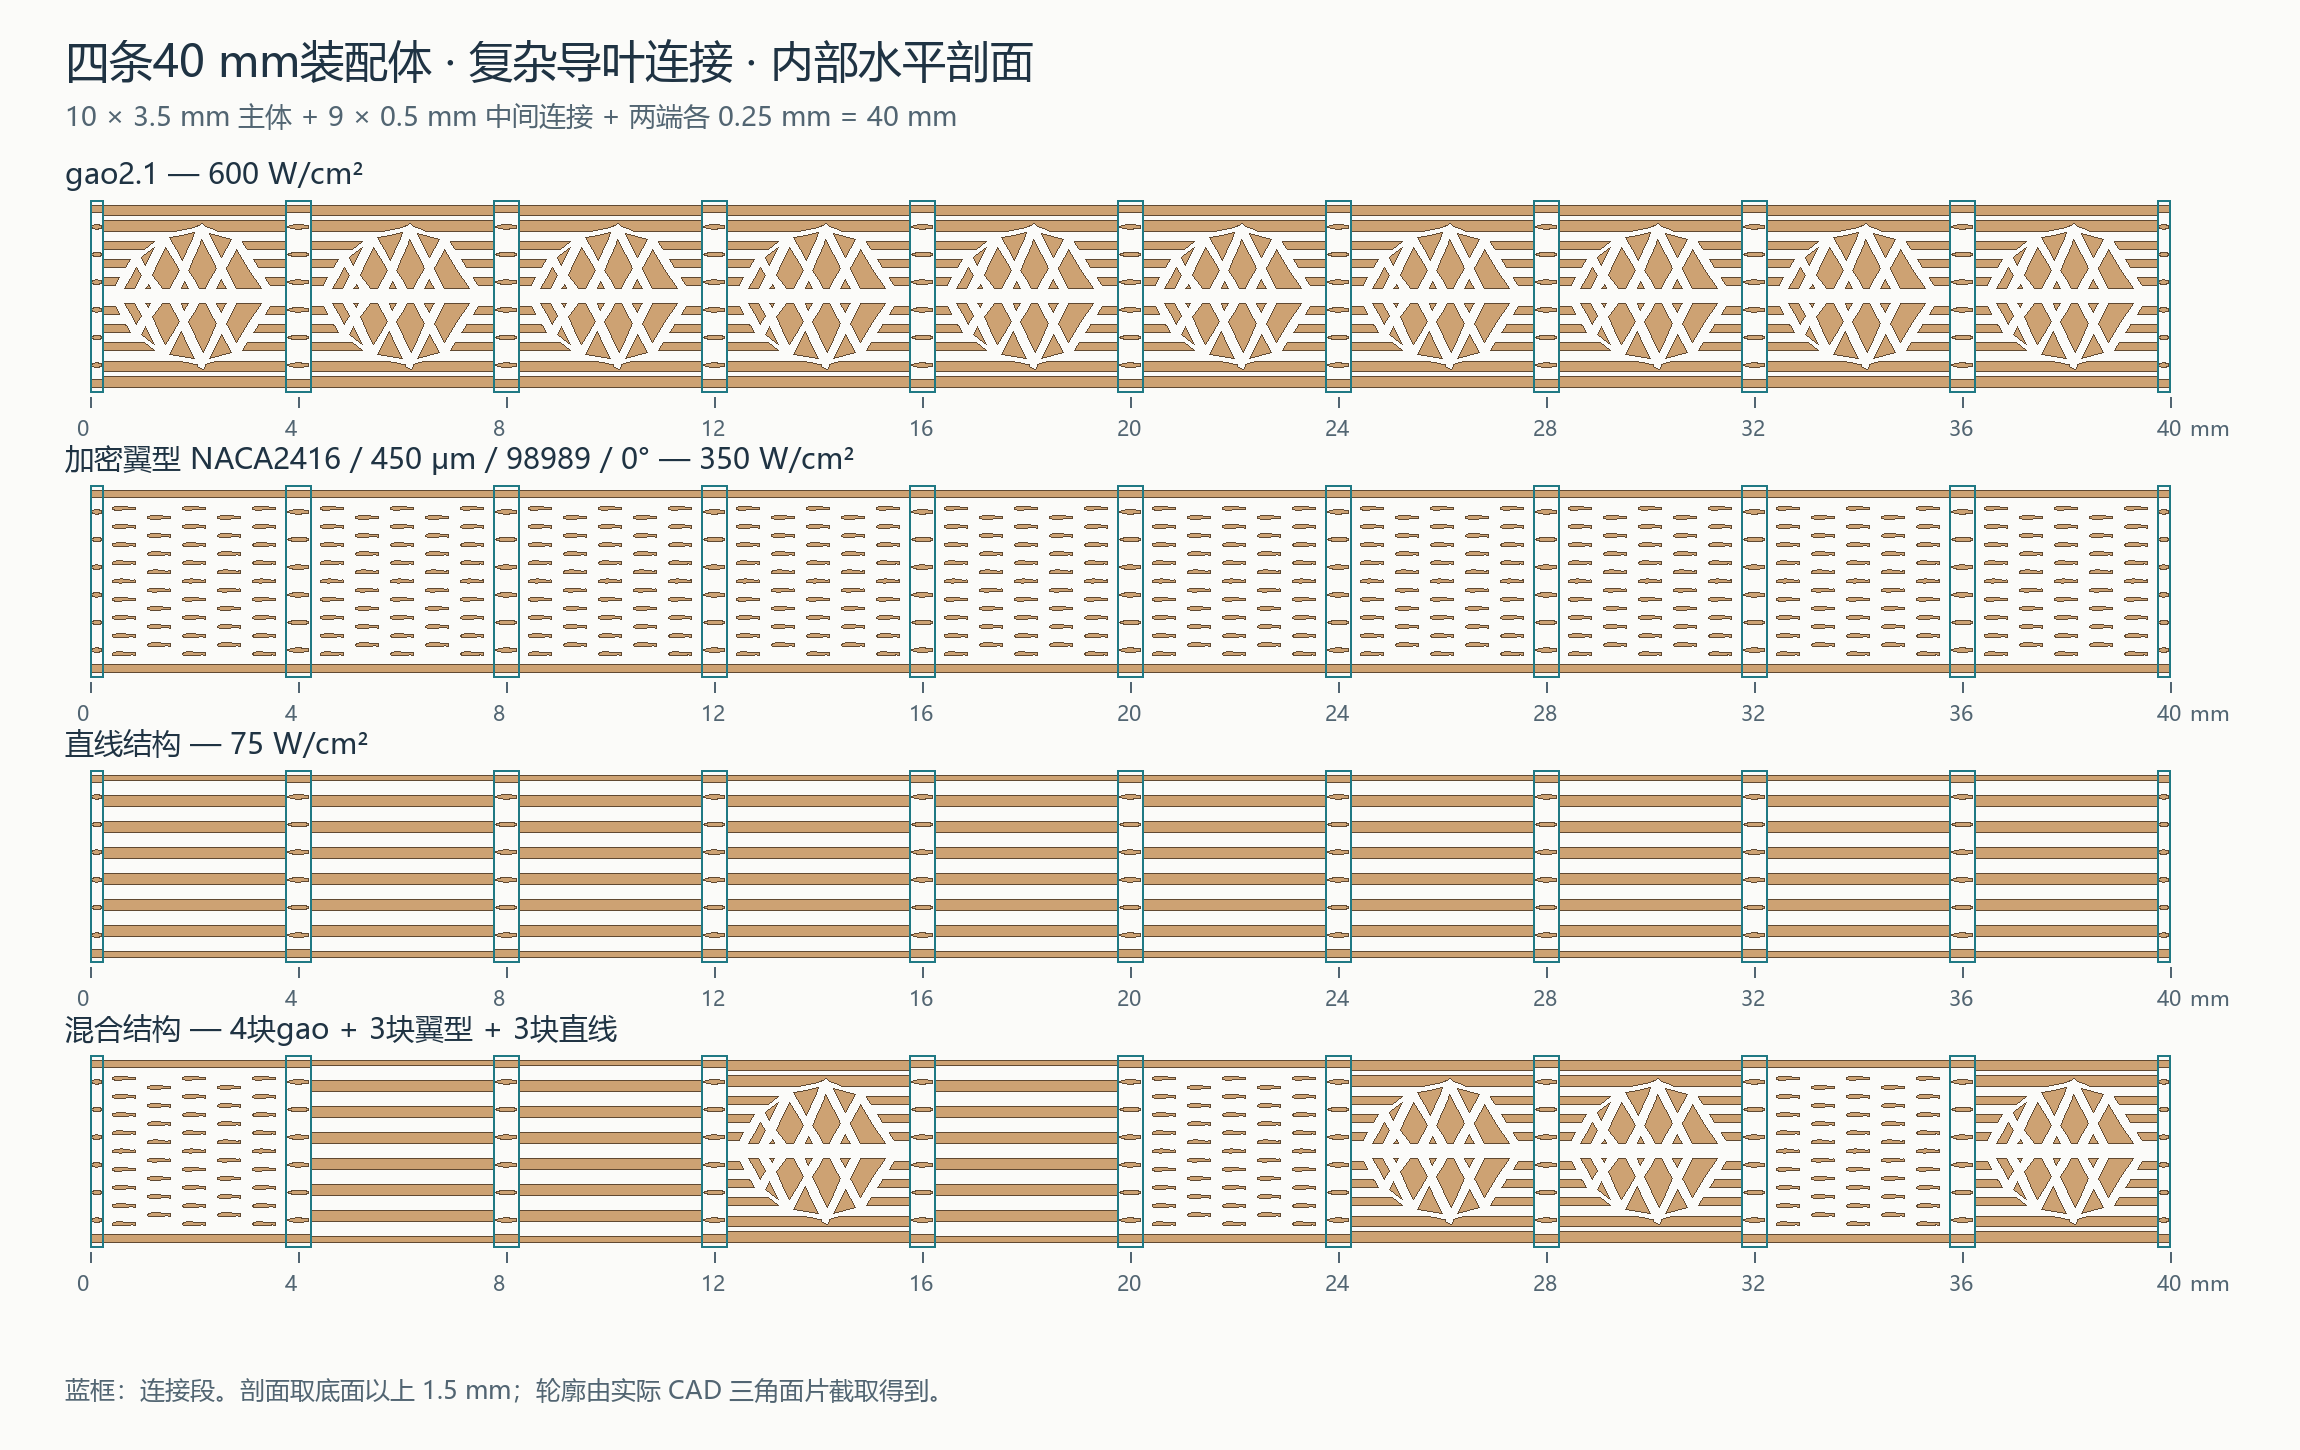
\includegraphics[width=\linewidth,height=125mm,keepaspectratio]{../../figs/midterm_asset_strip_overview.png}
\caption{四条40 mm装配的实际内部截面，包含gao2.1、翼型、直线及混合排列；用于几何准备和接口检查。}\label{fig:13}
\end{figure}
\clearpage
\setcounter{section}{2}
\setcounter{table}{7}
\begin{table}[!htbp]
\centering\small
\caption{连接结构与基准结构的成对性能比较模板}\label{tab:09}
\begin{tabularx}{\linewidth}{CC}
\toprule
\rowcolor{ydzjlight} 指标 & 比较条件 \\
\midrule
$T_{w,\max}$/K & 同热源、同流量或同泵功。 \\
$\overline T_{w,A}$/K & 相同受热面及统计时刻。 \\
$\sigma_{T,A}$/K & 相同区域及面积加权。 \\
$\Delta p$/Pa & 声明静压、总压或能量口径。 \\
$R_\theta$/(K/W) & 声明稳态与总热功率。 \\
$P_h$/W & 流量与系统压力范围一致。 \\
优势与代价 & 仅根据归档数据填入，不编造百分比。 \\
\bottomrule
\end{tabularx}
\par\smallskip\begin{minipage}{\linewidth}\footnotesize 局部单元性能已在前文给出；本表专用于连接段成对验证，不能用不同主体或不同工况的小模型数据代填。\end{minipage}
\end{table}
\clearpage
\setcounter{section}{2}
\setcounter{figure}{5}
\begin{figure}[!htbp]\centering
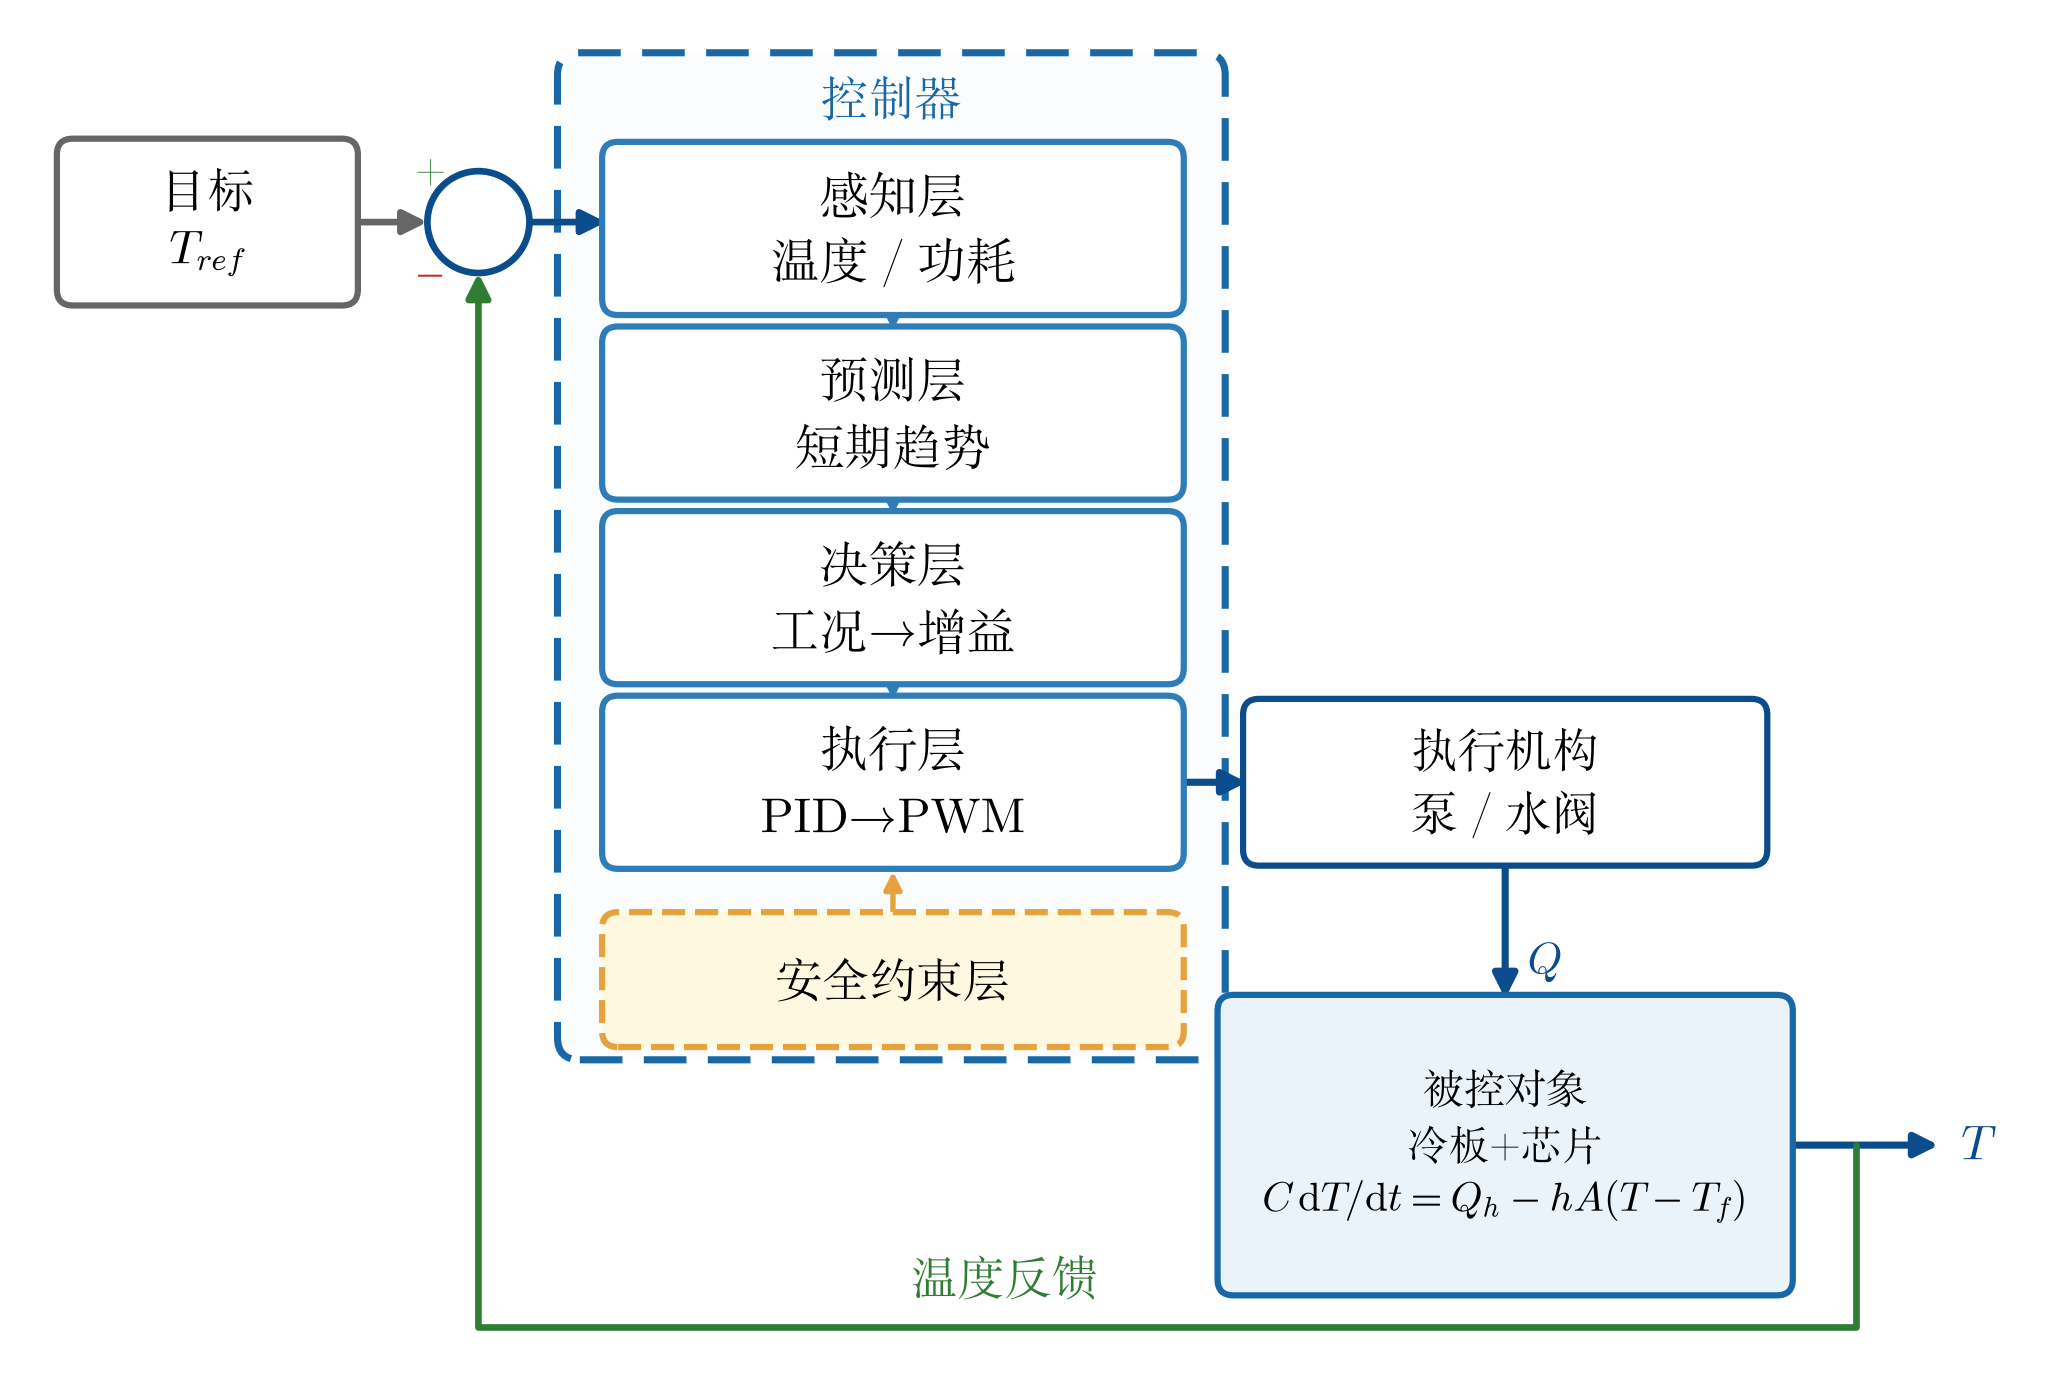
\includegraphics[width=\linewidth]{../../figs/midterm_monthly1_13_控制框架框图.png}
\caption{感知、预测、决策、执行与独立安全约束框架，作为后续系统架构方案。}\label{fig:control-month1}
\end{figure}
\clearpage
\setcounter{section}{2}
\setcounter{figure}{6}
\reportfigure{fig:18}{双泵与行级出口阀门协同控制架构}{../../figs/midterm_concept_fig_18.pdf}{\linewidth}
\clearpage
\setcounter{section}{2}
\setcounter{table}{8}
\begin{table}[!htbp]
\centering\small
\caption{动态系统的输入、状态、测量及控制输出}\label{tab:10}
\begin{tabularx}{\linewidth}{CC}
\toprule
\rowcolor{ydzjlight} 类别 & 候选量与物理意义 \\
\midrule
扰动输入 & $q_i''(t)$、入口温度 \\
热状态 & $T_i,T_{f,i}$，区域与流体温度 \\
水力状态 & $\dot V_i,\Delta p$，行流量与供液压力 \\
测量输出 & 区域最高温、代表点或平均温度 \\
控制输出 & 两泵转速/流量指令、行级出口阀开度 \\
约束 & 温度上限、最小流量、动作速率 \\
\bottomrule
\end{tabularx}
\end{table}
\clearpage
\setcounter{section}{2}
\setcounter{figure}{7}
\reportfigure{fig:21}{由简化数学模型向物理机理融合动态模型的演进}{../../figs/midterm_concept_fig_21.pdf}{\linewidth}
\clearpage
\setcounter{section}{2}
\setcounter{table}{9}
\begin{table}[!htbp]
\centering\small
\caption{代理模型候选输入、输出与数据标识}\label{tab:12}
\begin{tabularx}{\linewidth}{CC}
\toprule
\rowcolor{ydzjlight} 类别 & 候选内容 \\
\midrule
几何输入 & 翼型、弦长、迎角、间距、柱高 \\
流动输入 & 入口速度或Re、入口温度 \\
热边界输入 & 热流等级、空间类别、必要时间参数 \\
物理特征 & Re、Pr、Pe、几何比值、简化基线 \\
温度输出 & 受热面最高温、出口混合温度 \\
性能输出 & 压降、热阻或Nu \\
元数据 & 几何ID、网格、物性、守恒、计时 \\
\bottomrule
\end{tabularx}
\end{table}
\clearpage
\setcounter{section}{2}
\setcounter{figure}{8}
\reportfigure{fig:24}{高保真CFD样本生成与数据集划分流程}{../../figs/midterm_concept_fig_24.pdf}{\linewidth}
\clearpage
\setcounter{section}{2}
\setcounter{figure}{9}
\reportfigure{fig:25}{物理推导与物理机器学习的双路径框架}{../../figs/midterm_concept_fig_25.pdf}{\linewidth}
\clearpage
\setcounter{section}{2}
\setcounter{table}{10}
\begin{table}[!htbp]
\centering\small
\caption{拟比较代理模型算法与物理融合路径}\label{tab:13}
\begin{tabularx}{\linewidth}{CC}
\toprule
\rowcolor{ydzjlight} 模型路线 & 方法与比较目的 \\
\midrule
基础回归 & XGBoost等；建立无额外物理信息基线 \\
物理特征增强 & 加入无量纲数与可计算机理特征 \\
物理基线+残差 & 学习简化物理模型的剩余偏差 \\
可微约束模型 & 数据项与守恒/边界约束联合训练 \\
简单参考模型 & 线性/低阶回归或可验证关联式 \\
\bottomrule
\end{tabularx}
\par\smallskip\begin{minipage}{\linewidth}\footnotesize 所有算法结果均待产生；不将技术路线写为训练完成。方程约束网络不等同于对XGBoost直接加入PDE自动微分残差。\end{minipage}
\end{table}
\clearpage
\setcounter{section}{2}
\setcounter{figure}{10}
\reportfigure{fig:26}{物理融合代理模型架构与预测任务}{../../figs/midterm_concept_fig_26.pdf}{\linewidth}
\clearpage
\setcounter{section}{3}
\setcounter{table}{0}
\begin{table}[!htbp]
		\centering
		\caption{三种流道的复现情况}
		\label{m1:tab:repro}
		\begin{tabularx}{\textwidth}{@{}Y Y Y@{}}
			\toprule
\rowcolor{ydzjlight} 流道形态 & 复现关注内容 & 结果 \\
			\midrule
			方形微通道 & 方形流路及中心扰动结构的影响 & 已完成，趋势与论文一致 \\
			六边形微通道 & 六边形布局及局部流动组织 & 已完成，趋势与论文一致 \\
			圆形微通道 & 环形流路及流体分配的影响 & 已完成，趋势与论文一致 \\

			\bottomrule
		\end{tabularx}
	\end{table}
\clearpage
\setcounter{section}{3}
\setcounter{figure}{0}
\begin{figure}[!htbp]\centering
{\small\heiti 方形微通道}\par\vspace{1pt}
\begin{subfigure}{.235\linewidth}\centering
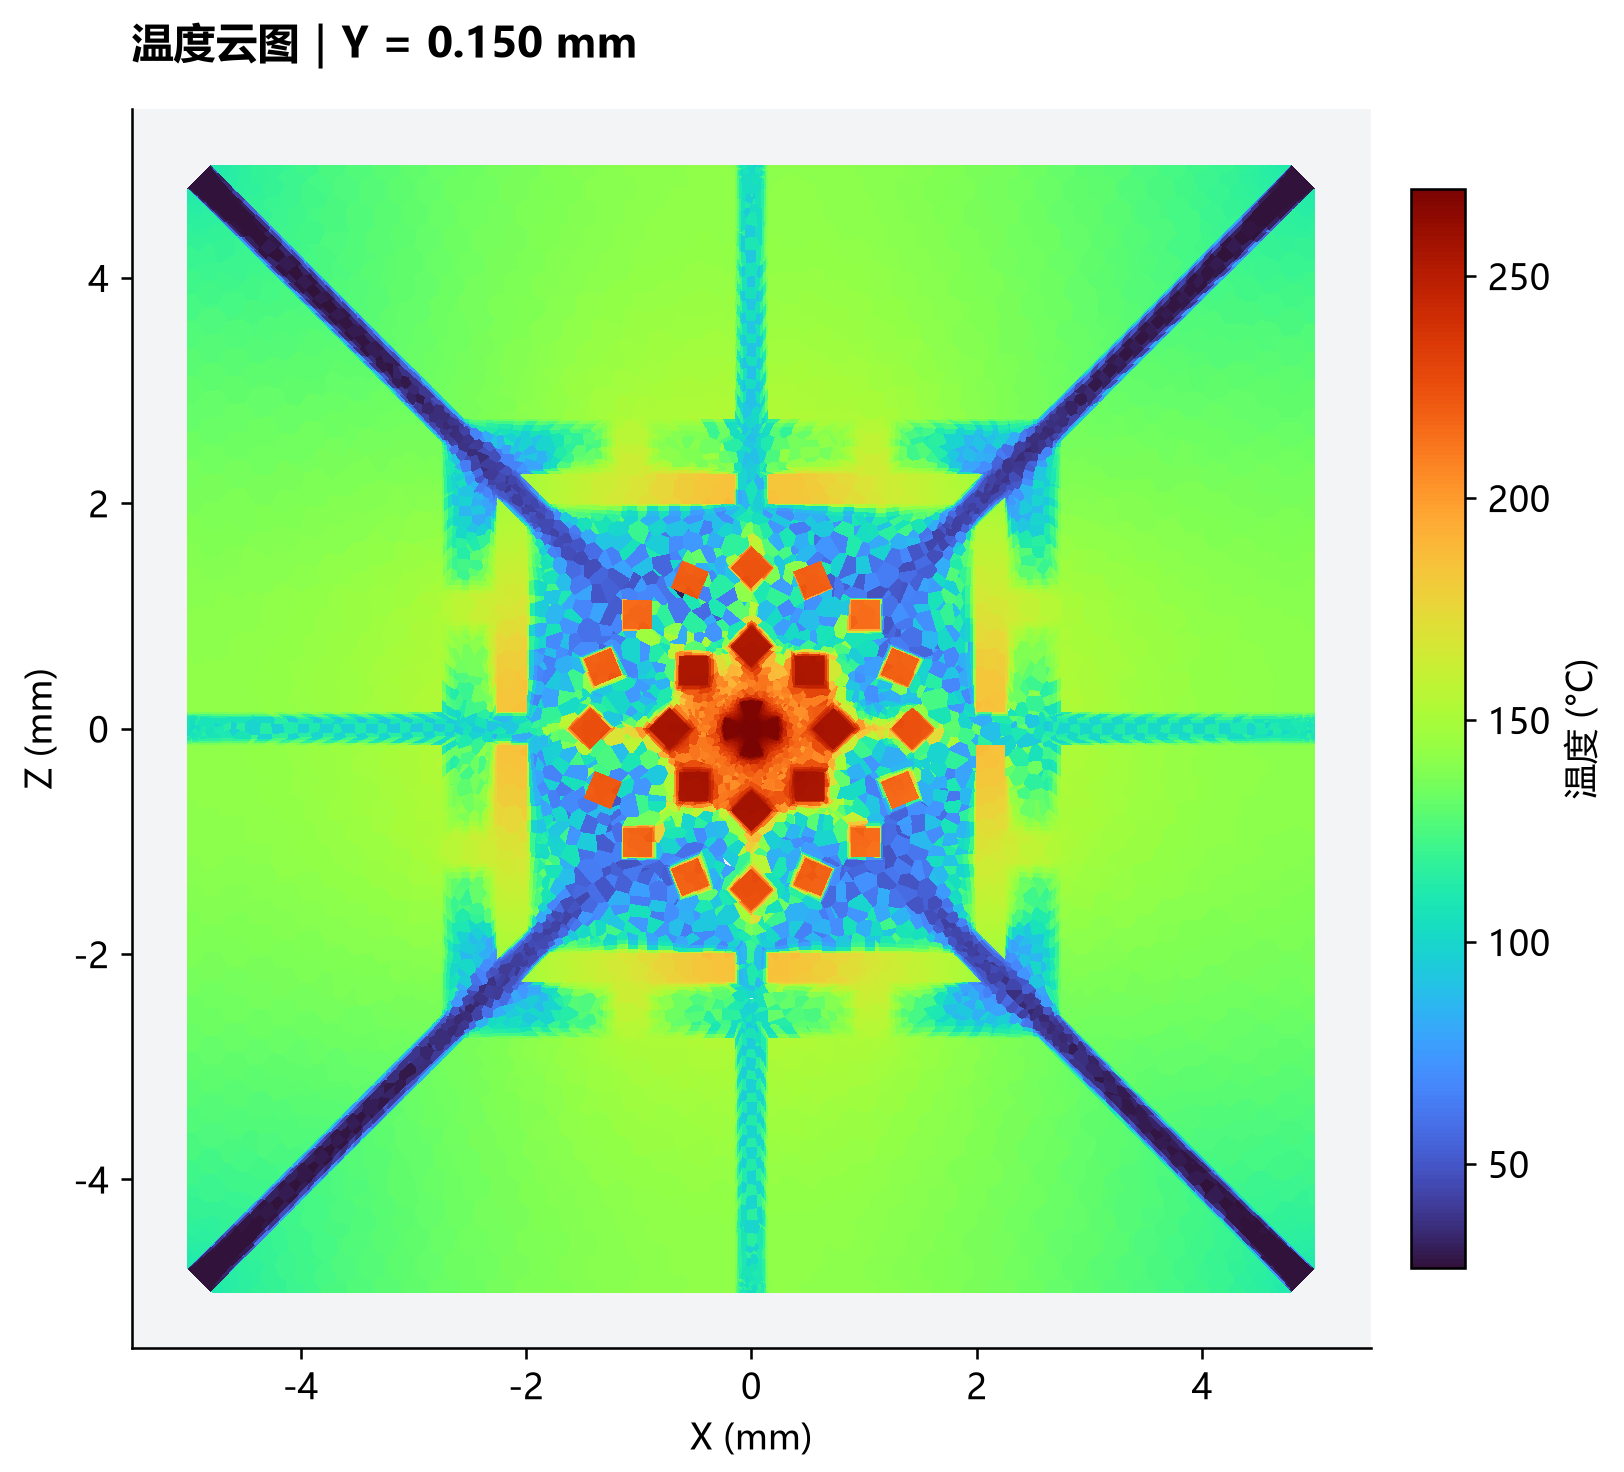
\includegraphics[width=\linewidth]{../../figs/midterm_monthly1_01_temperature_midplane.png}
\caption{水侧温度}\end{subfigure}\hfill
\begin{subfigure}{.235\linewidth}\centering
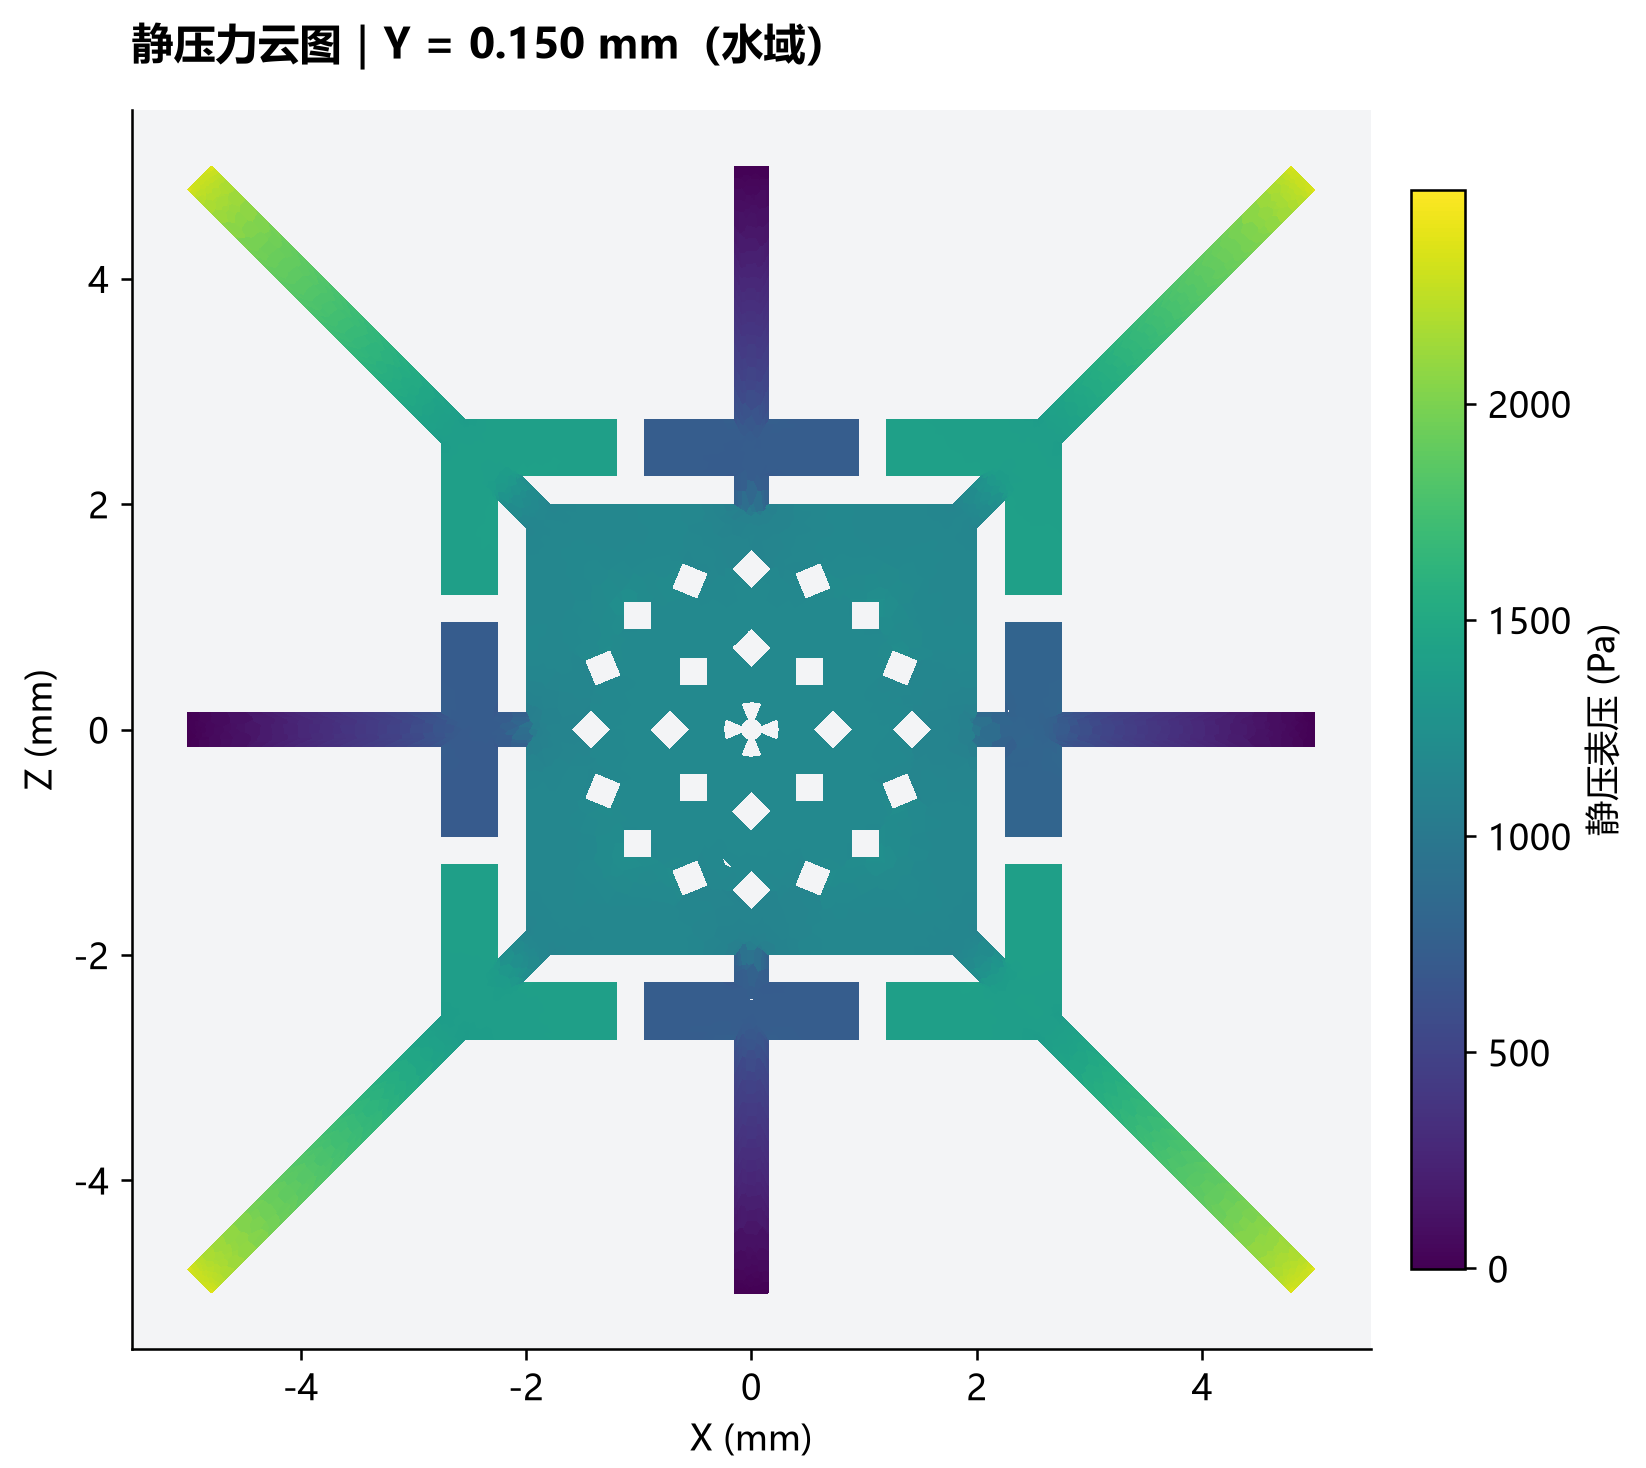
\includegraphics[width=\linewidth]{../../figs/midterm_monthly1_02_pressure_midplane.png}
\caption{水侧表压}\end{subfigure}\hfill
\begin{subfigure}{.235\linewidth}\centering
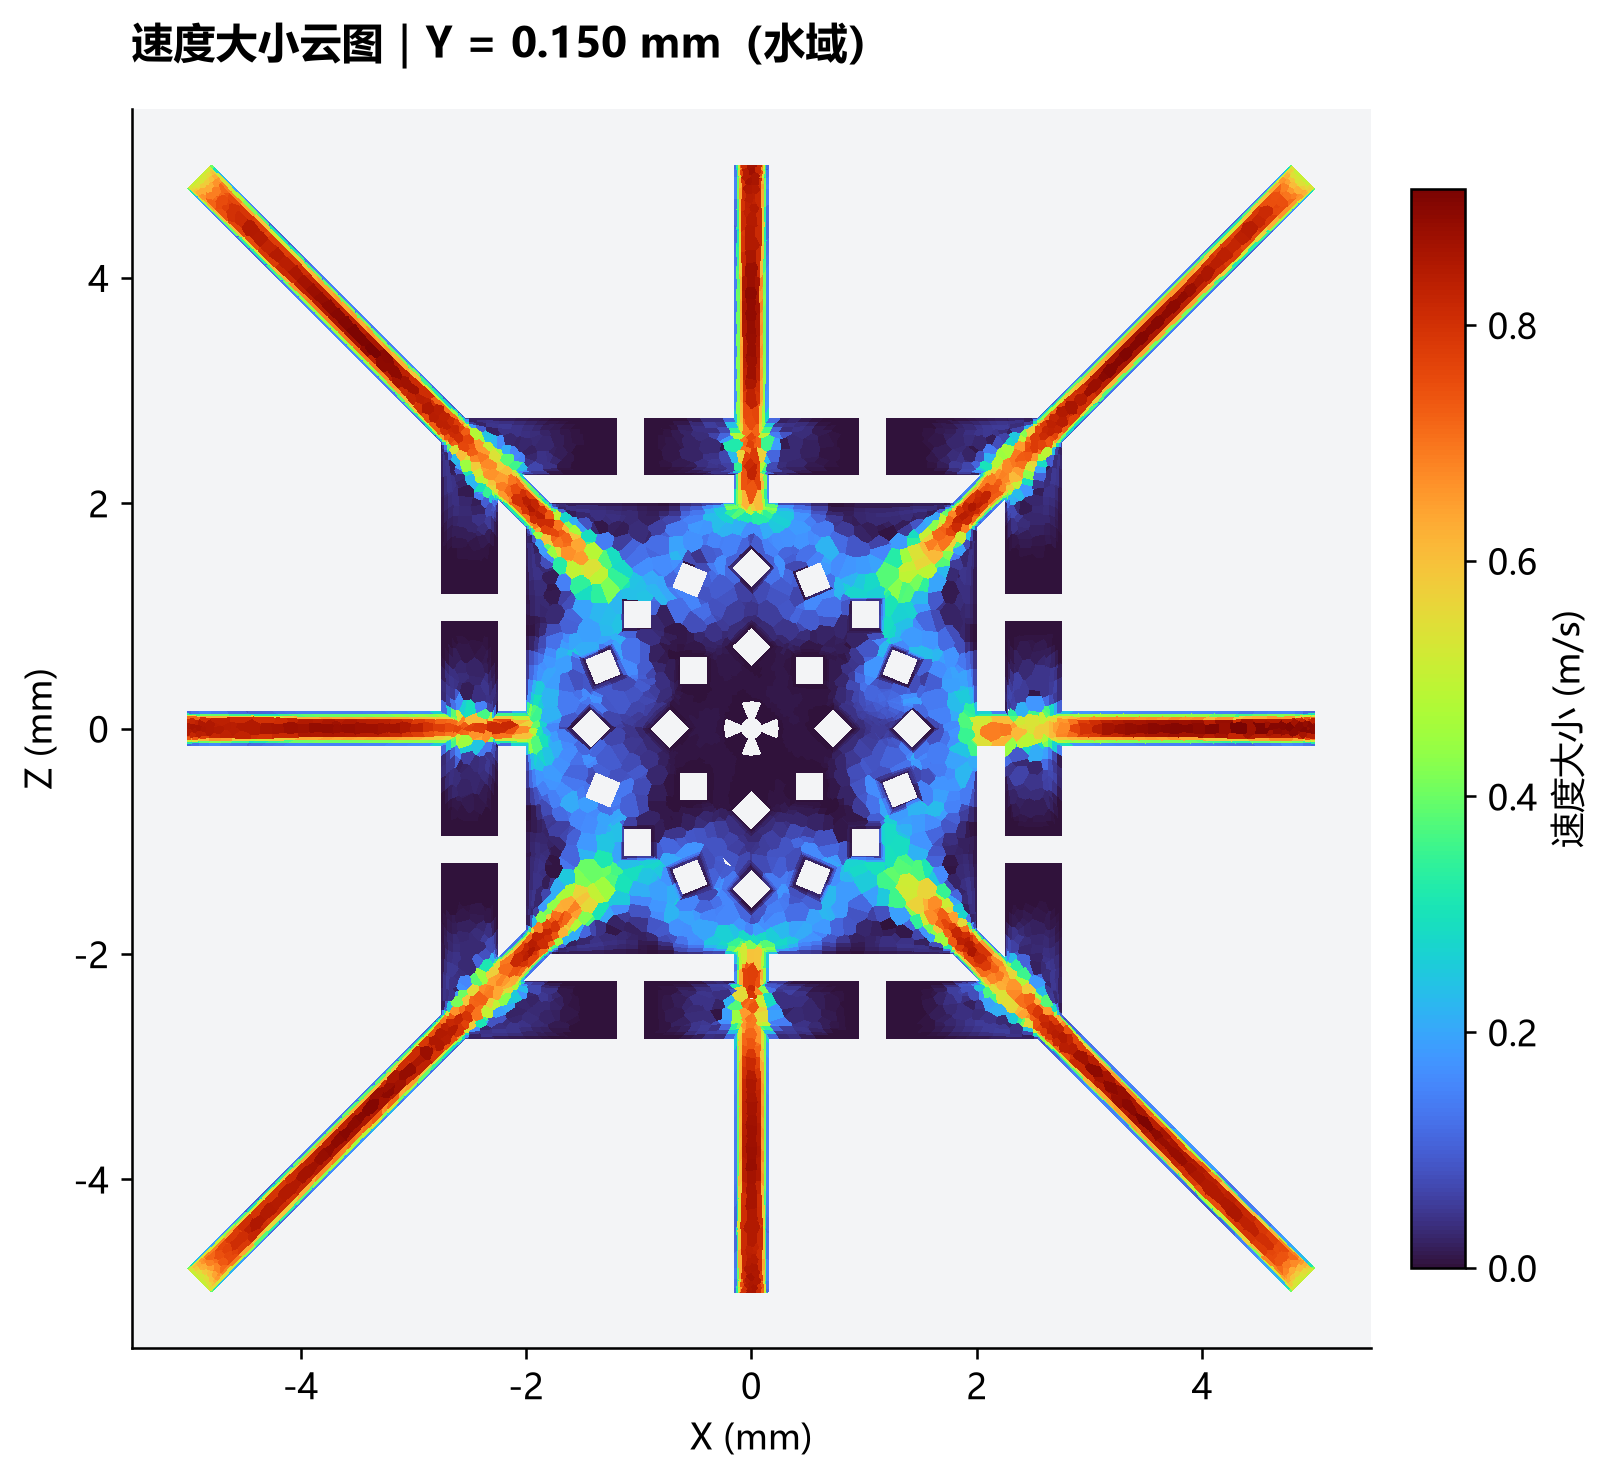
\includegraphics[width=\linewidth]{../../figs/midterm_monthly1_03_speed_midplane.png}
\caption{水侧速度大小}\end{subfigure}\hfill
\begin{subfigure}{.235\linewidth}\centering
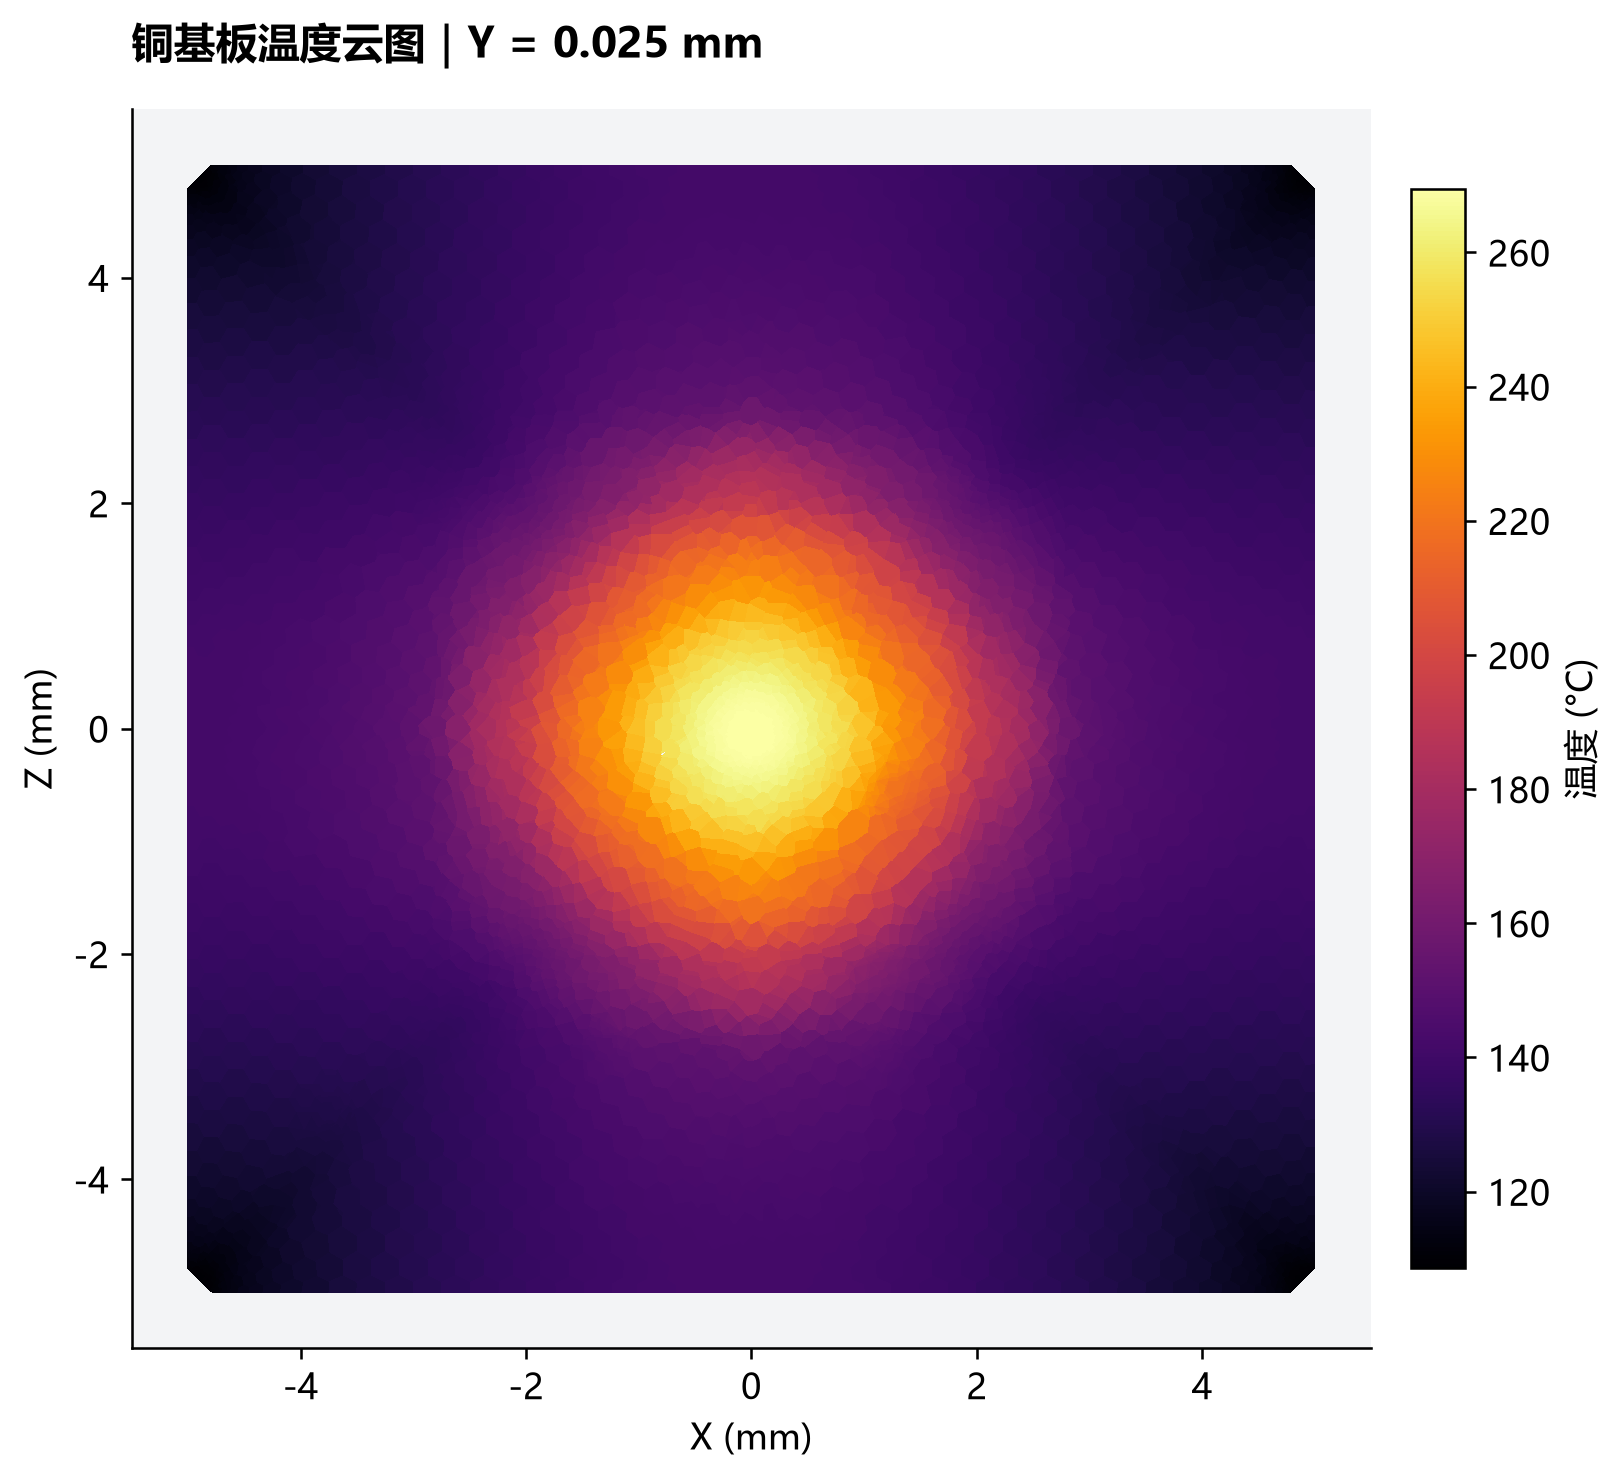
\includegraphics[width=\linewidth]{../../figs/midterm_monthly1_04_copper_base_temperature.png}
\caption{铜基板温度}\end{subfigure}

\vspace{4pt}
{\small\heiti 六边形微通道}\par\vspace{1pt}
\begin{subfigure}{.235\linewidth}\centering
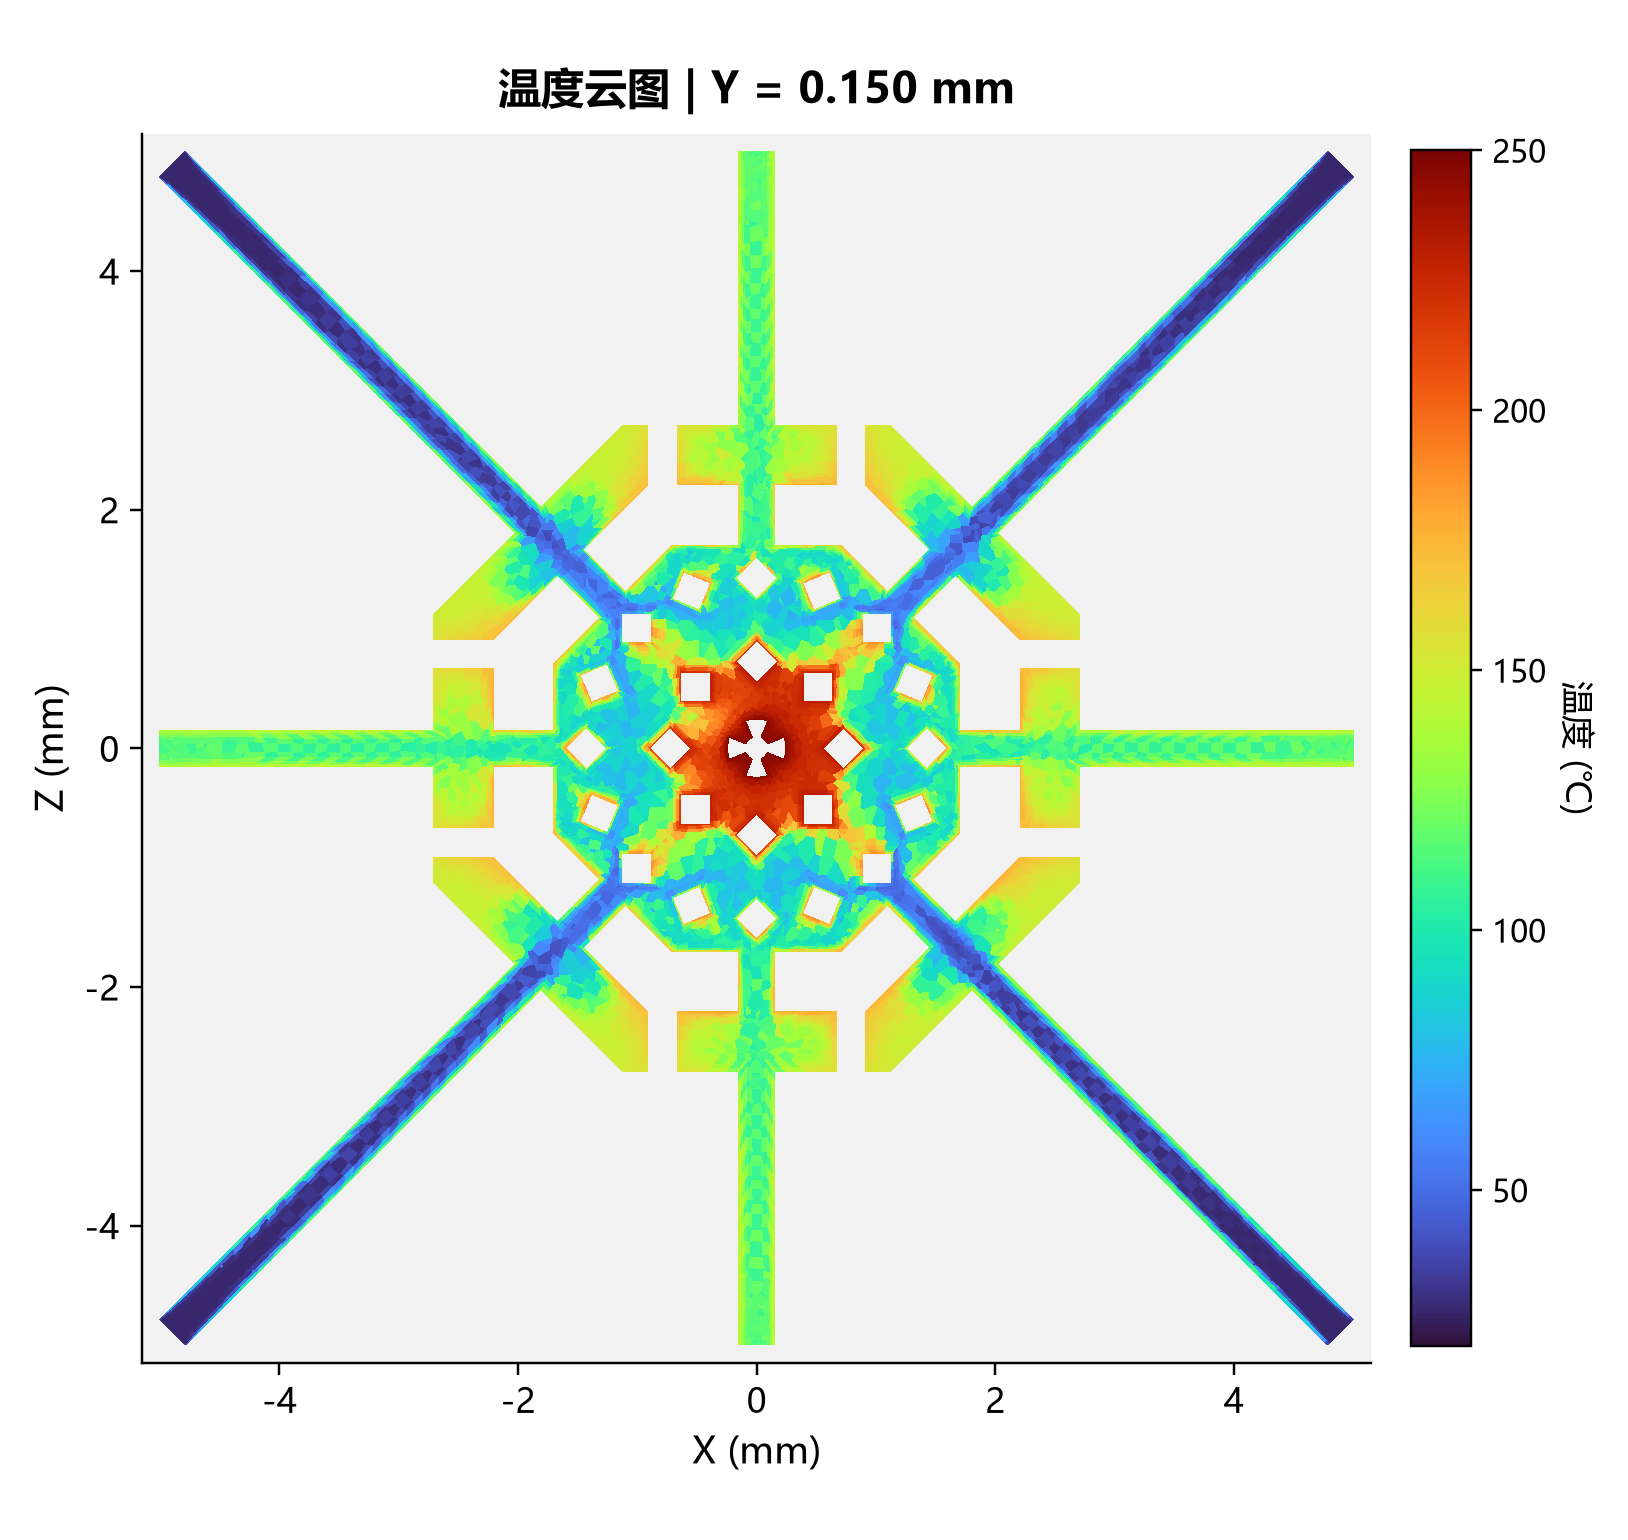
\includegraphics[width=\linewidth]{../../figs/midterm_monthly1_05_temperature_midplane.png}\end{subfigure}\hfill
\begin{subfigure}{.235\linewidth}\centering
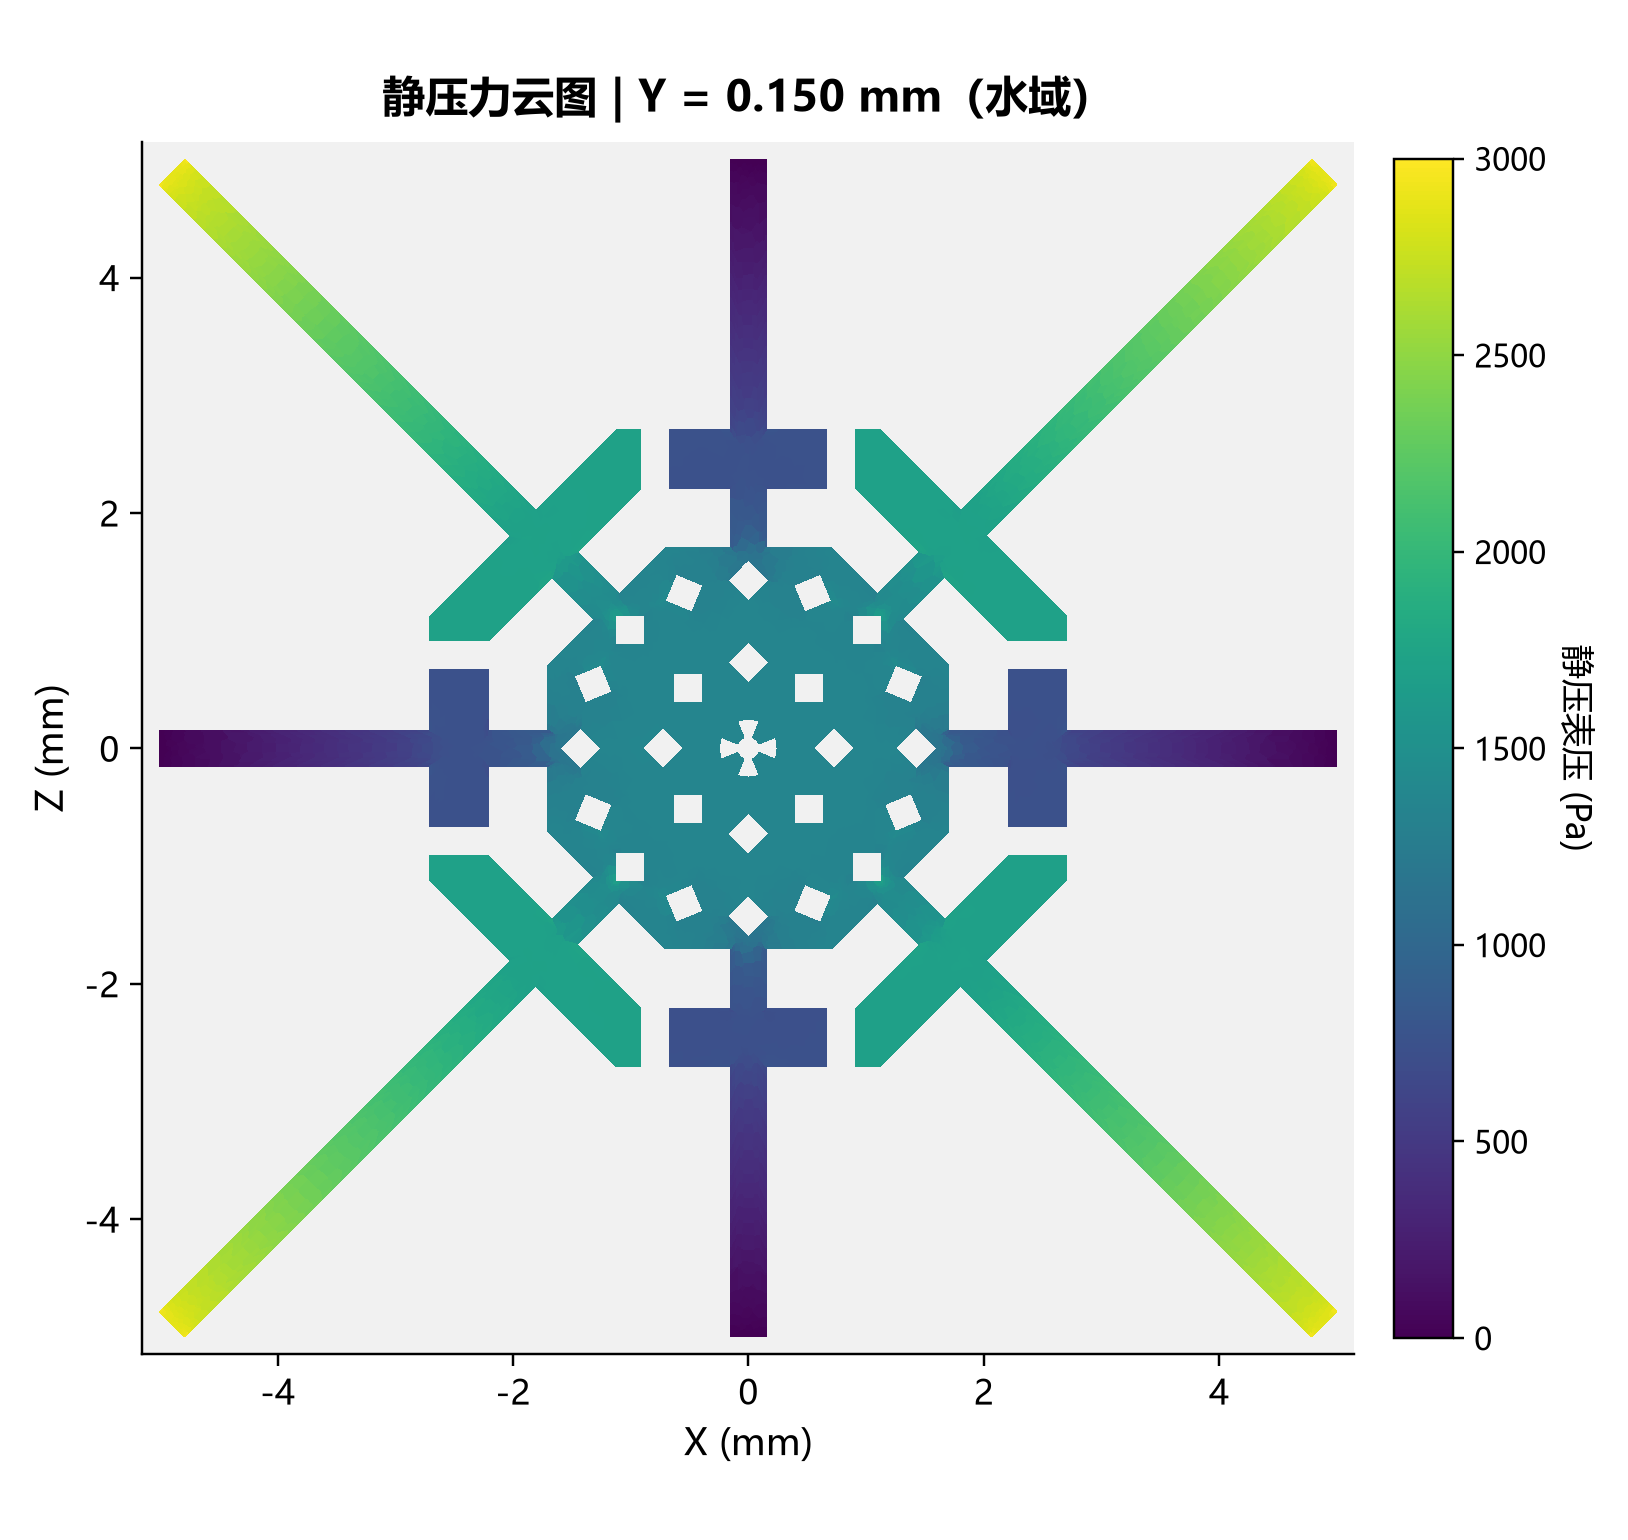
\includegraphics[width=\linewidth]{../../figs/midterm_monthly1_06_pressure_midplane.png}\end{subfigure}\hfill
\begin{subfigure}{.235\linewidth}\centering
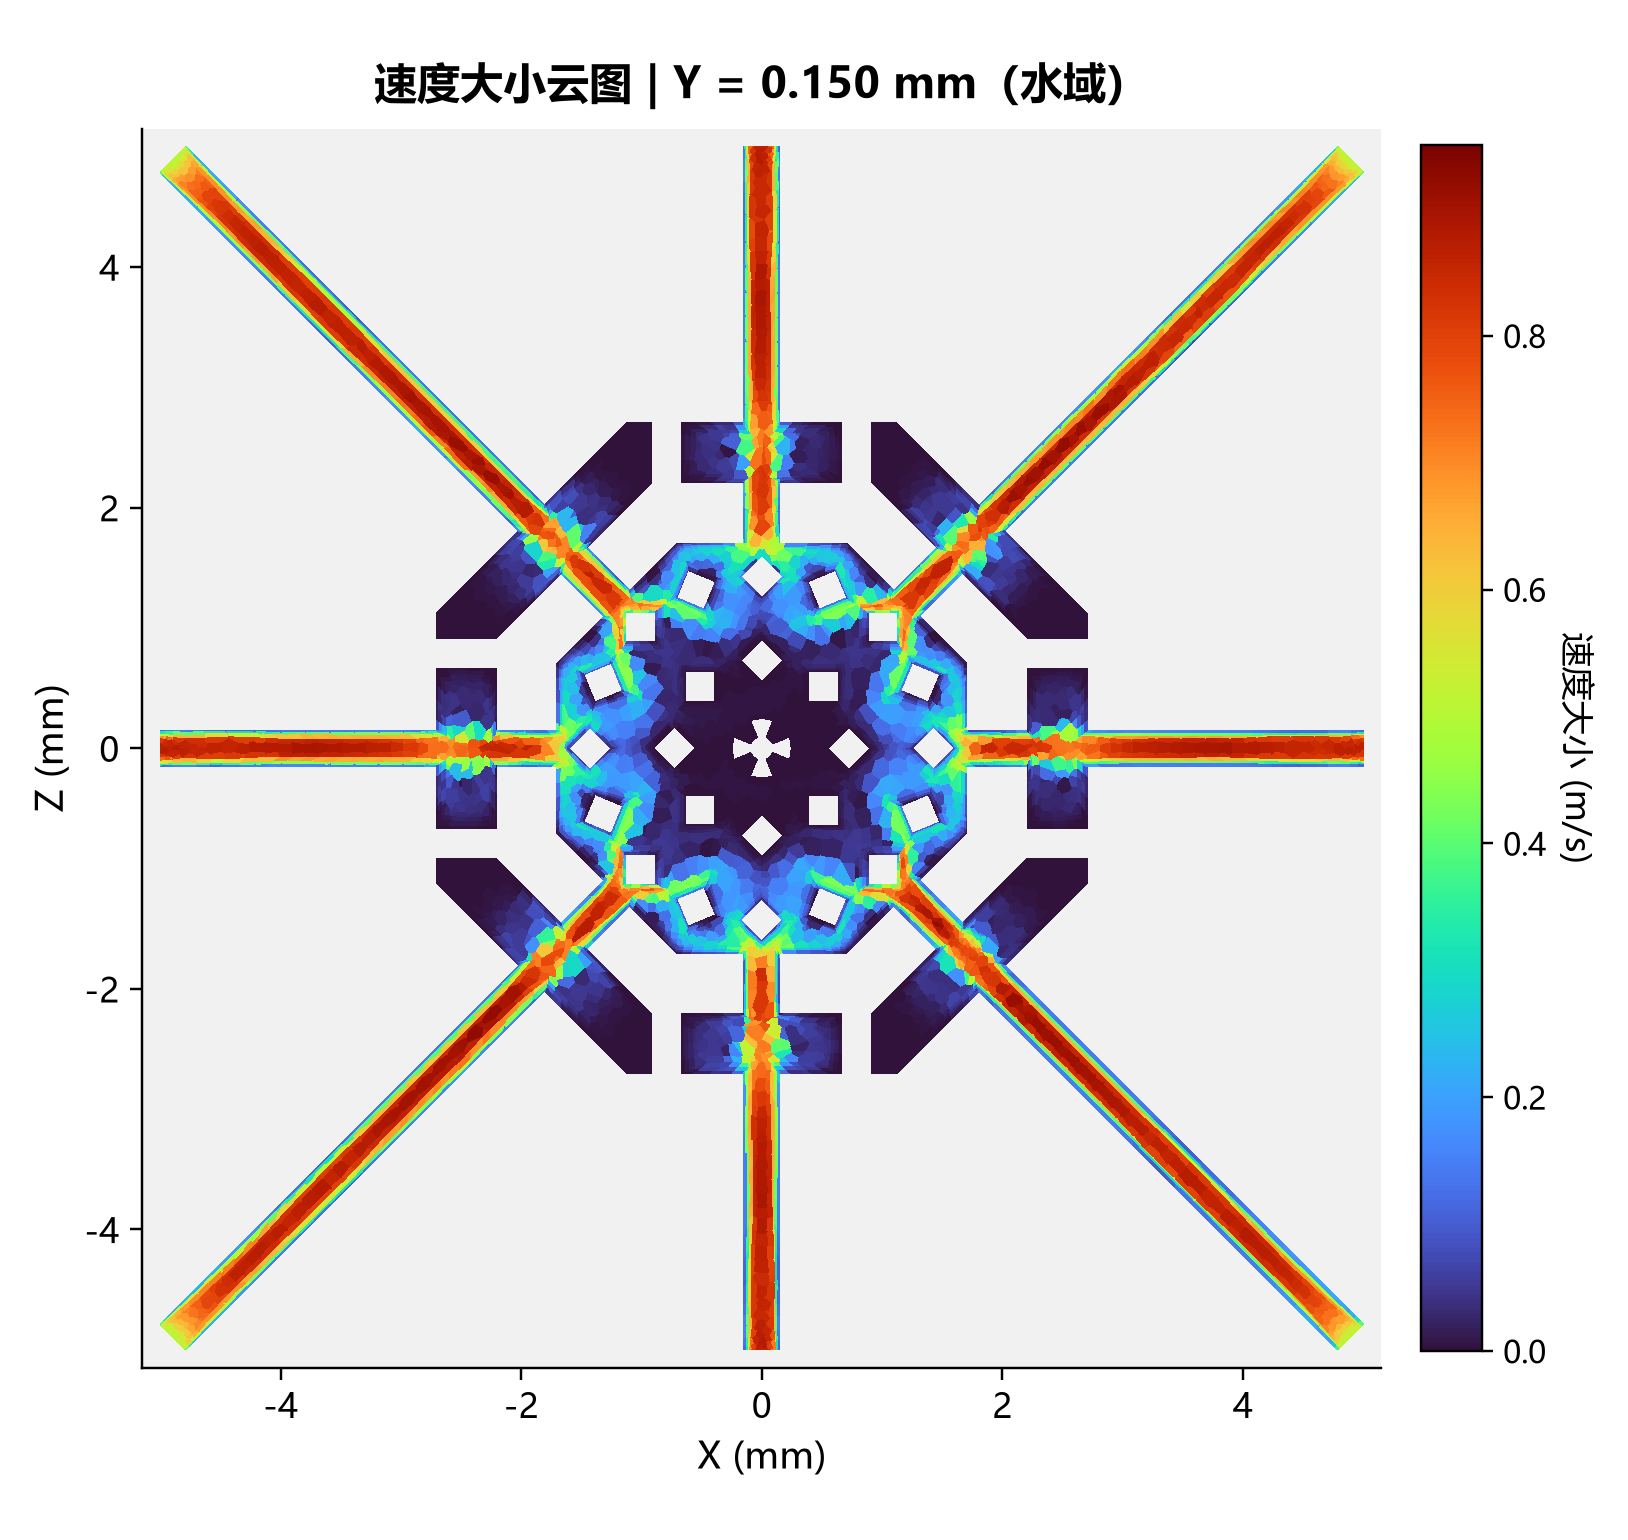
\includegraphics[width=\linewidth]{../../figs/midterm_monthly1_07_speed_midplane.png}\end{subfigure}\hfill
\begin{subfigure}{.235\linewidth}\centering
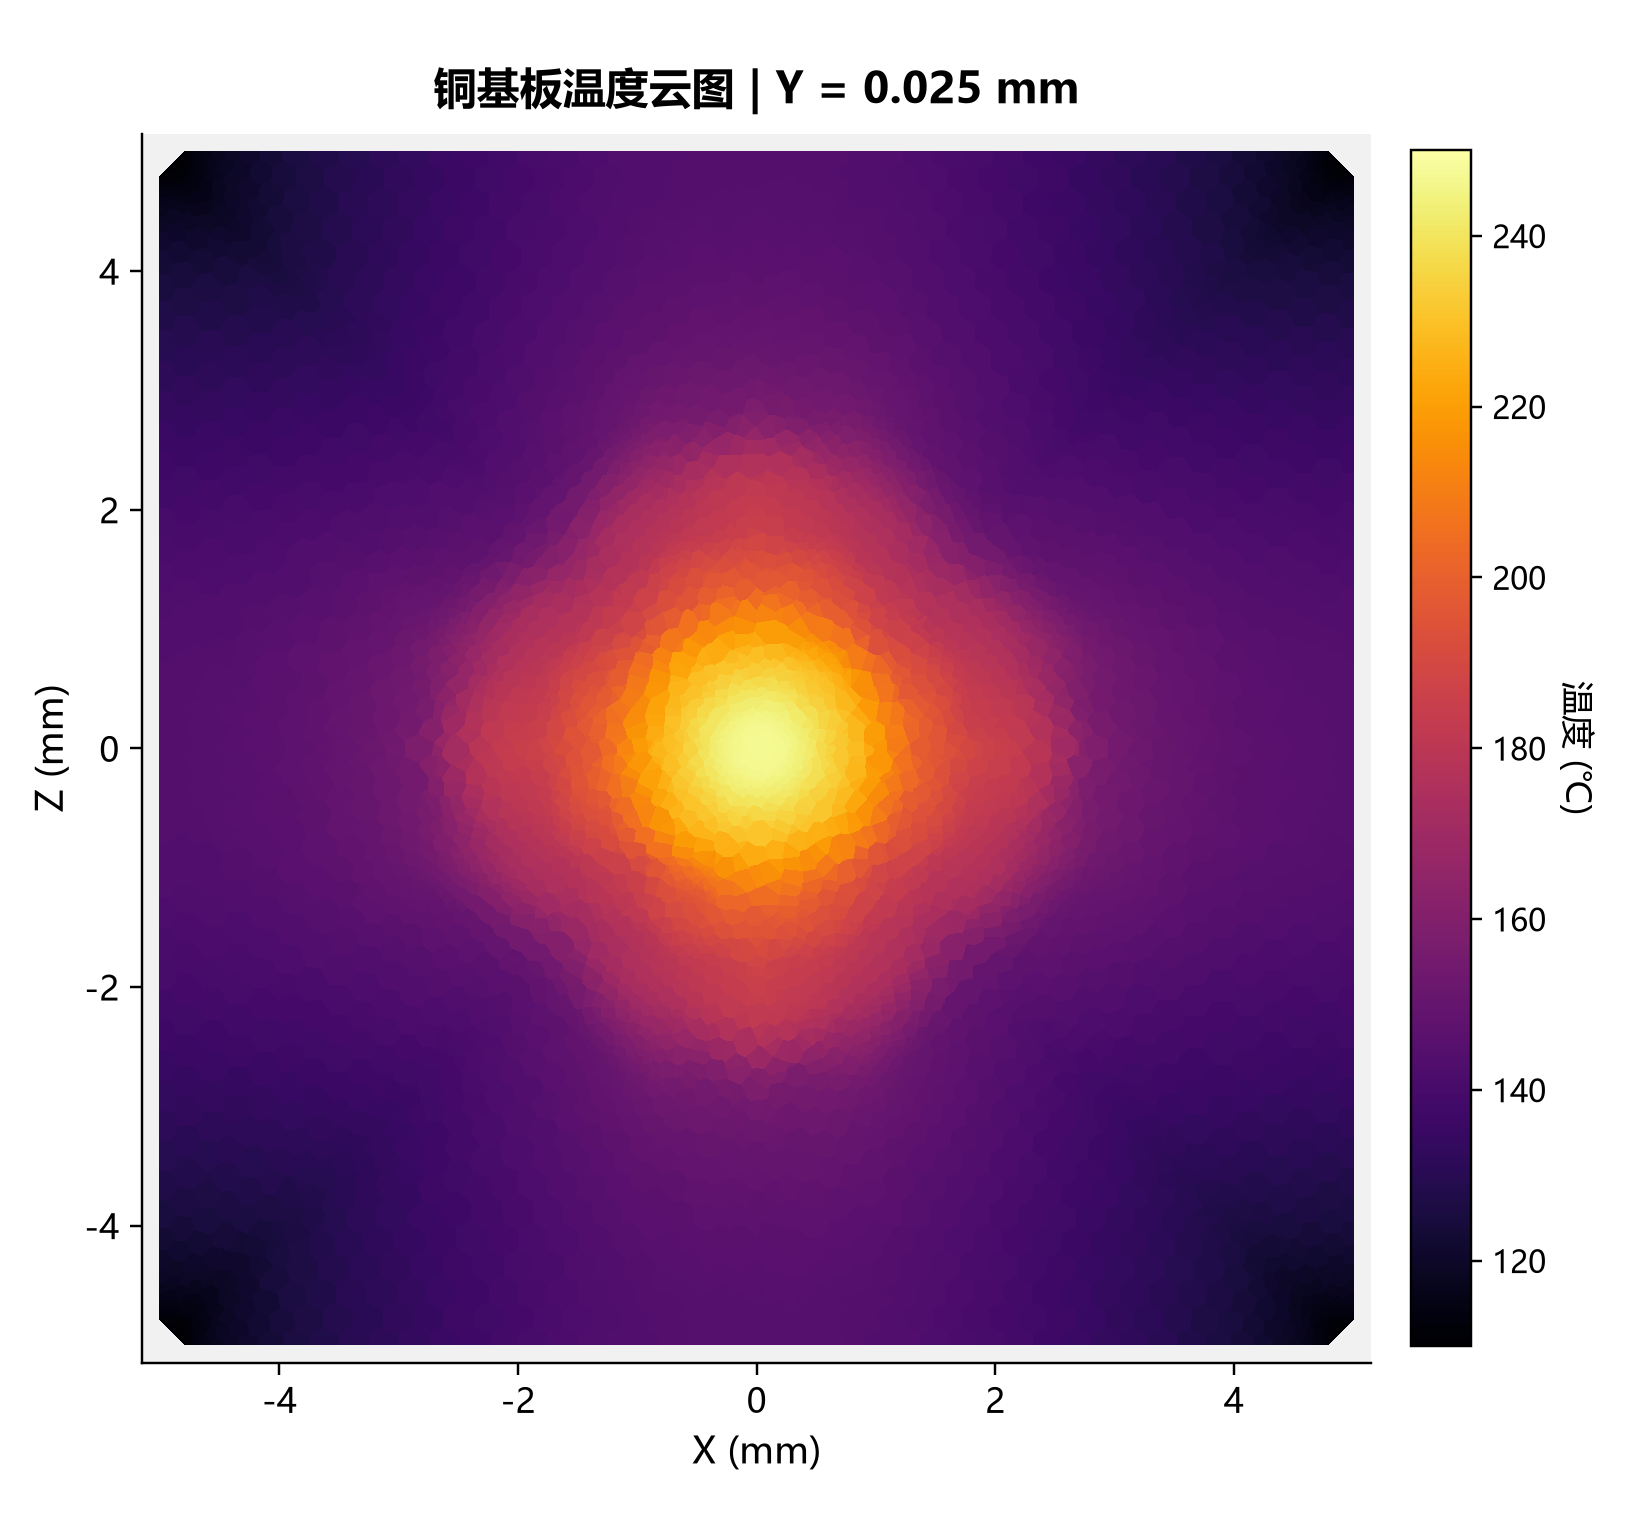
\includegraphics[width=\linewidth]{../../figs/midterm_monthly1_08_copper_base_temperature.png}\end{subfigure}

\vspace{4pt}
{\small\heiti 圆形微通道}\par\vspace{1pt}
\begin{subfigure}{.235\linewidth}\centering
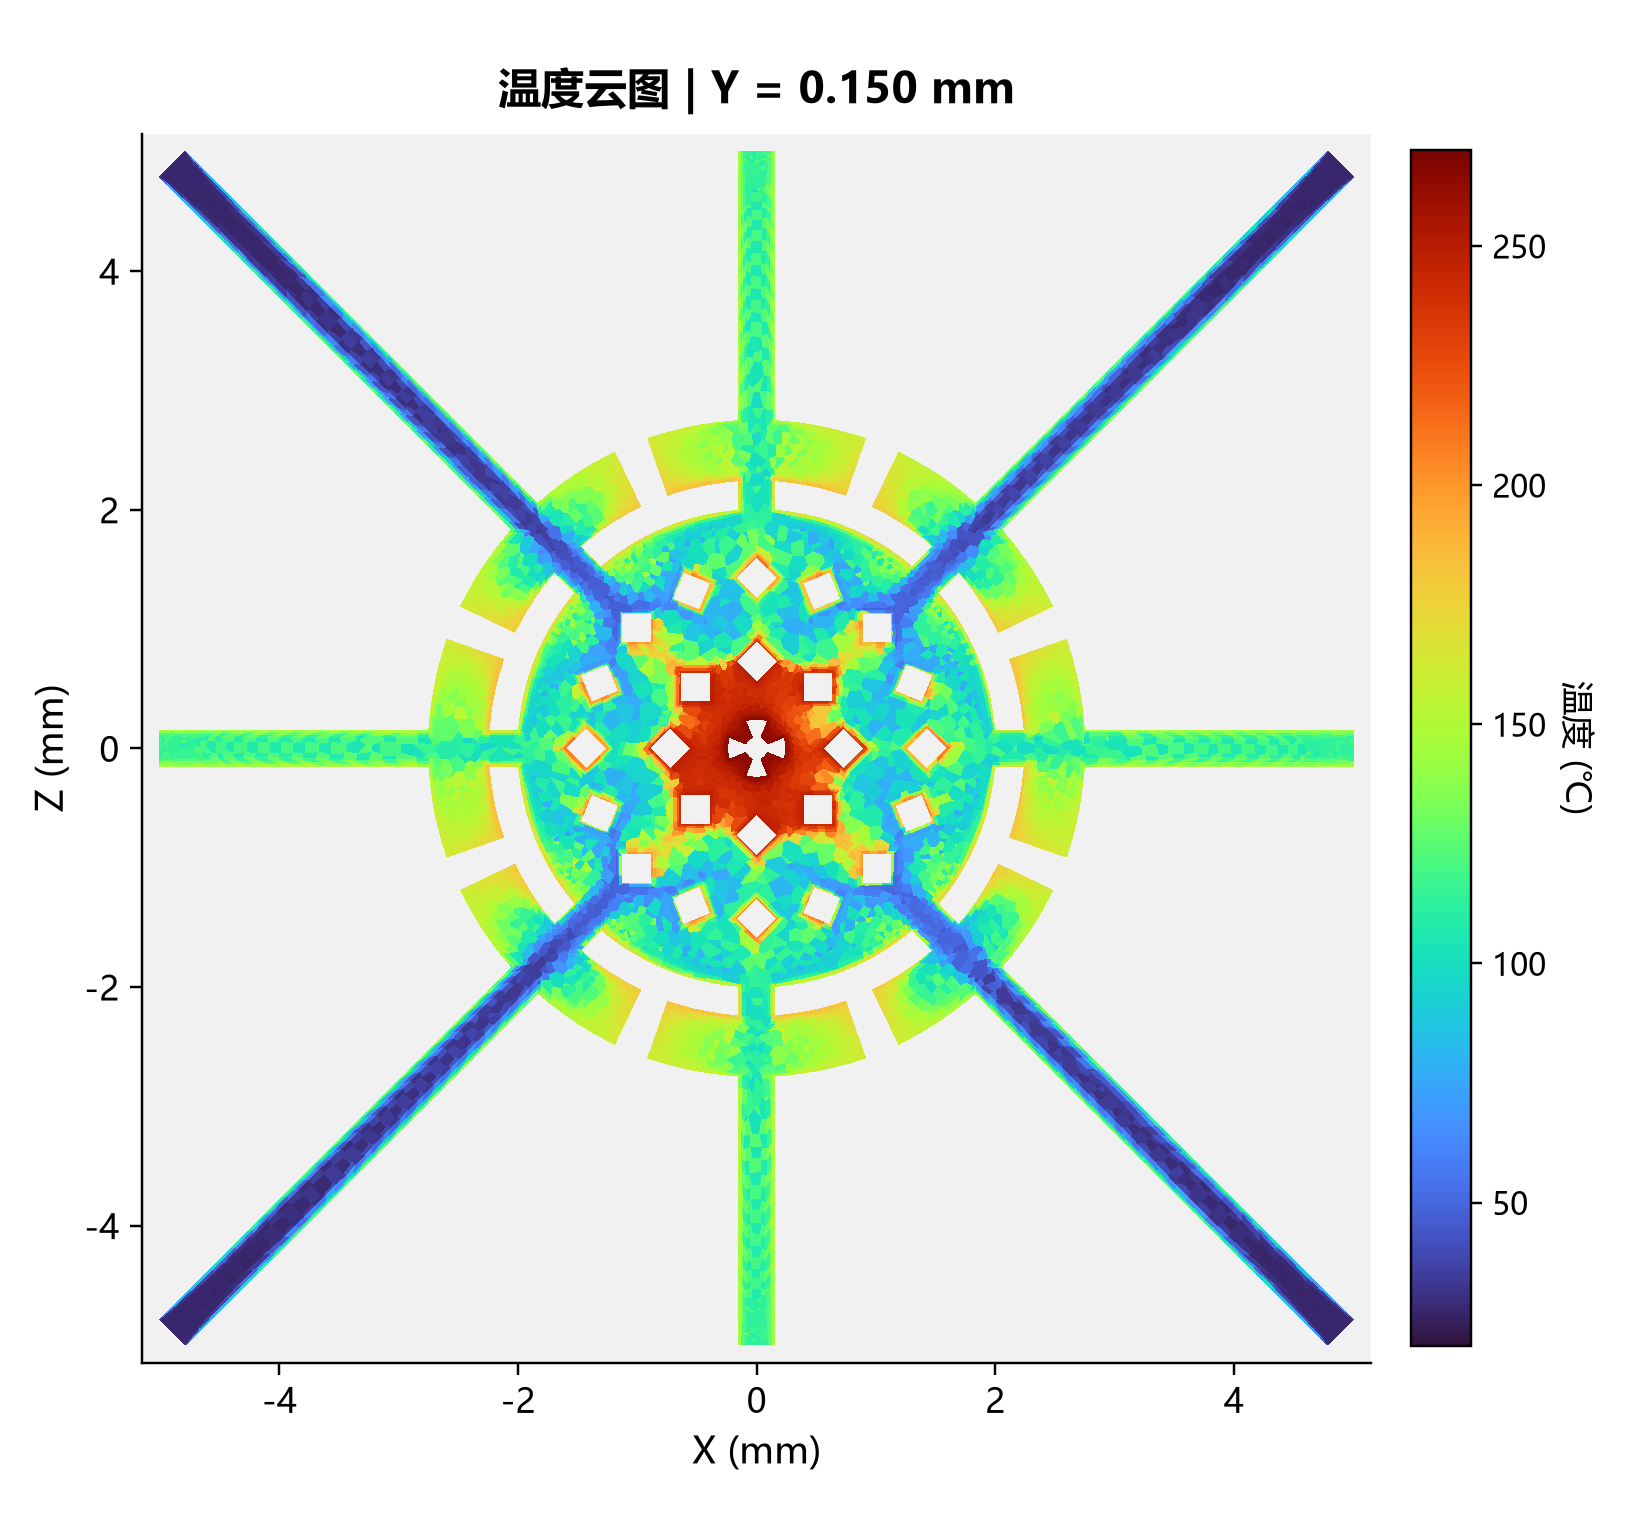
\includegraphics[width=\linewidth]{../../figs/midterm_monthly1_09_temperature_midplane.png}\end{subfigure}\hfill
\begin{subfigure}{.235\linewidth}\centering
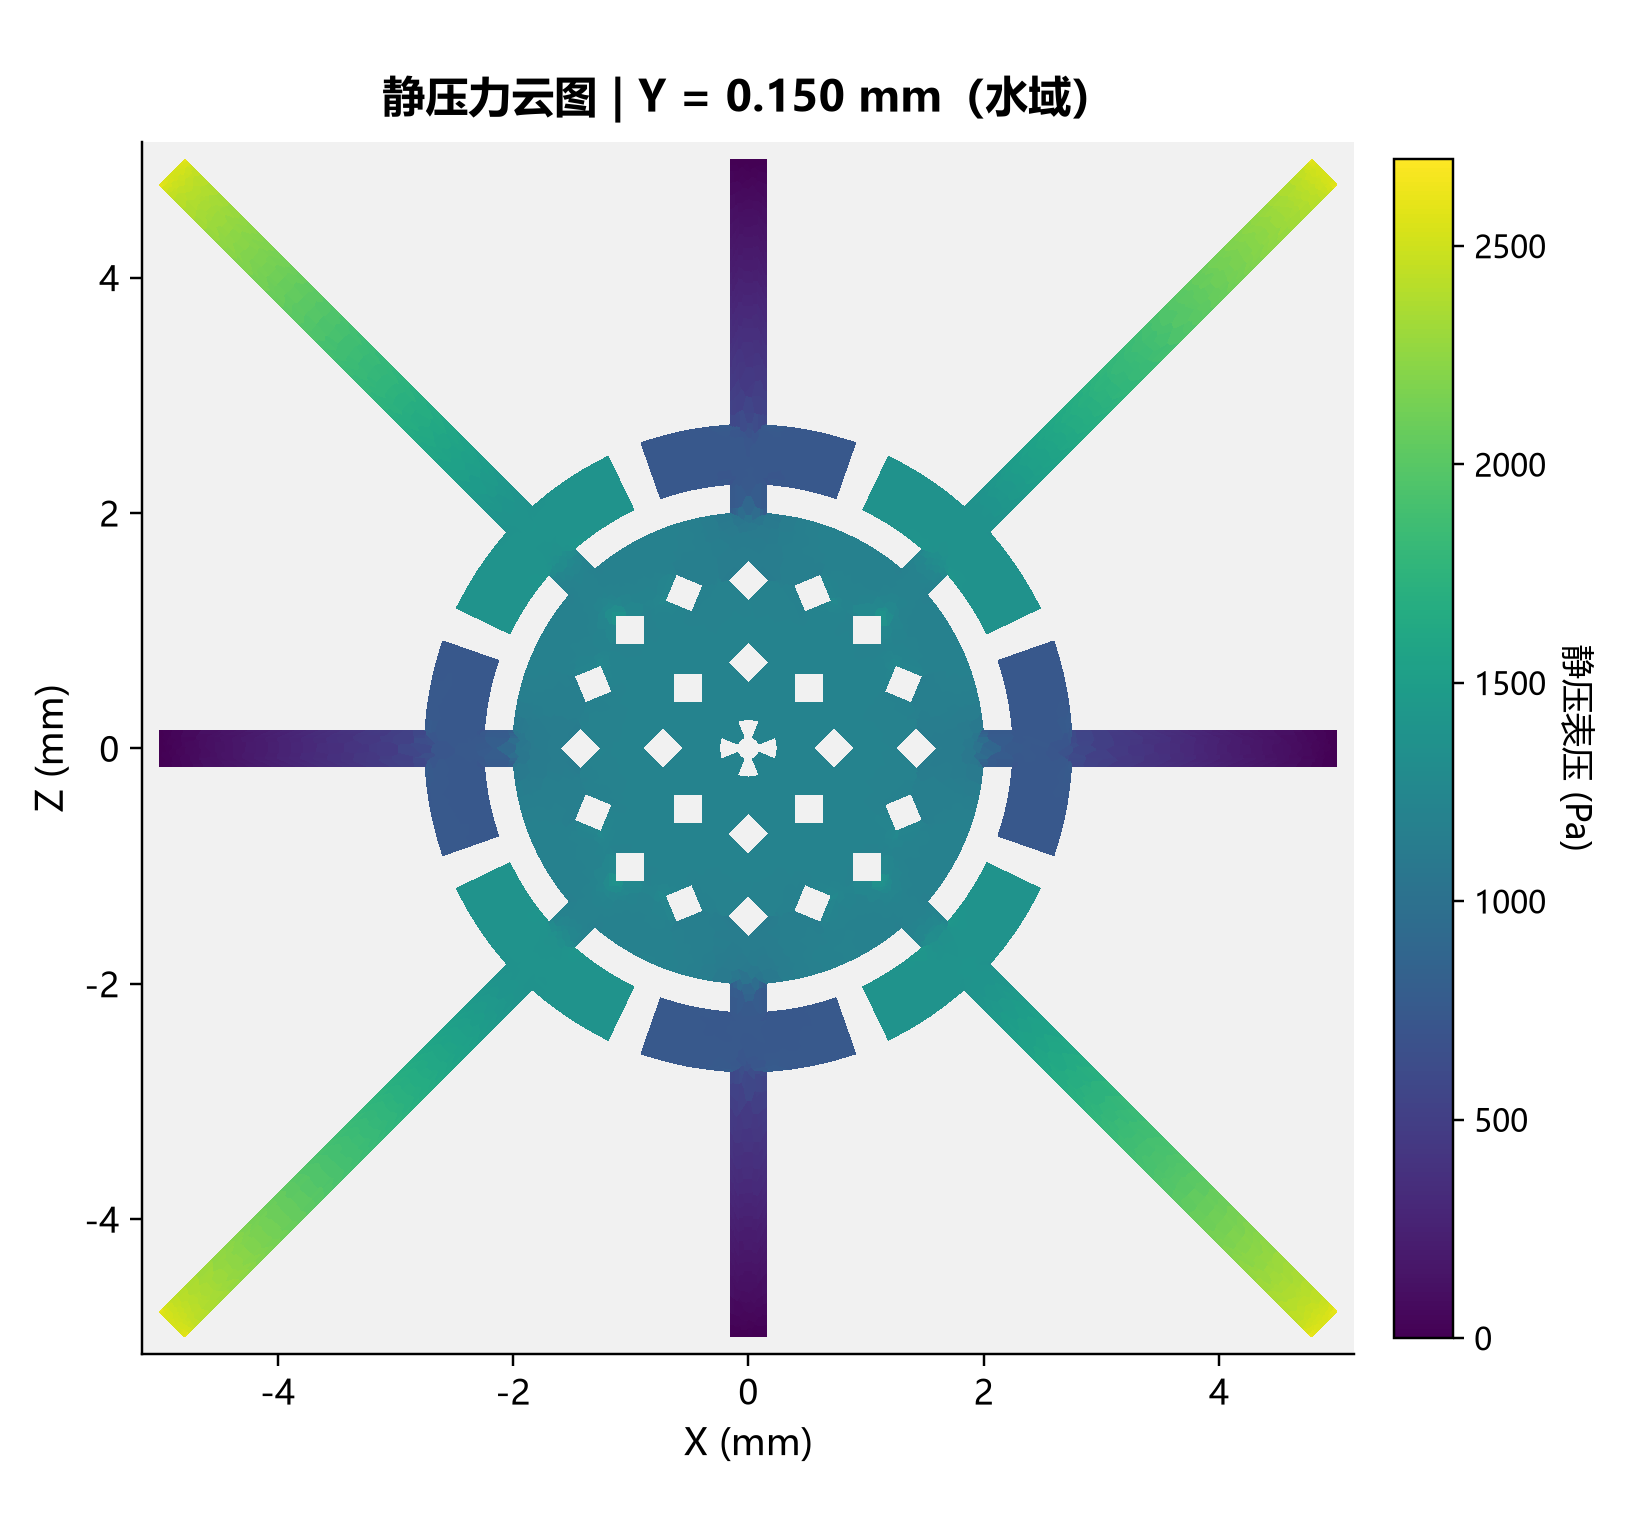
\includegraphics[width=\linewidth]{../../figs/midterm_monthly1_10_pressure_midplane.png}\end{subfigure}\hfill
\begin{subfigure}{.235\linewidth}\centering
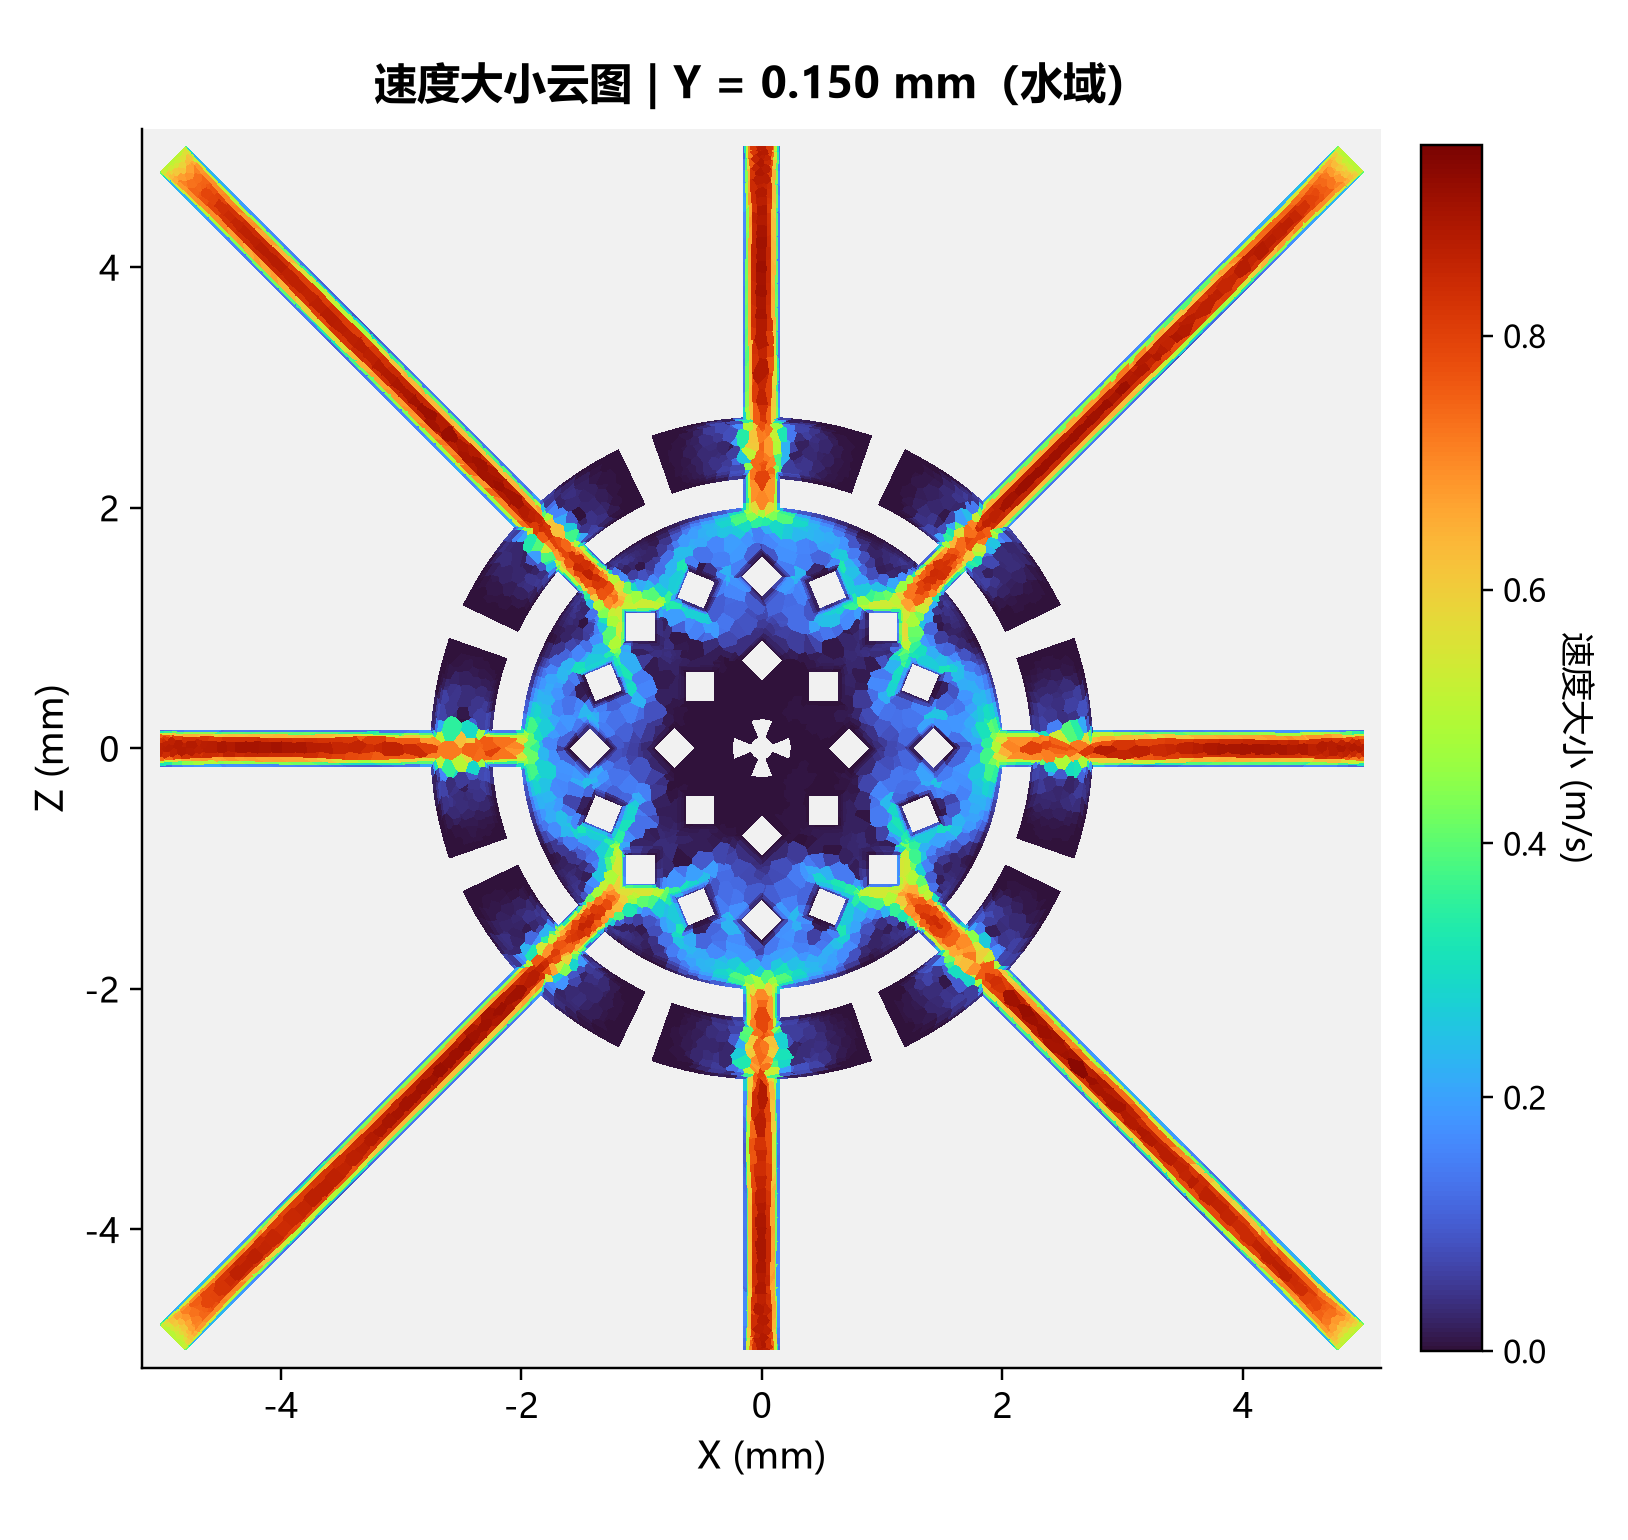
\includegraphics[width=\linewidth]{../../figs/midterm_monthly1_11_speed_midplane.png}\end{subfigure}\hfill
\begin{subfigure}{.235\linewidth}\centering
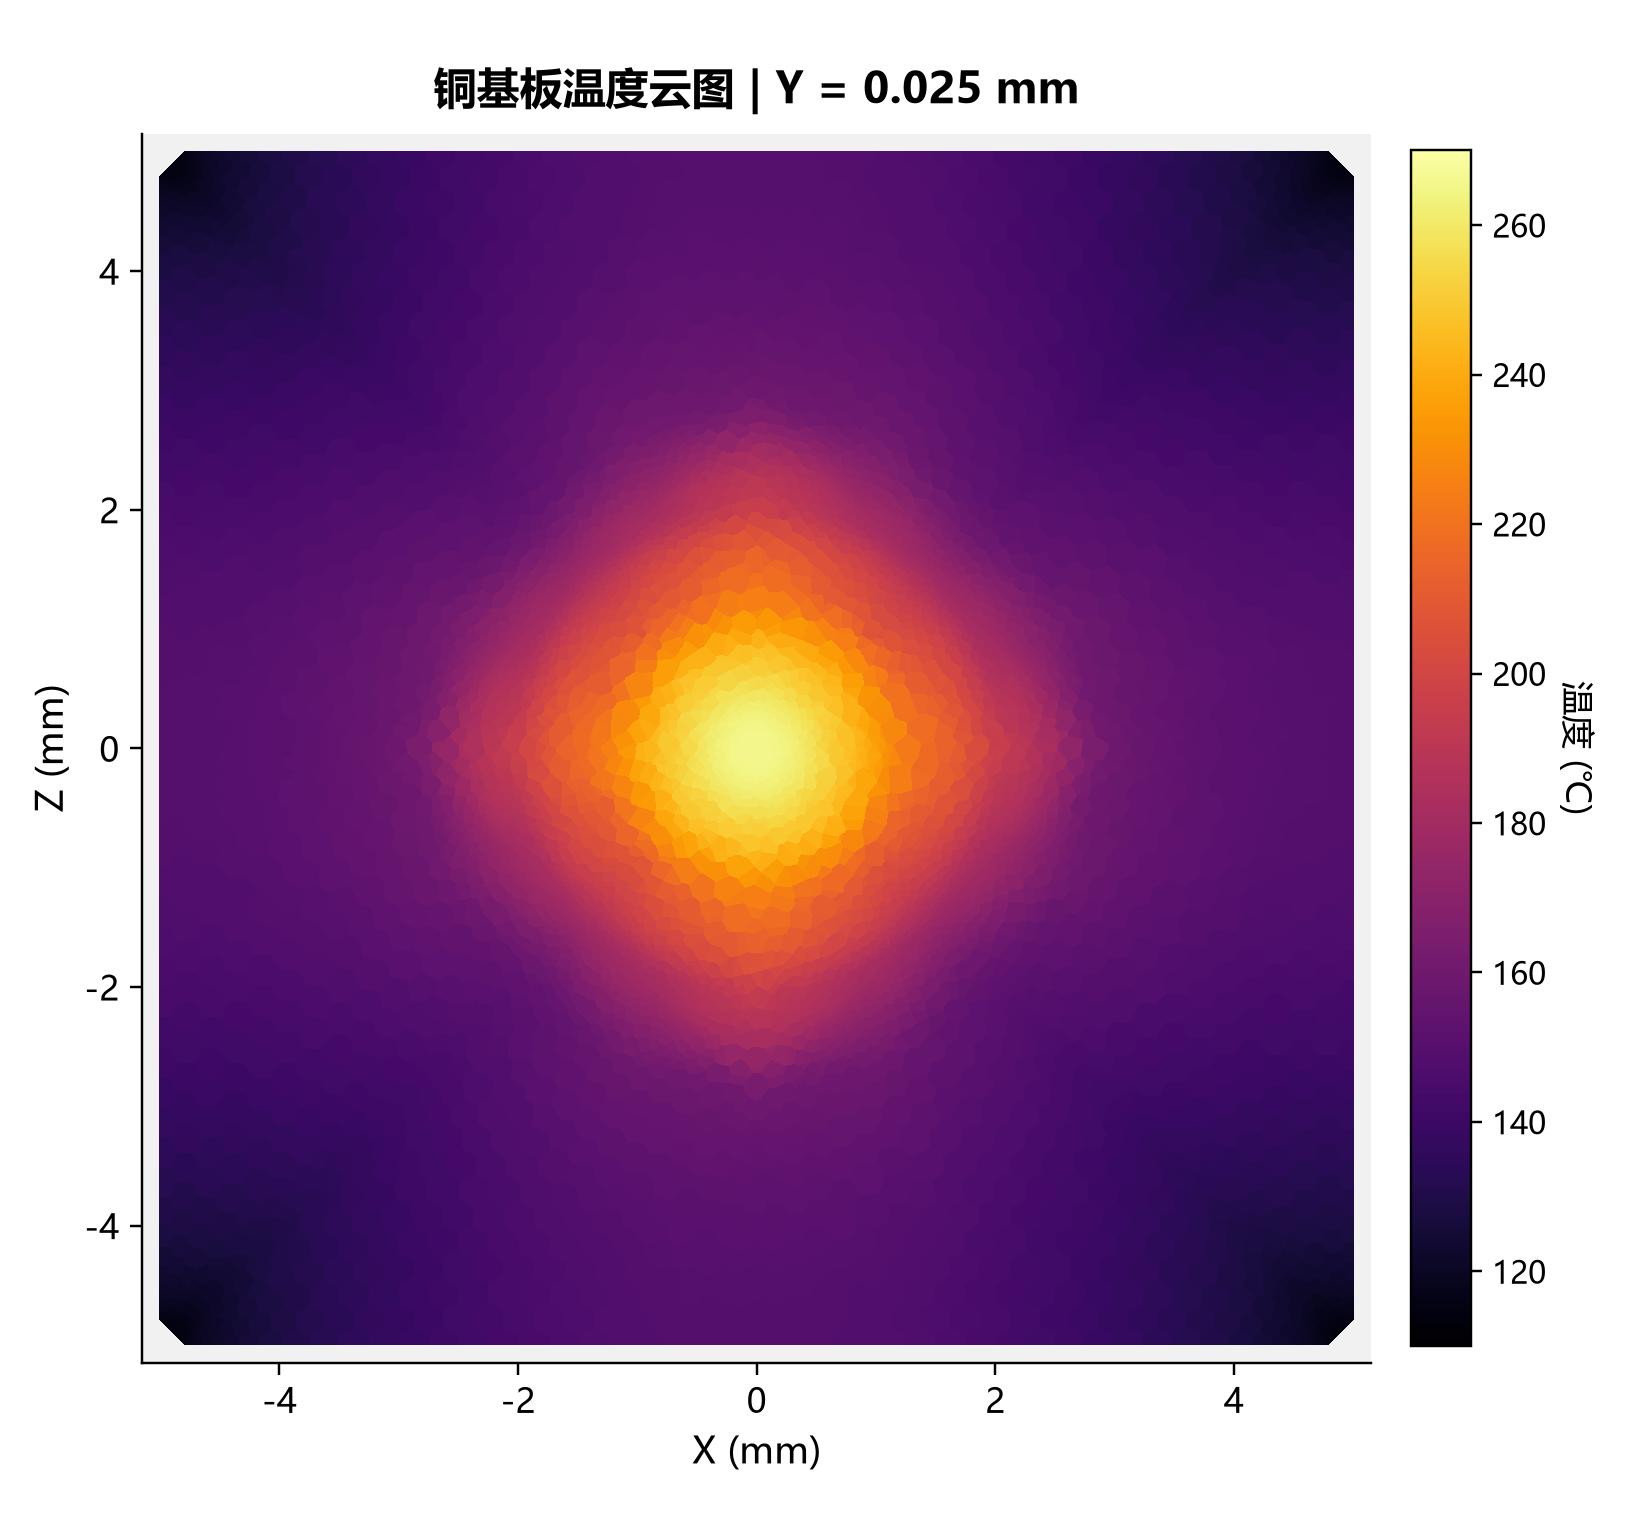
\includegraphics[width=\linewidth]{../../figs/midterm_monthly1_12_copper_base_temperature.png}\end{subfigure}
\caption{三组流道的复现云图：自上而下为方形、六边形与圆形微通道，自左至右为水侧温度、水侧表压、水侧速度大小与铜基板温度。水侧取 $Y=0.150$ mm，铜基板取 $Y=0.025$ mm；保留各图原色标，不能由颜色直接比较不同工况。}
\label{fig:repro}
\end{figure}
\clearpage
\setcounter{section}{3}
\setcounter{table}{1}
\begin{table}[!htbp]
\centering\small
\caption{NACA2416\_v3七档网格在0.2 s的已有结果}\label{tab:04}
\begin{tabularx}{\linewidth}{lYYY}
\toprule
\rowcolor{ydzjlight} 单元数 & 平均温度/K & 最高温度/K & 静压差/Pa \\
\midrule
260169 & 304.668393 & 344.675487 & 2505.203605 \\
575129 & 304.411275 & 345.265735 & 2389.274100 \\
1073583 & 303.944909 & 345.153612 & 2440.765641 \\
1524876 & 305.093298 & 346.048803 & 2389.938449 \\
2943269 & 304.373551 & 345.964030 & 2355.838476 \\
3235081 & 304.300924 & 345.983833 & 2348.320348 \\
4610769 & 305.985989 & 346.618797 & 2448.714104 \\
\bottomrule
\end{tabularx}
\par\smallskip\begin{minipage}{\linewidth}\footnotesize 温度为全域单元算术平均及全域最高值，静压为进出口面积平均；非受热面指标。最细档有不同时间步历史，未通过全序列1\%联合判据。来源：配套源码目录内 evidence/mesh\_results\_02s.csv。—。\end{minipage}
\end{table}
\clearpage
\setcounter{section}{3}
\setcounter{figure}{1}
\begin{figure}[!htbp]\centering
\begin{subfigure}{0.49\linewidth}\centering
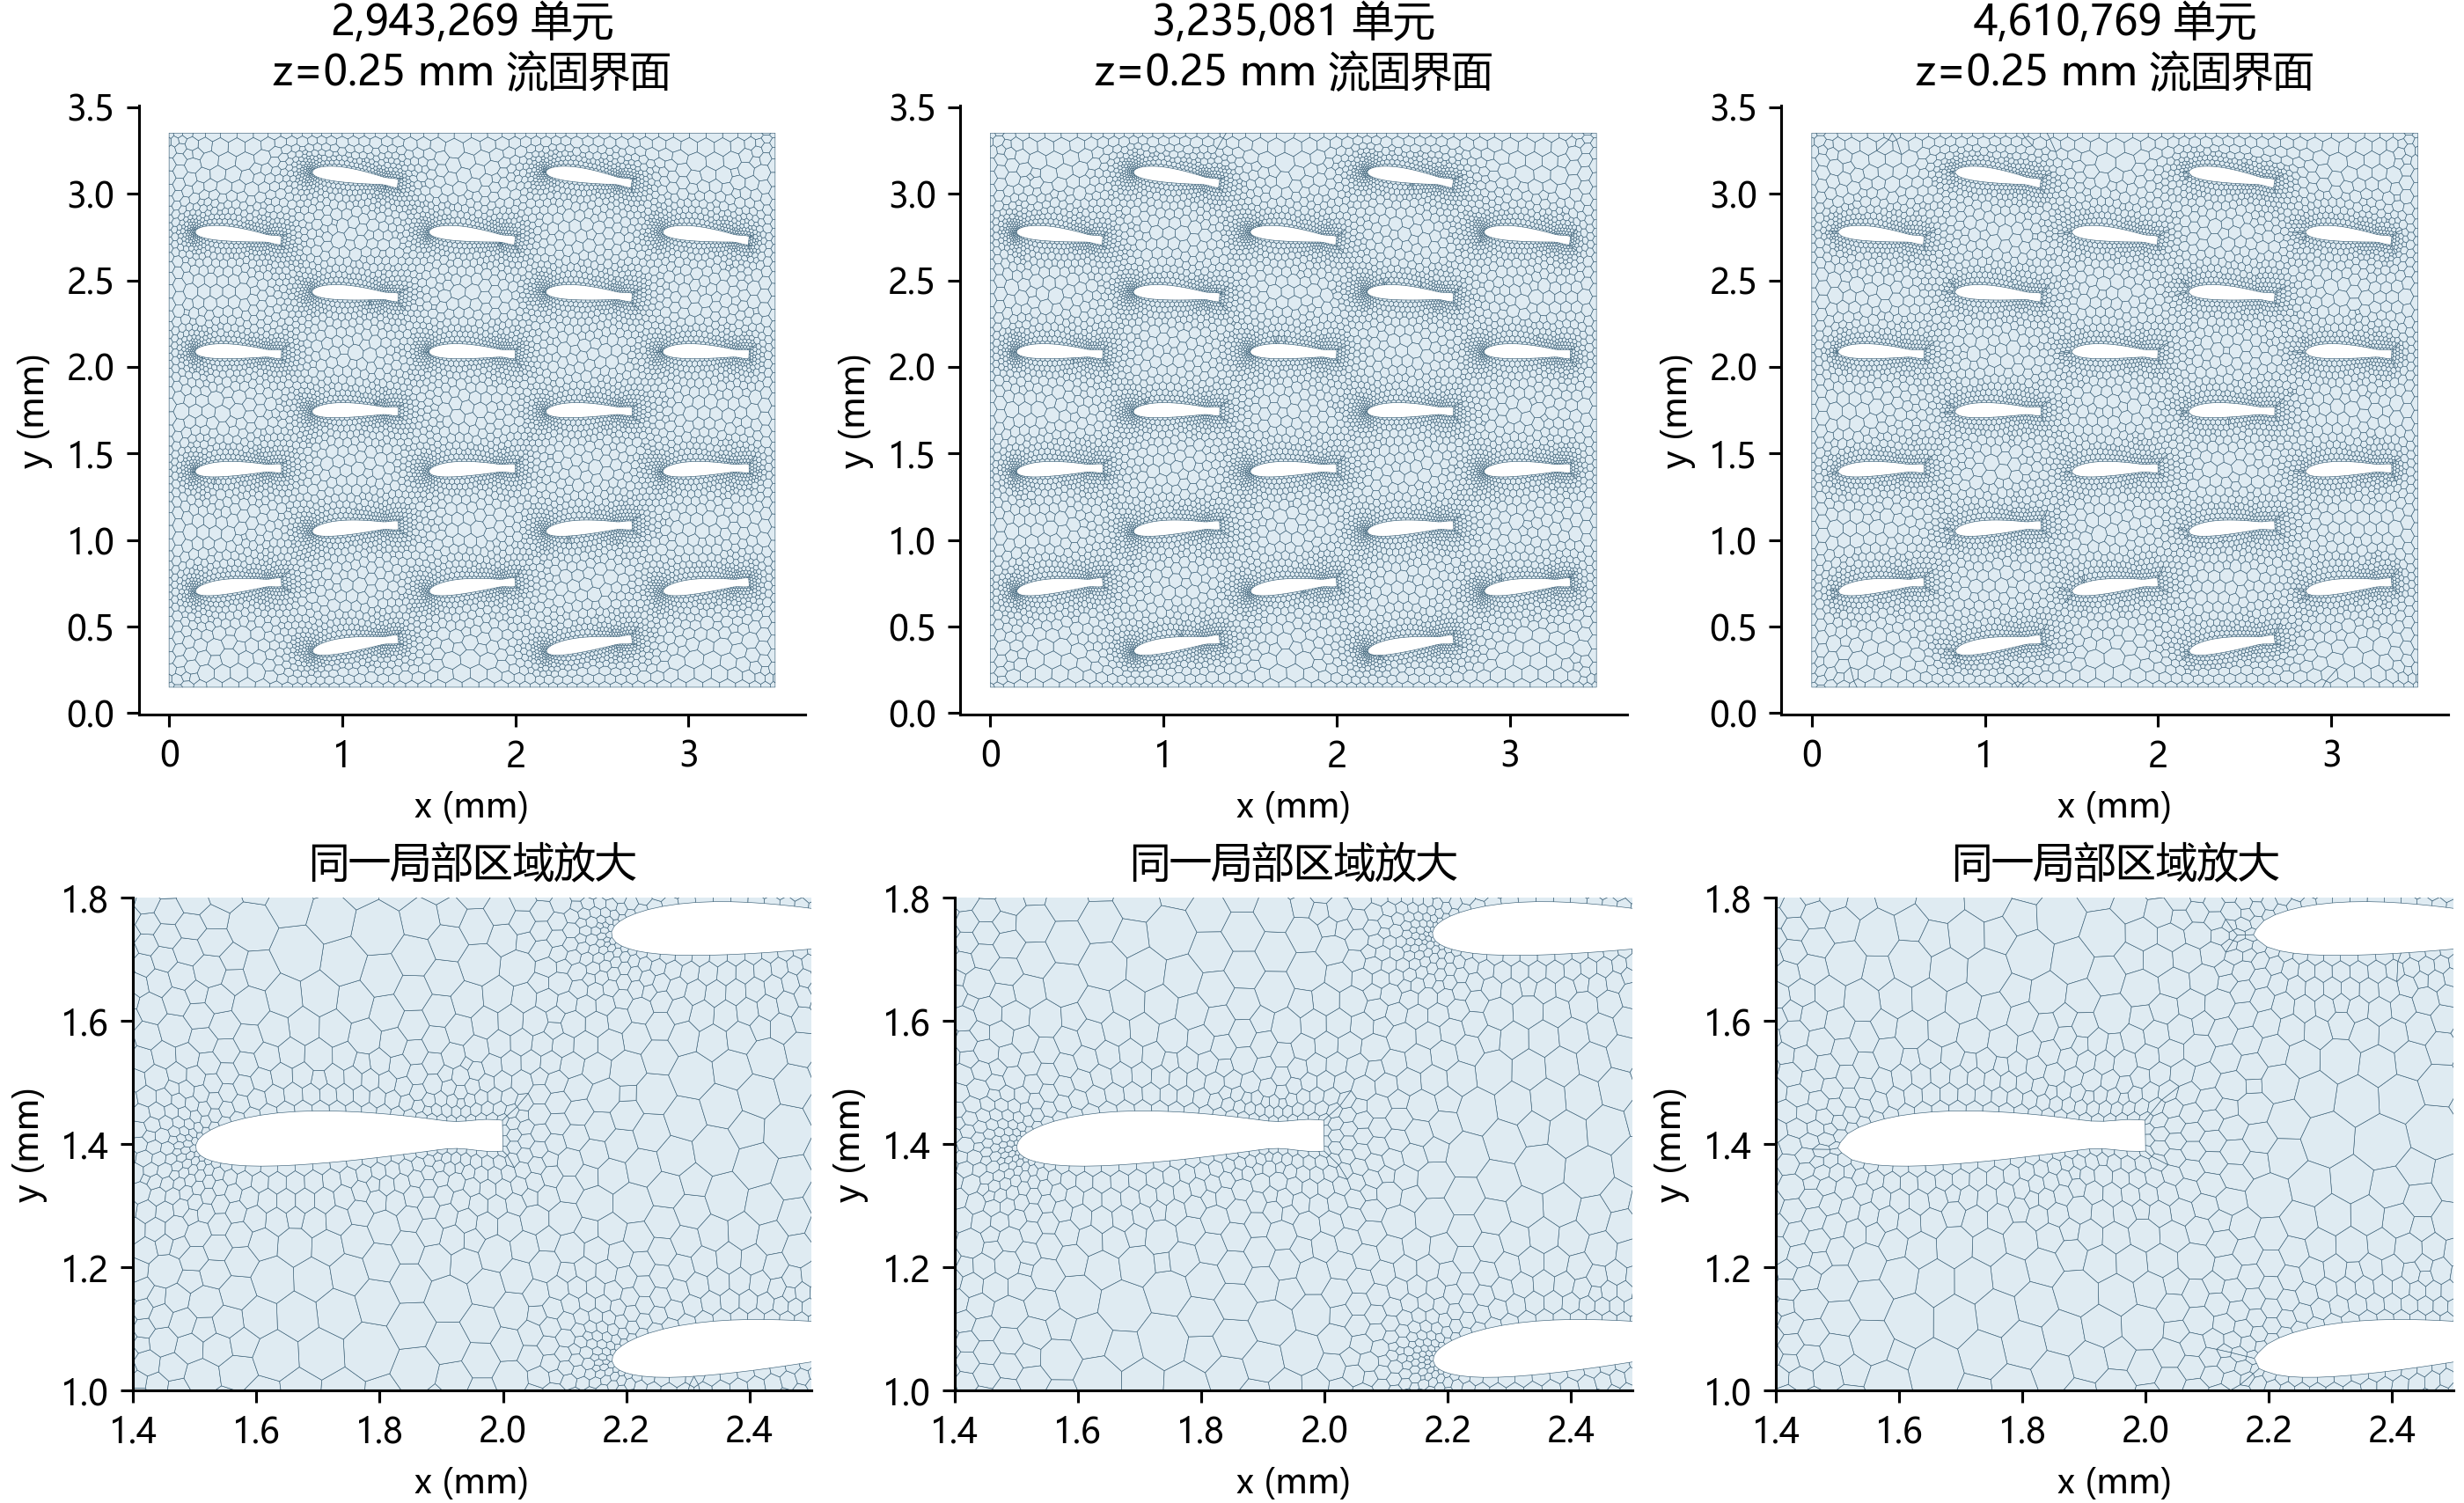
\includegraphics[width=\linewidth]{../../figs/midterm_asset_naca_mesh_actual.png}
\caption{NACA2416 v3三档实际流固界面面网格，统一取 z=0.25 mm。下排采用相同局部范围；此图不等同于三维边界层截面，单元总数增大也不保证每一局部区域同步加密。}\label{fig:08}
\end{subfigure}\hfill
\begin{subfigure}{0.49\linewidth}\centering
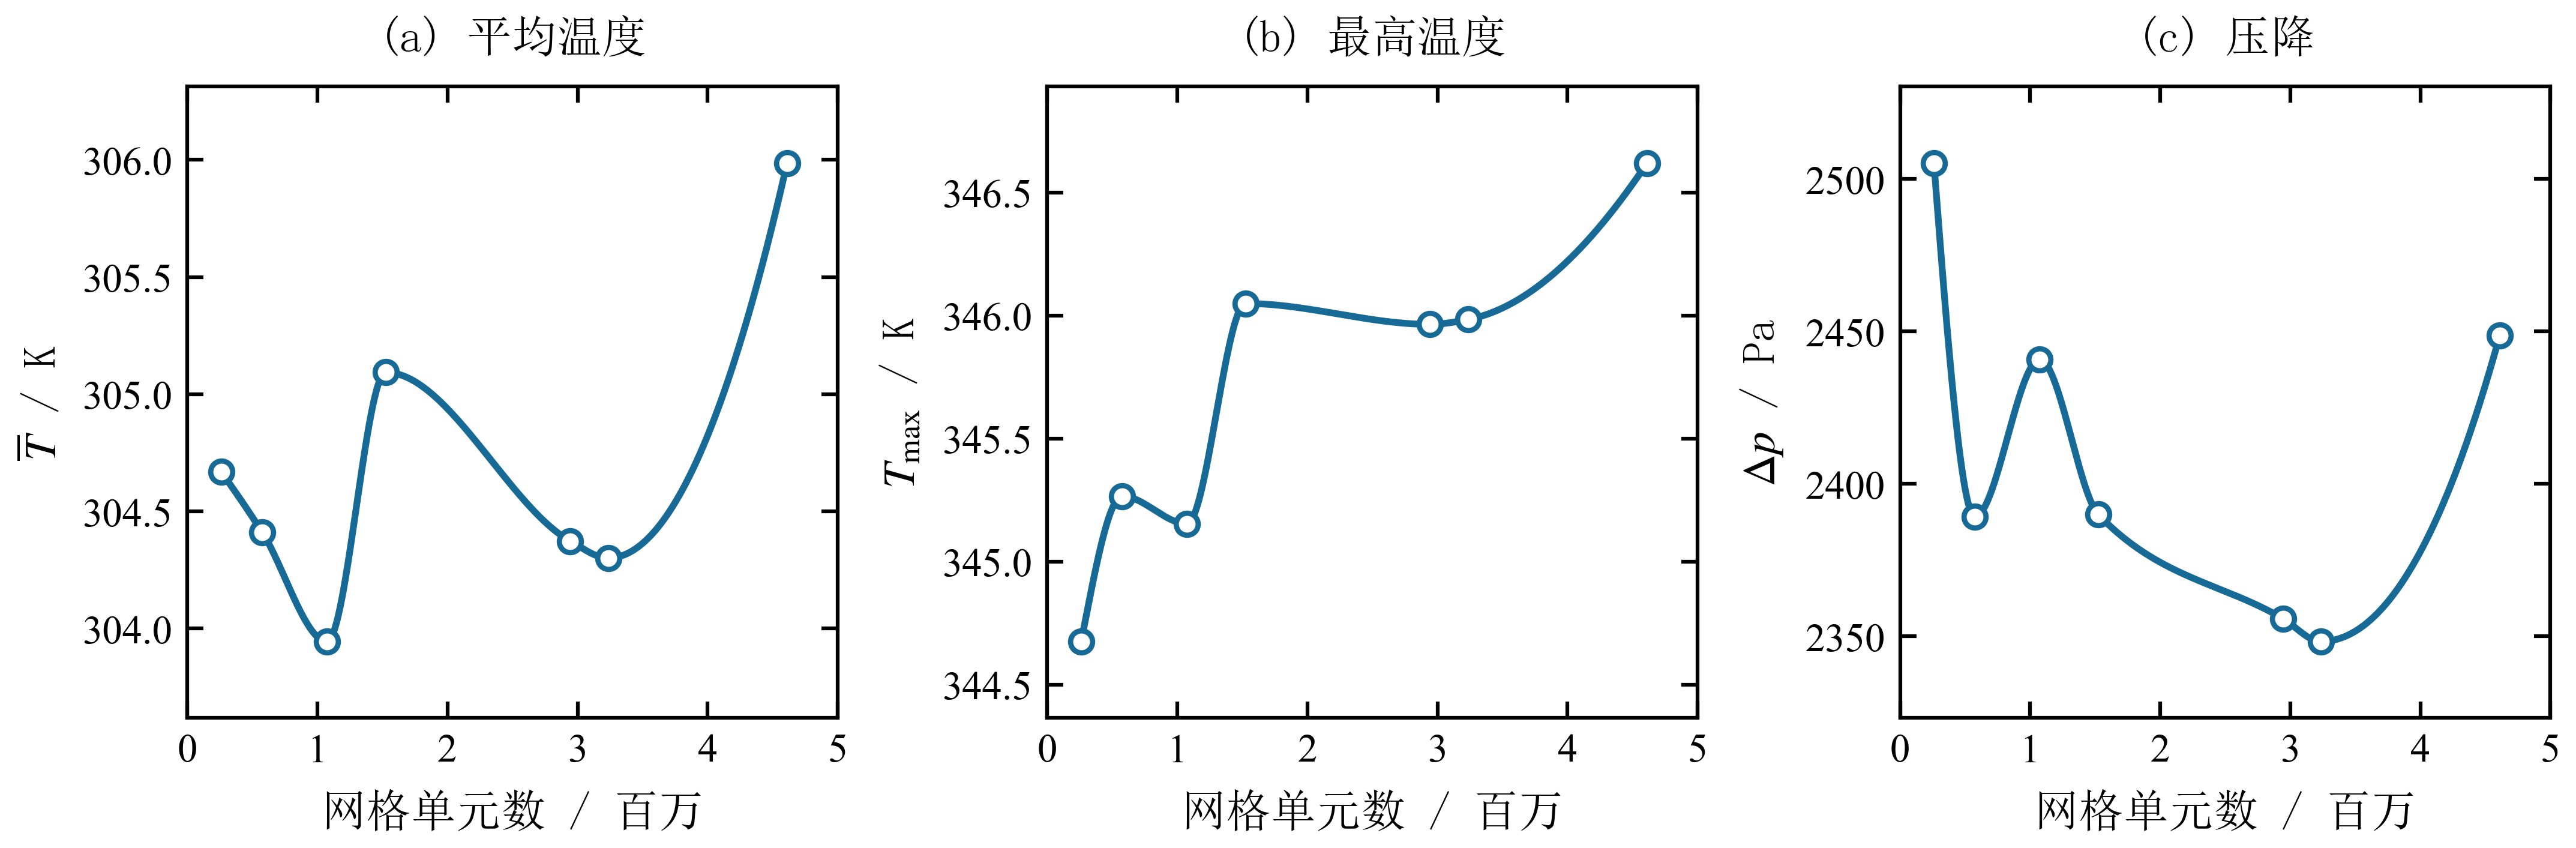
\includegraphics[width=\linewidth]{../../figs/midterm_month3_mesh_temperature_pressure.png}
\caption{NACA2416在0.2 s的七档网格温度与静压差，沿用原始保存数据。}\label{fig:09}
\end{subfigure}
\caption{流固界面面网格与七档网格温度、静压差}
\end{figure}
\clearpage
\setcounter{section}{3}
\setcounter{table}{2}
\begin{table}[!htbp]\centering
\caption{以323万档为参考的温度与压降相对差异（\%）}
\label{m3:tab:mesh_ref323}
\begin{tabular*}{\textwidth}{@{\extracolsep{\fill}}rrrr@{}}\toprule
\rowcolor{ydzjlight} 单元数 / 万 & 平均温度差异 & 最高温度差异 & 压降差异 \\
\midrule
26.02 & 0.1208 & 0.3782 & 6.6807 \\
57.51 & 0.0363 & 0.2076 & 1.7440 \\
107.36 & 0.1170 & 0.2400 & 3.9367 \\
152.49 & 0.2604 & 0.0188 & 1.7722 \\
294.33 & 0.0239 & 0.0057 & 0.3201 \\
323.51 & 0.0000 & 0.0000 & 0.0000 \\
461.08 & 0.5537 & 0.1835 & 4.2751 \\
\bottomrule\end{tabular*}\end{table}
\clearpage
\setcounter{section}{3}
\setcounter{figure}{2}
\begin{figure}[!htbp]\centering
\begin{subfigure}{0.49\linewidth}\centering
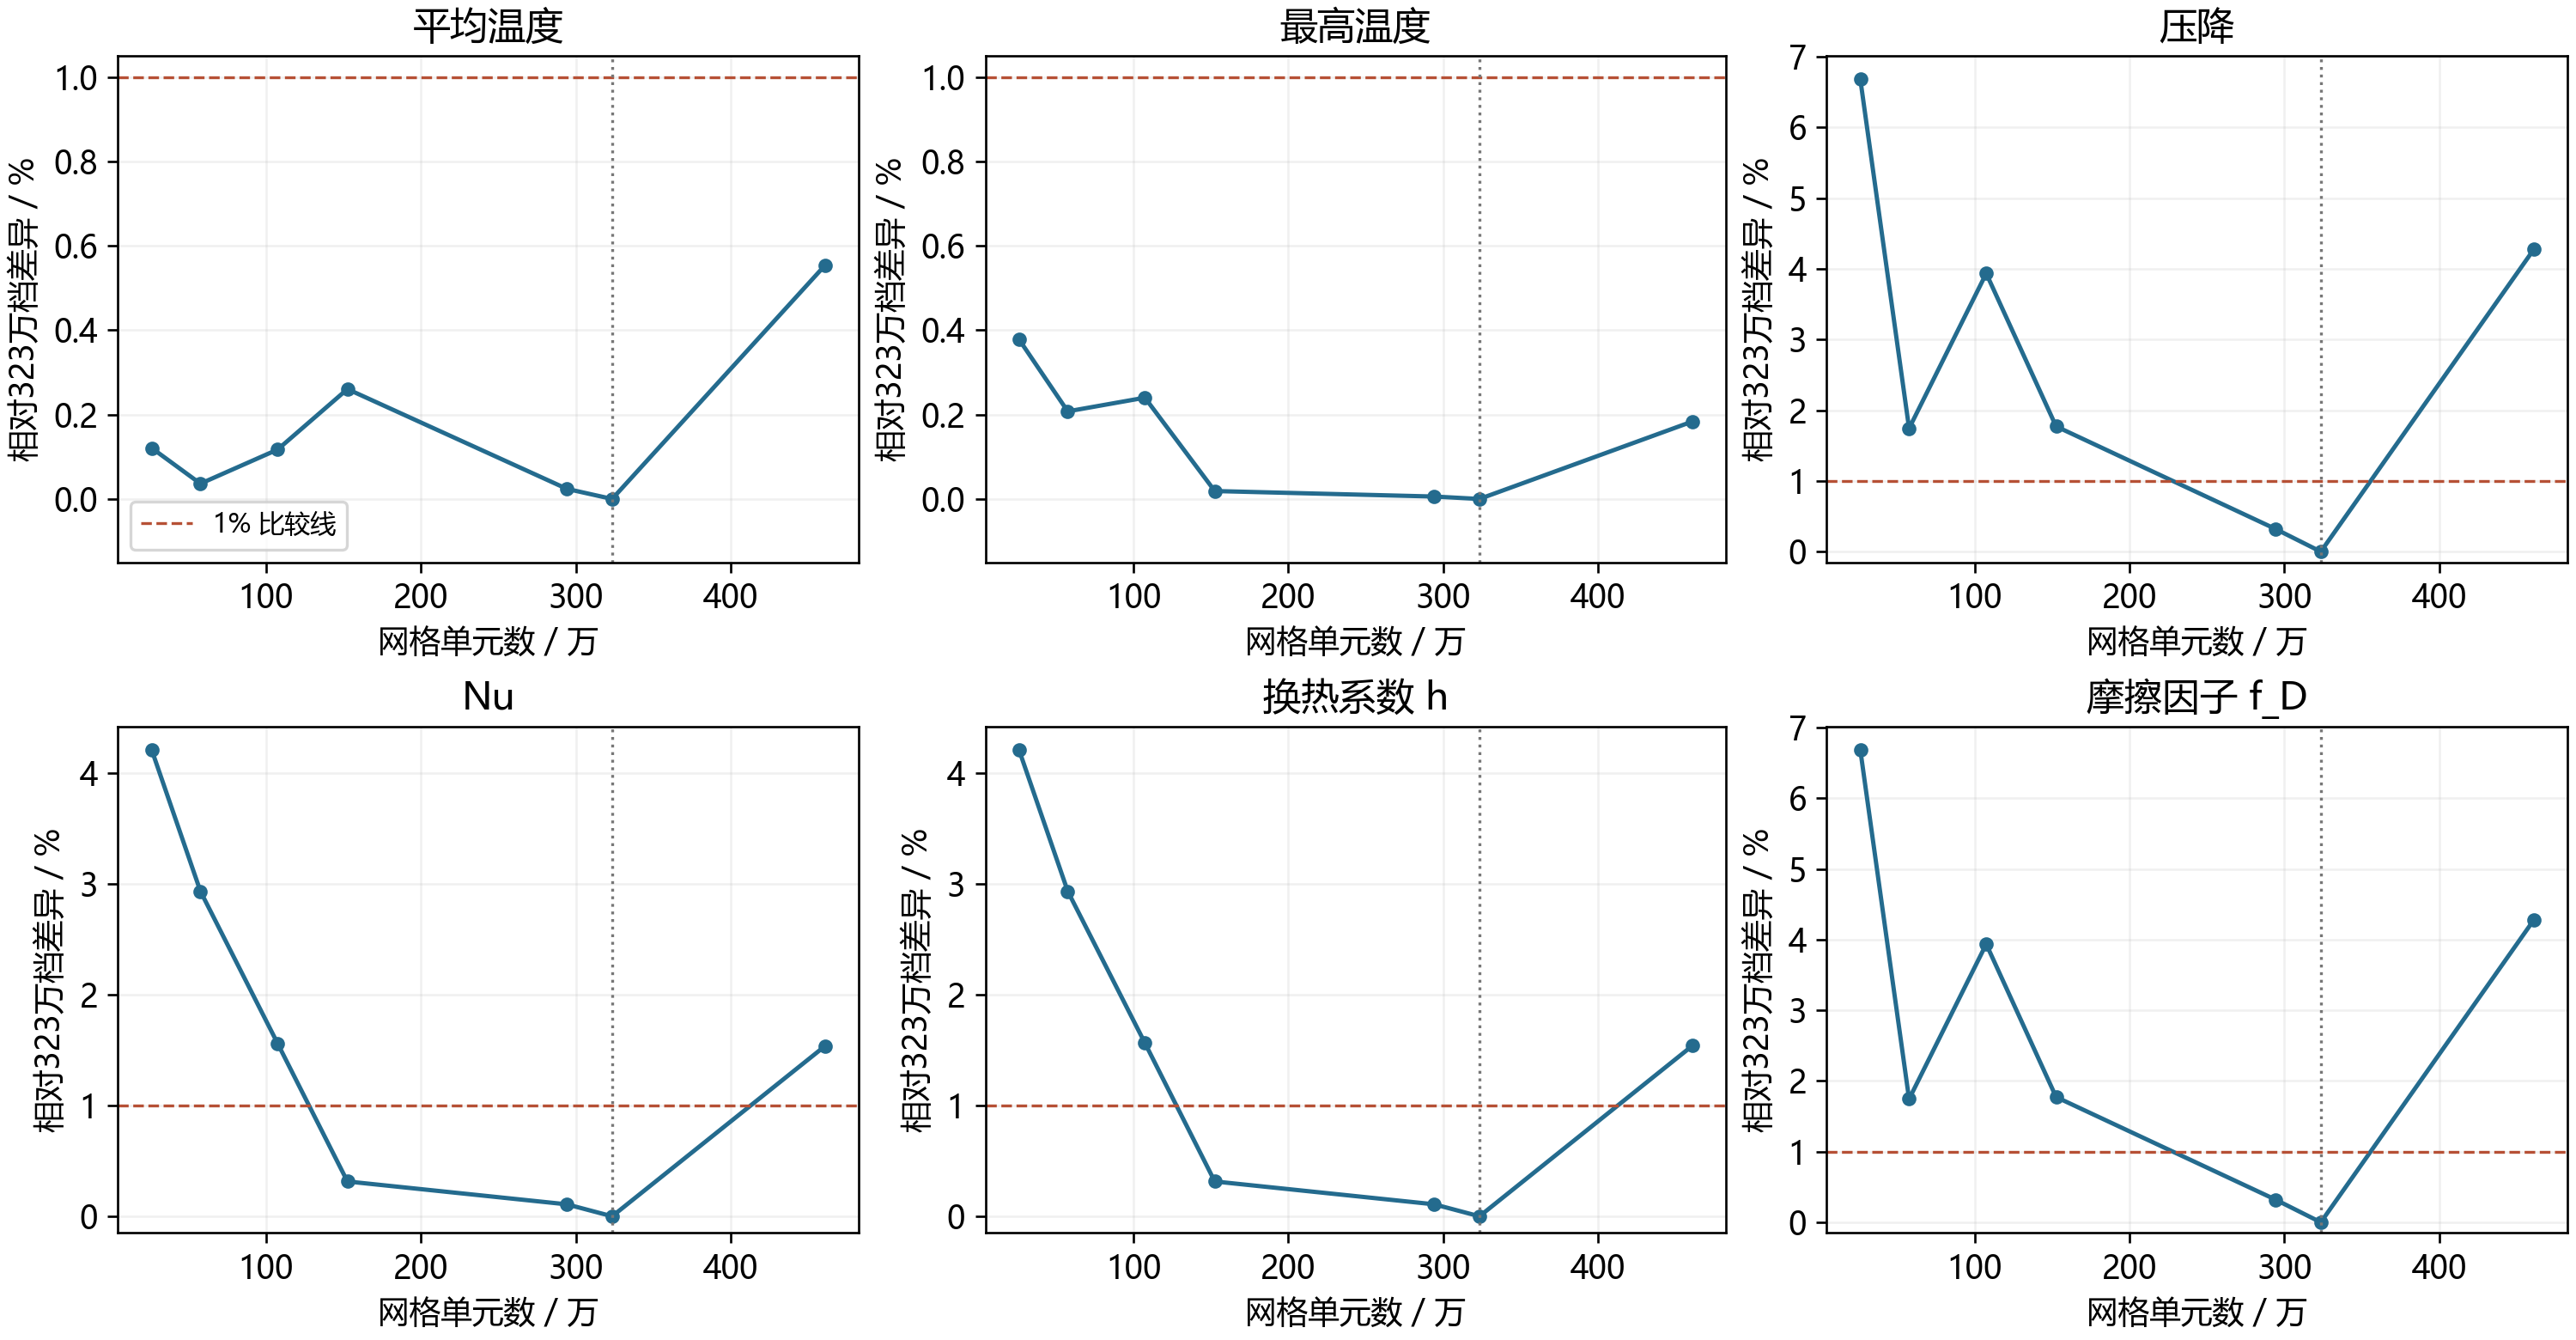
\includegraphics[width=\linewidth]{../../figs/midterm_month3_mesh_errors_ref323.png}
\caption{温度、压降及换热流阻指标统一以323万档为参考的相对差异，虚线为1\%比较线。}\label{fig:mesh-errors}
\end{subfigure}\hfill
\begin{subfigure}{0.49\linewidth}\centering
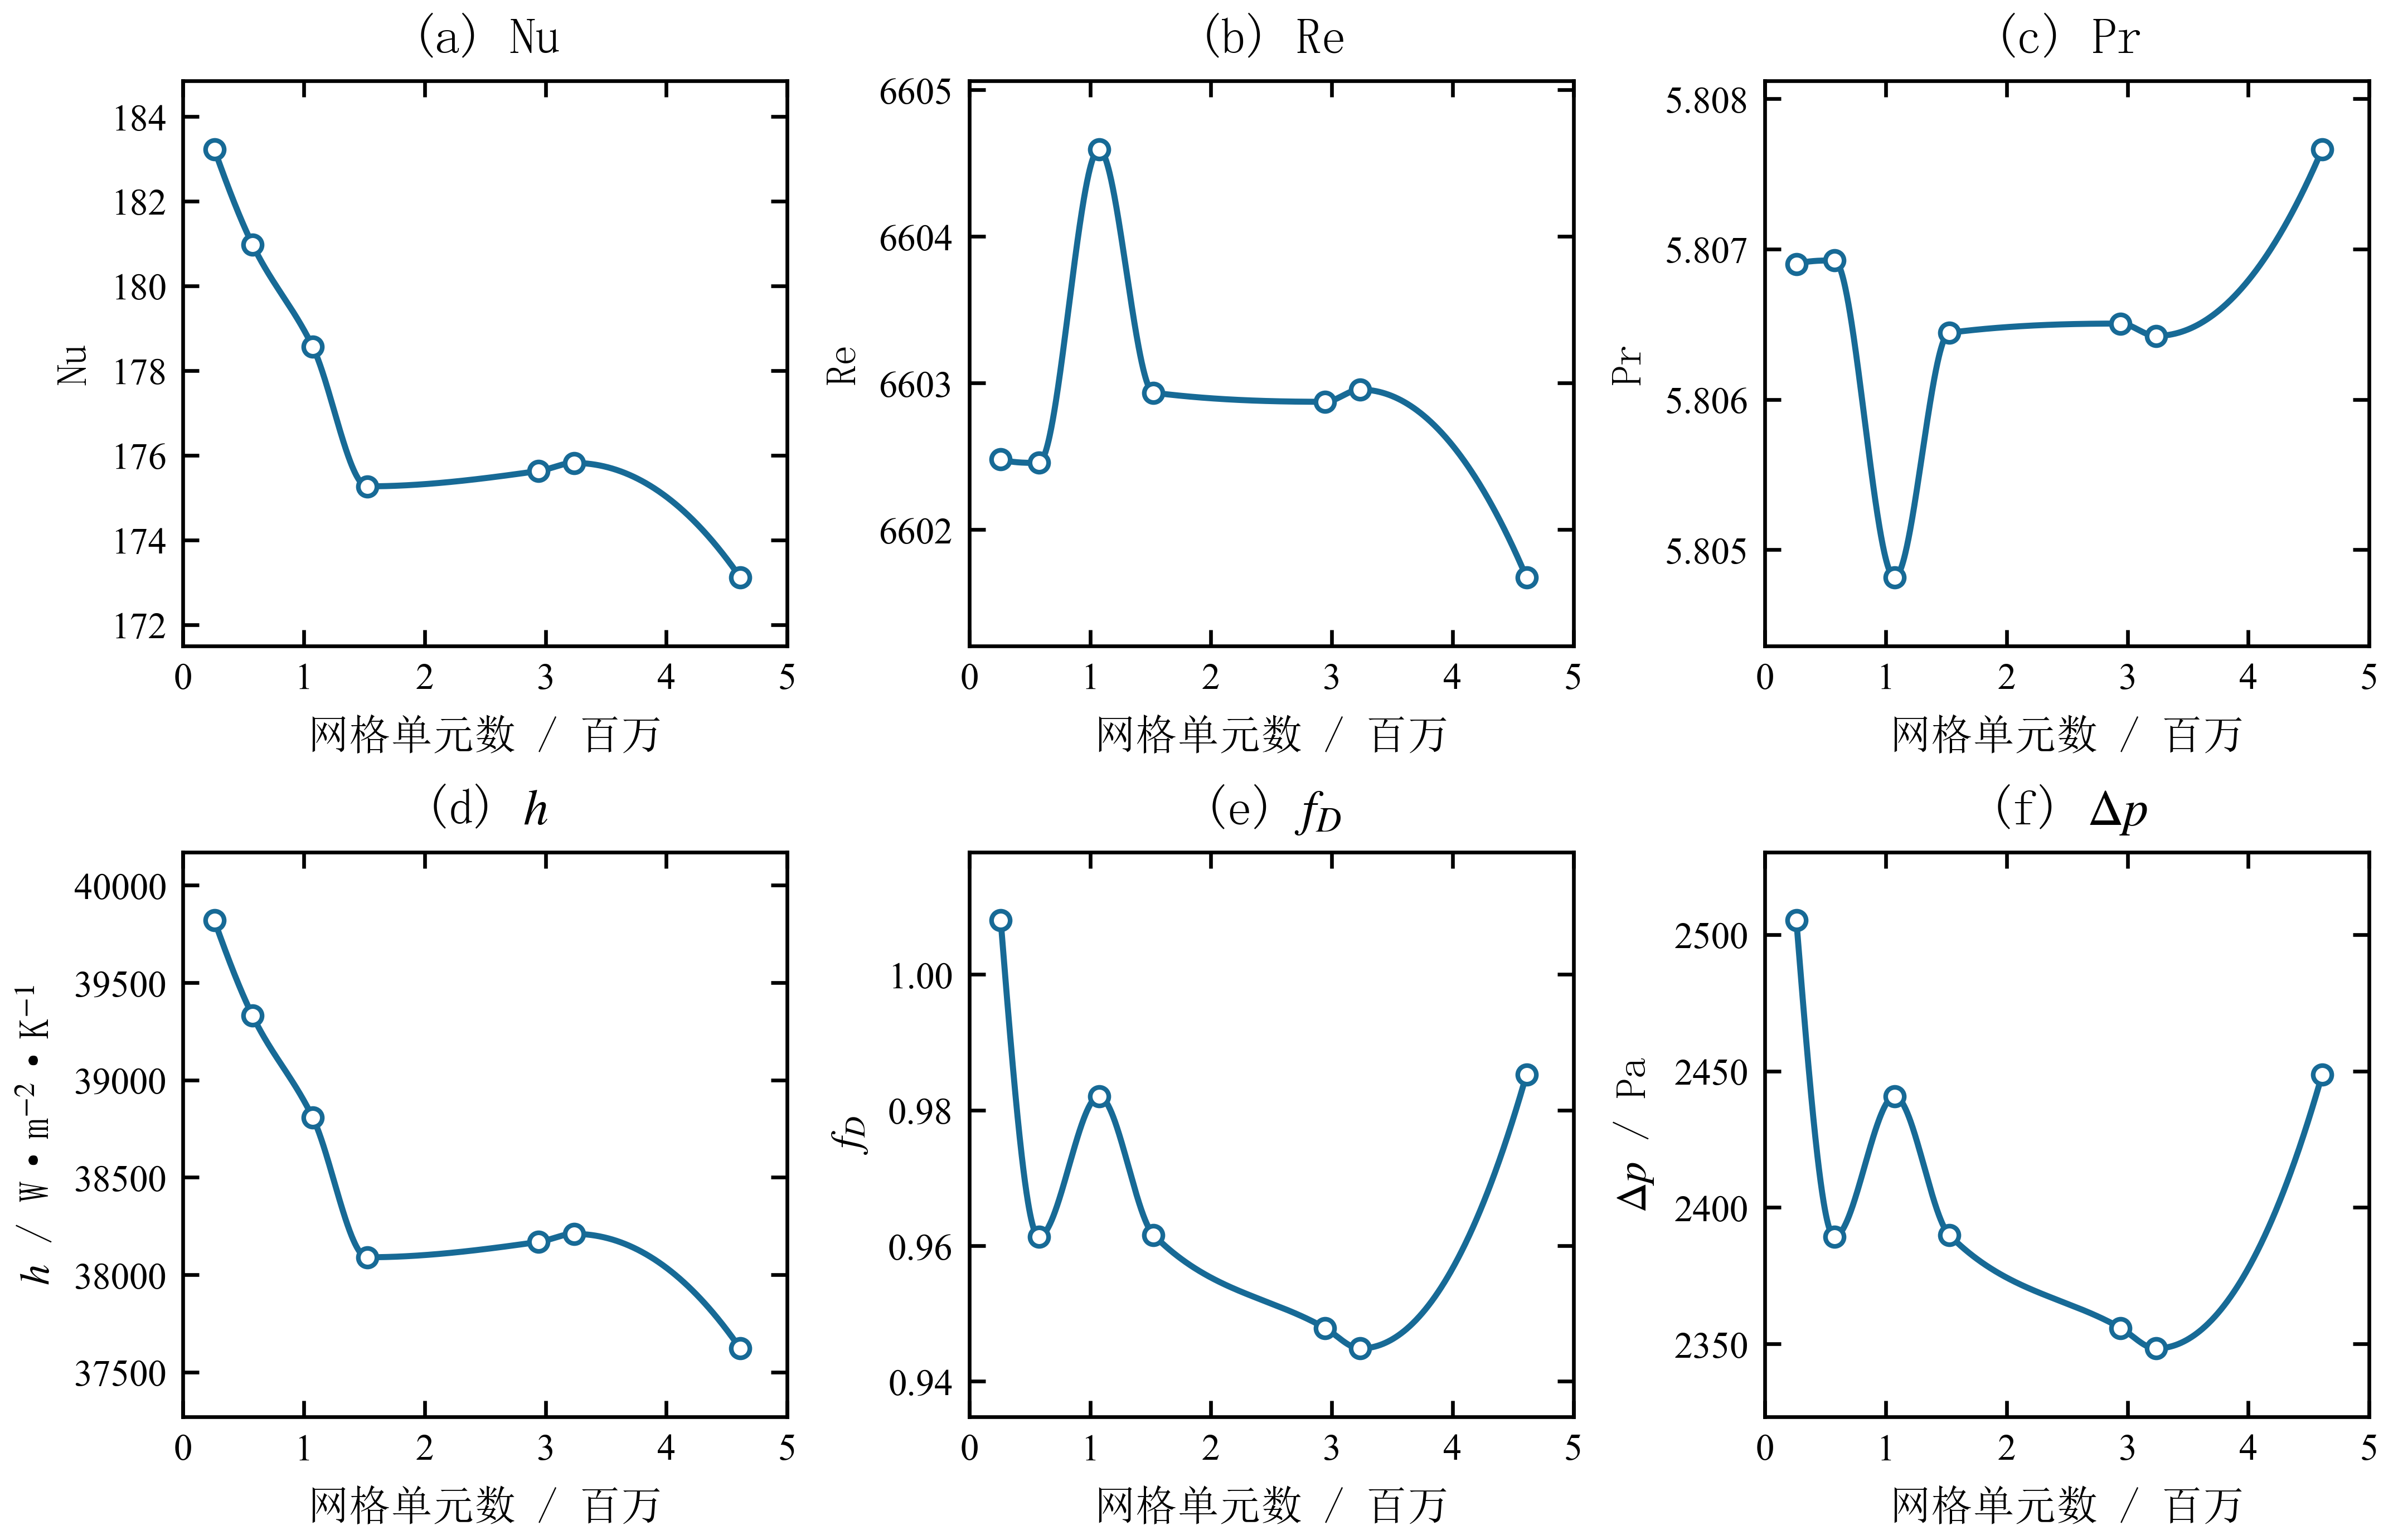
\includegraphics[width=\linewidth]{../../figs/midterm_month3_mesh_dimensionless.png}
\caption{七档网格的换热与流阻指标；特征尺度、物性参考温度及热流统计沿用原始保存记录。}\label{fig:mesh-dimensionless}
\end{subfigure}
\caption{以323万档为参考的相对差异与无量纲换热流阻指标}
\end{figure}
\clearpage
\setcounter{section}{3}
\setcounter{figure}{3}
\begin{figure}[!htbp]\centering
\begin{subfigure}{0.49\linewidth}\centering
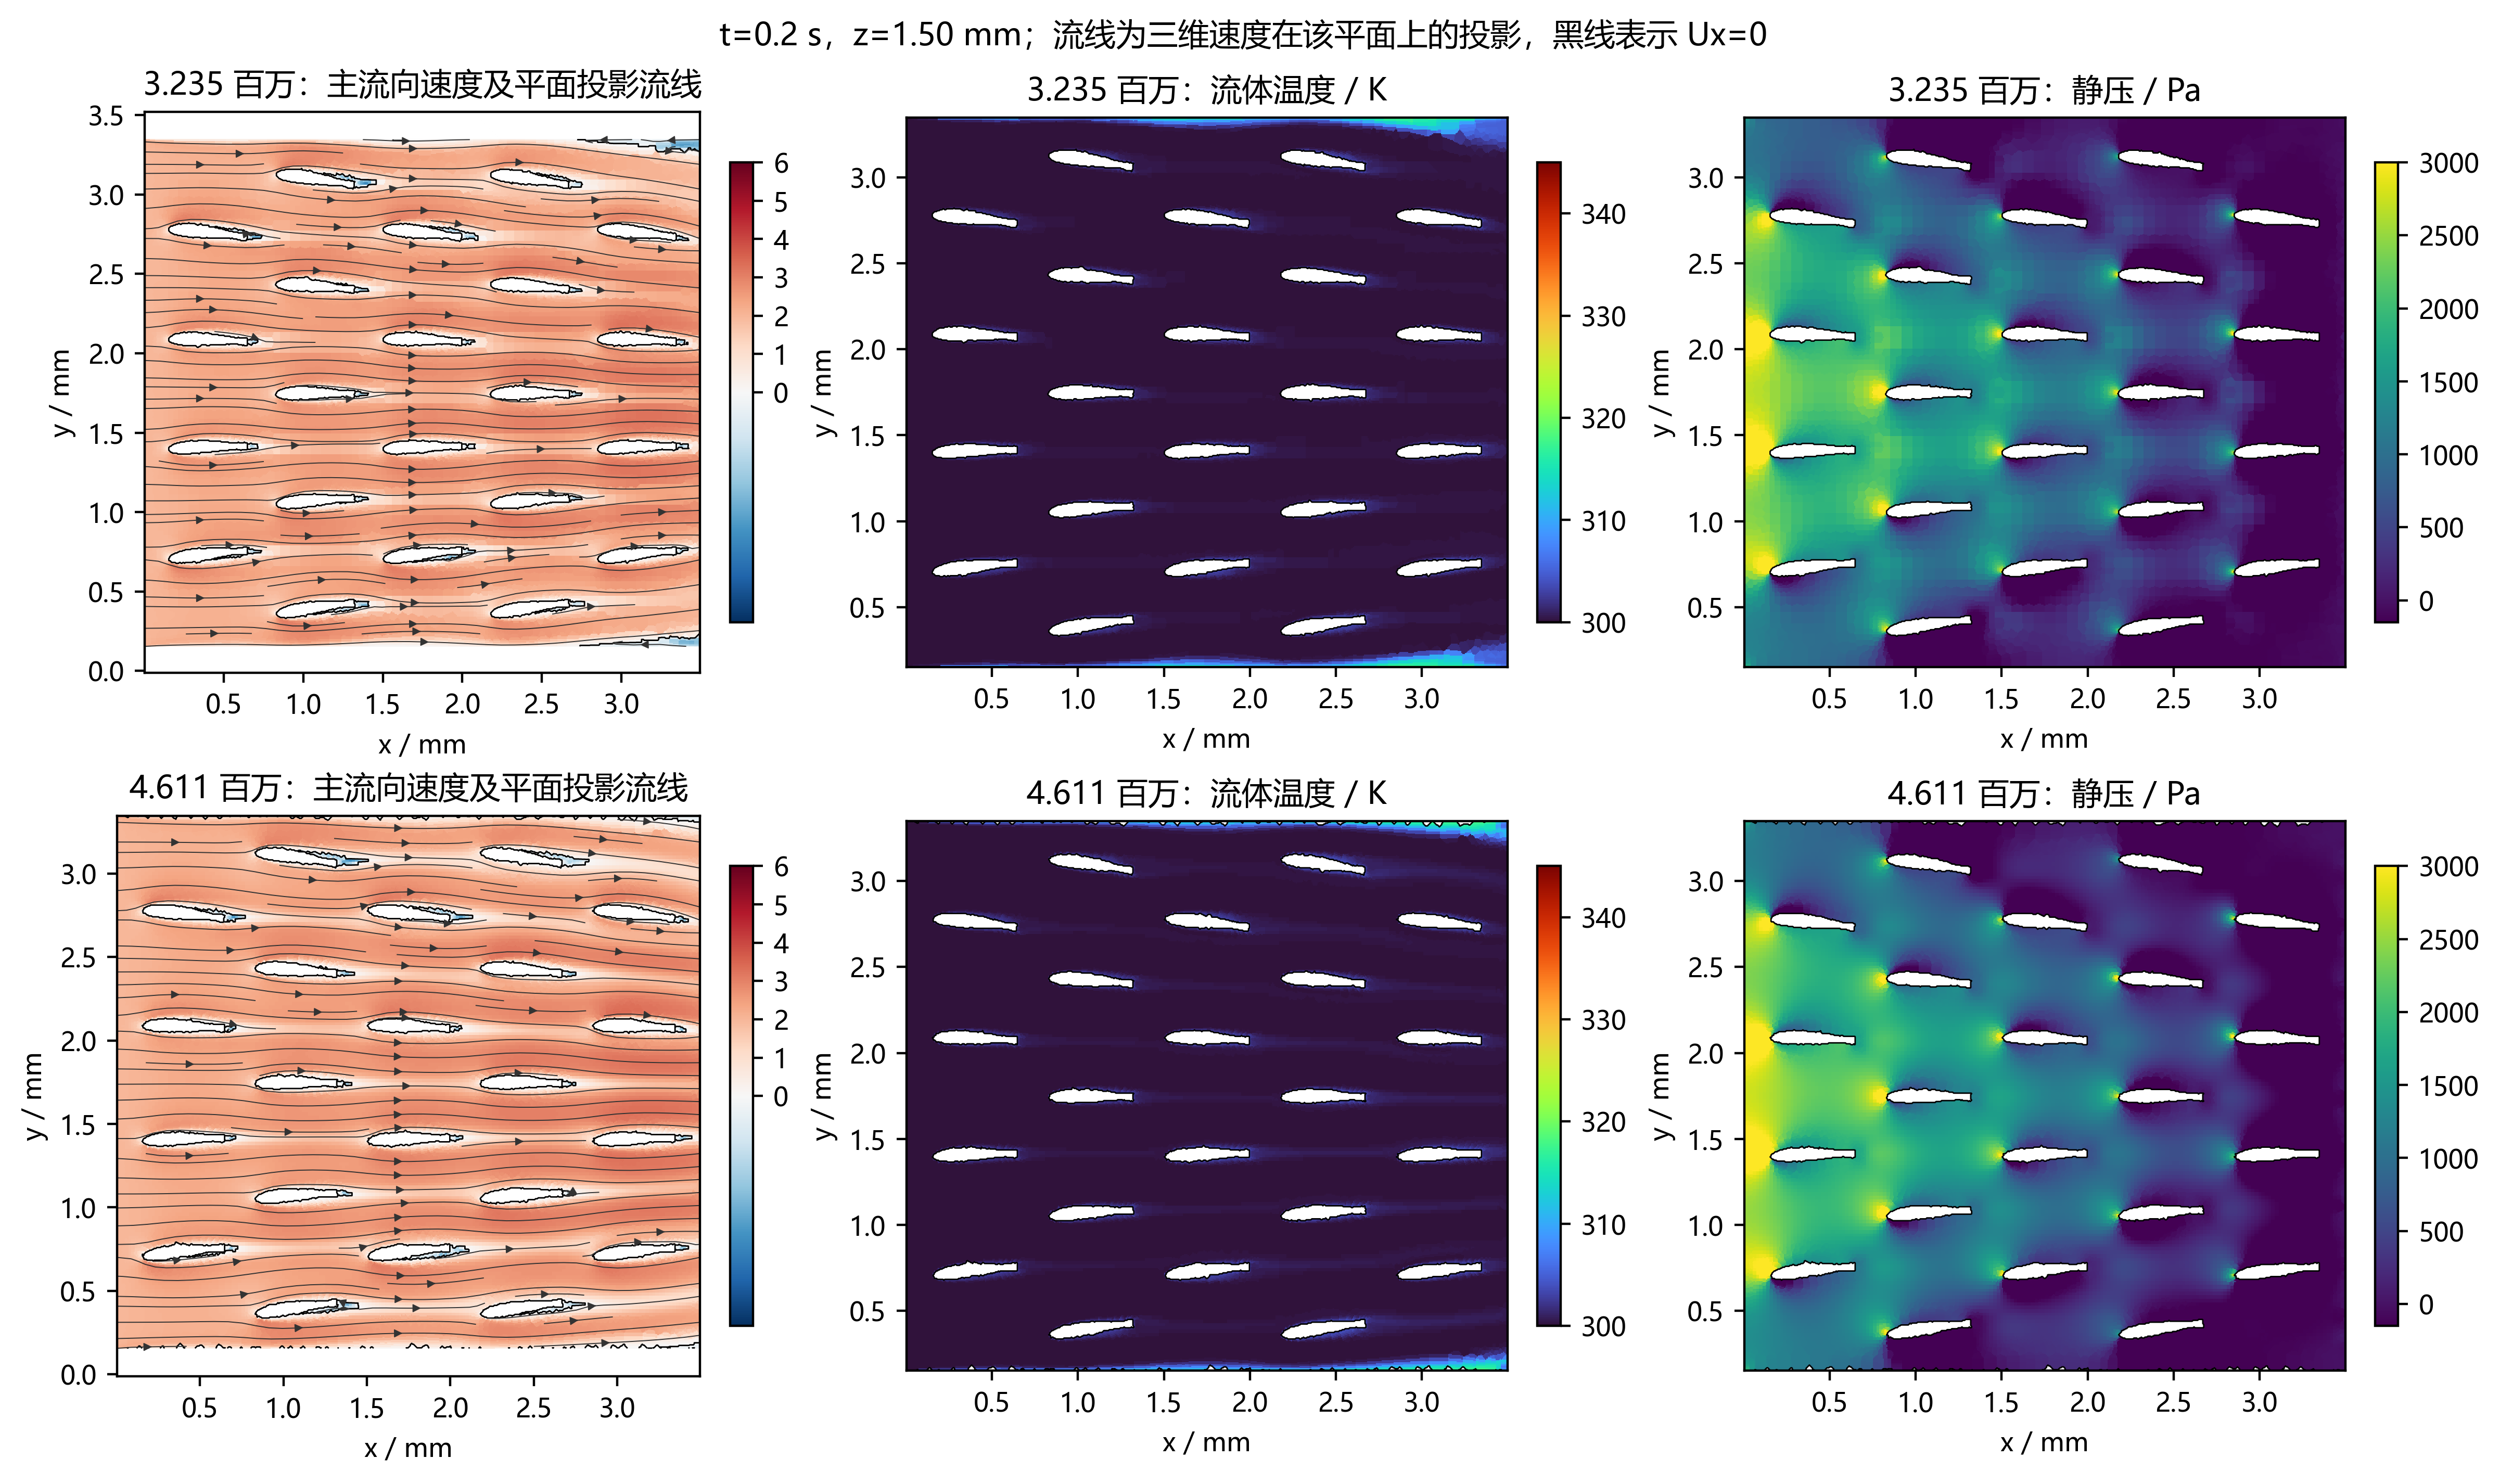
\includegraphics[width=\linewidth]{../../figs/midterm_month3_mesh_flowfield.png}
\caption{323万档（上排）与461万档（下排）的中高平面速度、投影流线、温度和静压。}\label{fig:mesh-flow}
\end{subfigure}\hfill
\begin{subfigure}{0.49\linewidth}\centering
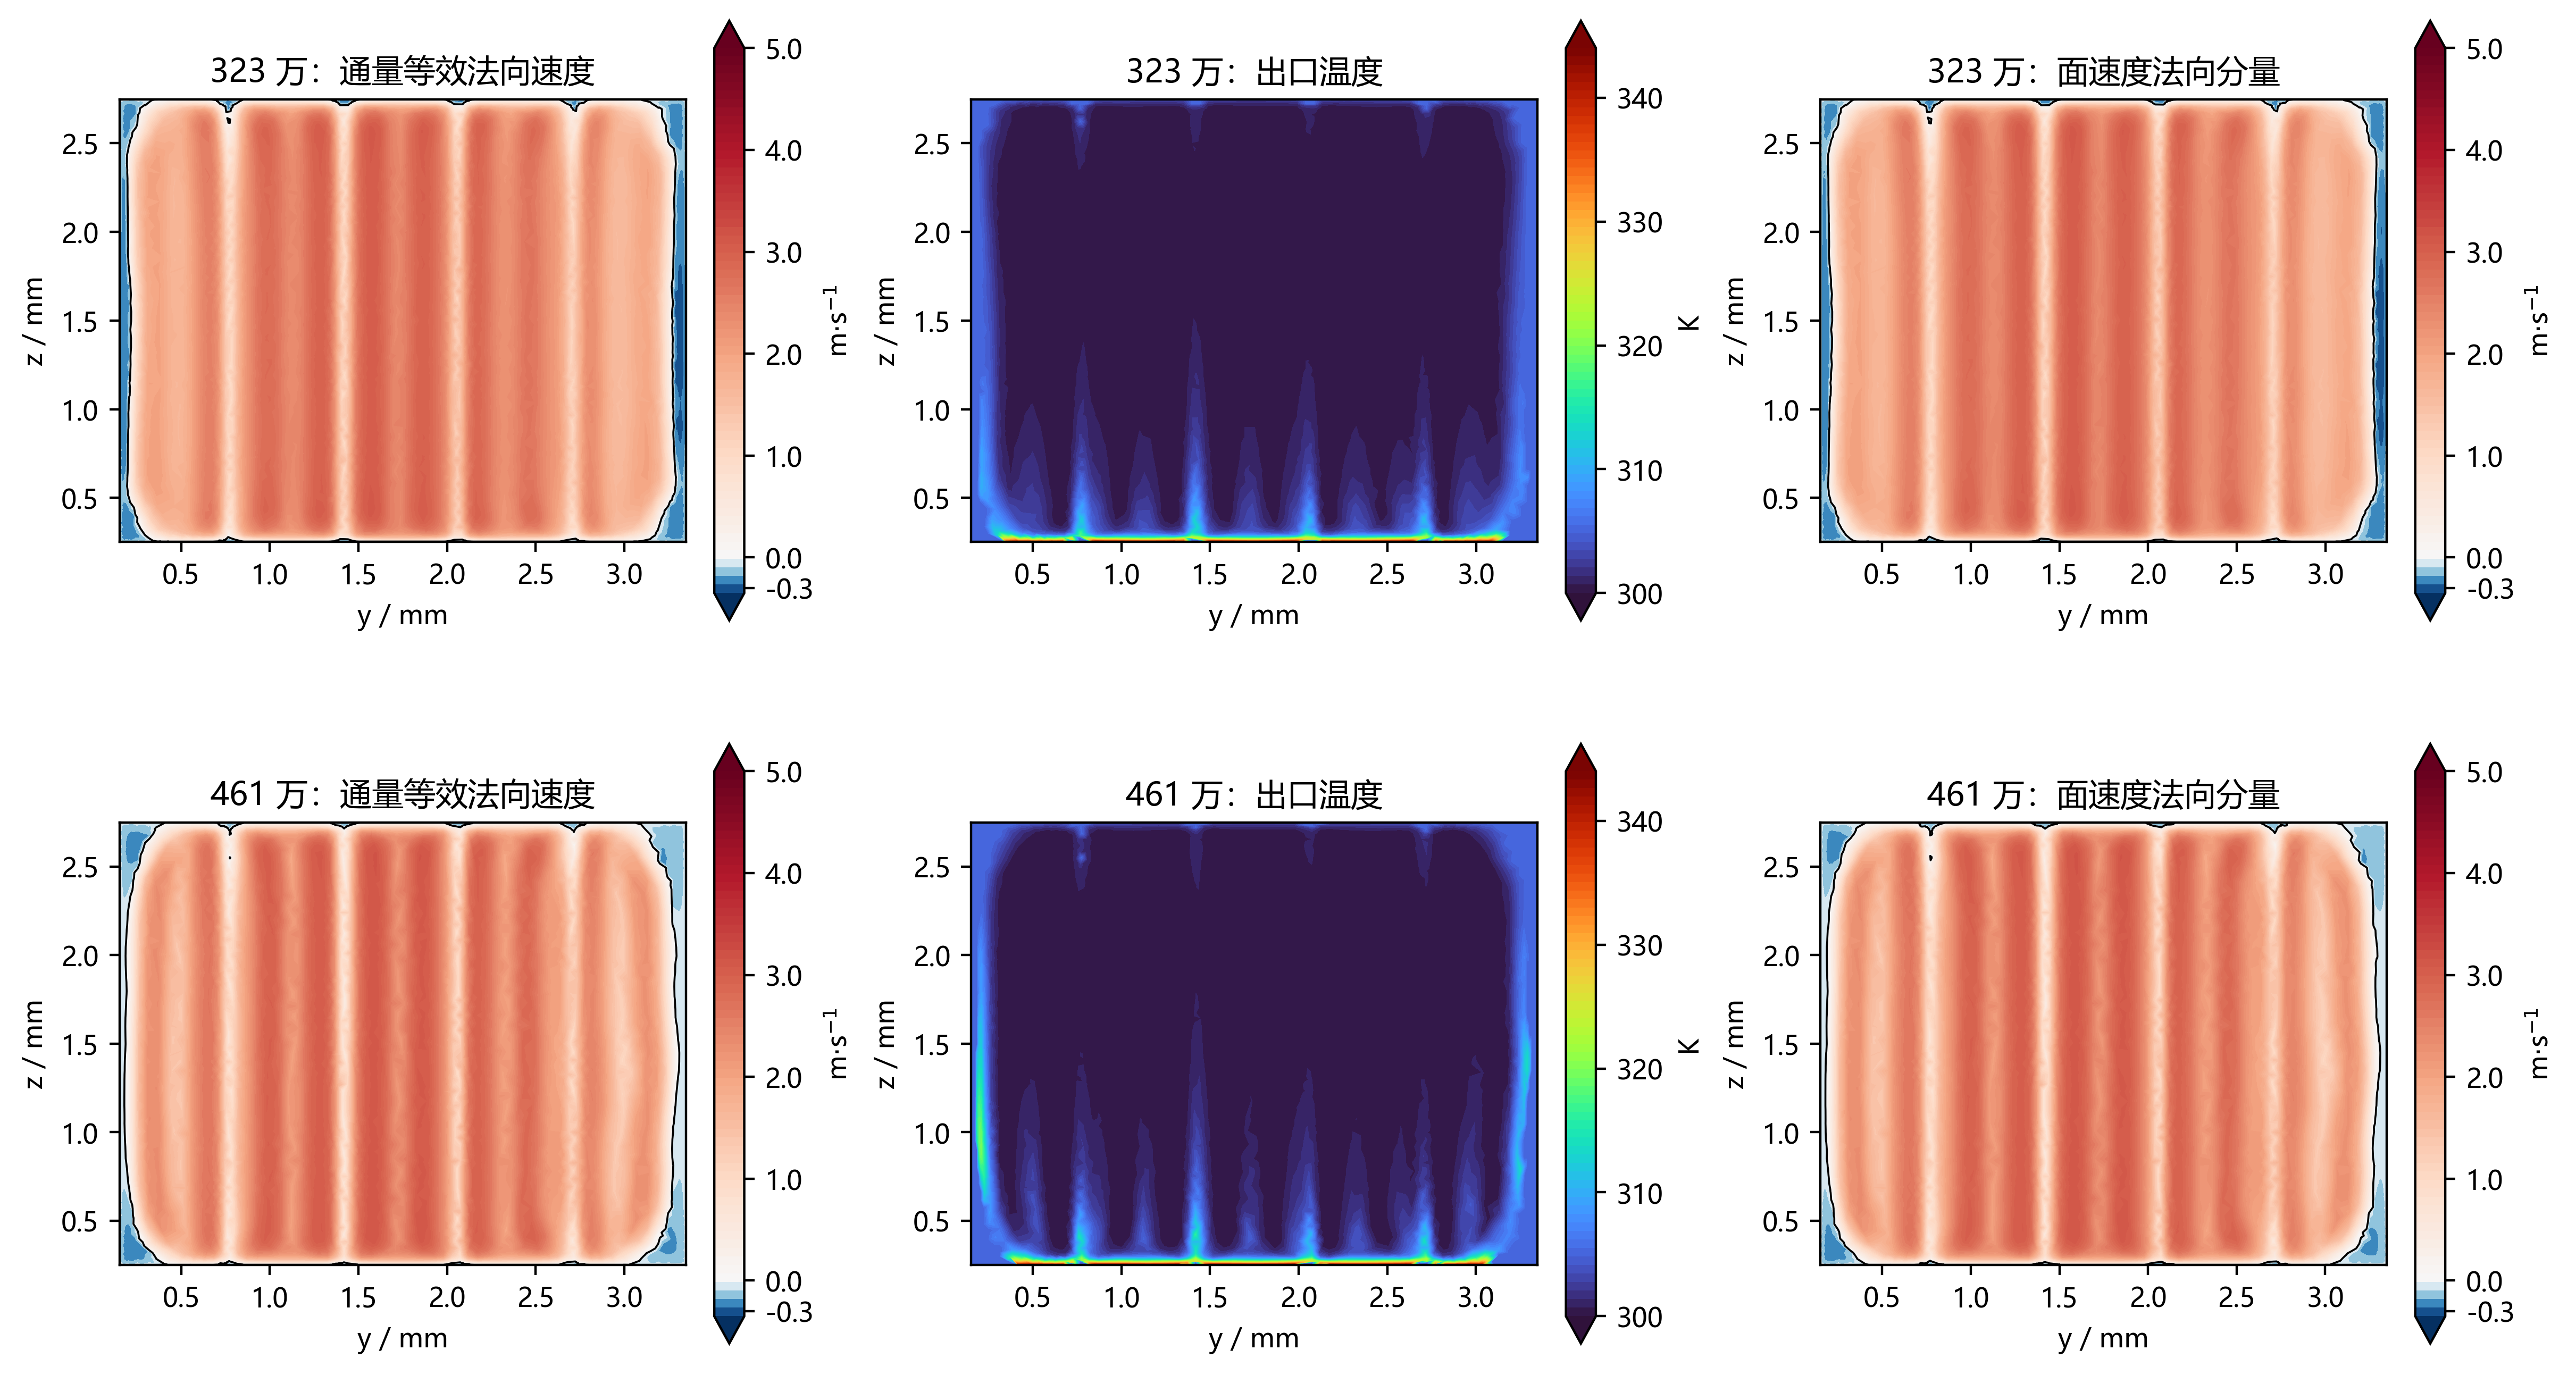
\includegraphics[width=\linewidth]{../../figs/midterm_month3_mesh_outlet.png}
\caption{323万档（上排）与461万档（下排）的出口速度和温度。出口局部回流与内部尾迹分开识别。}\label{fig:mesh-outlet}
\end{subfigure}
\caption{两种网格档的中高平面流场与出口截面}
\end{figure}
\clearpage
\setcounter{section}{3}
\setcounter{figure}{4}
\begin{figure}[!htbp]\centering
\begin{subfigure}{0.49\linewidth}\centering
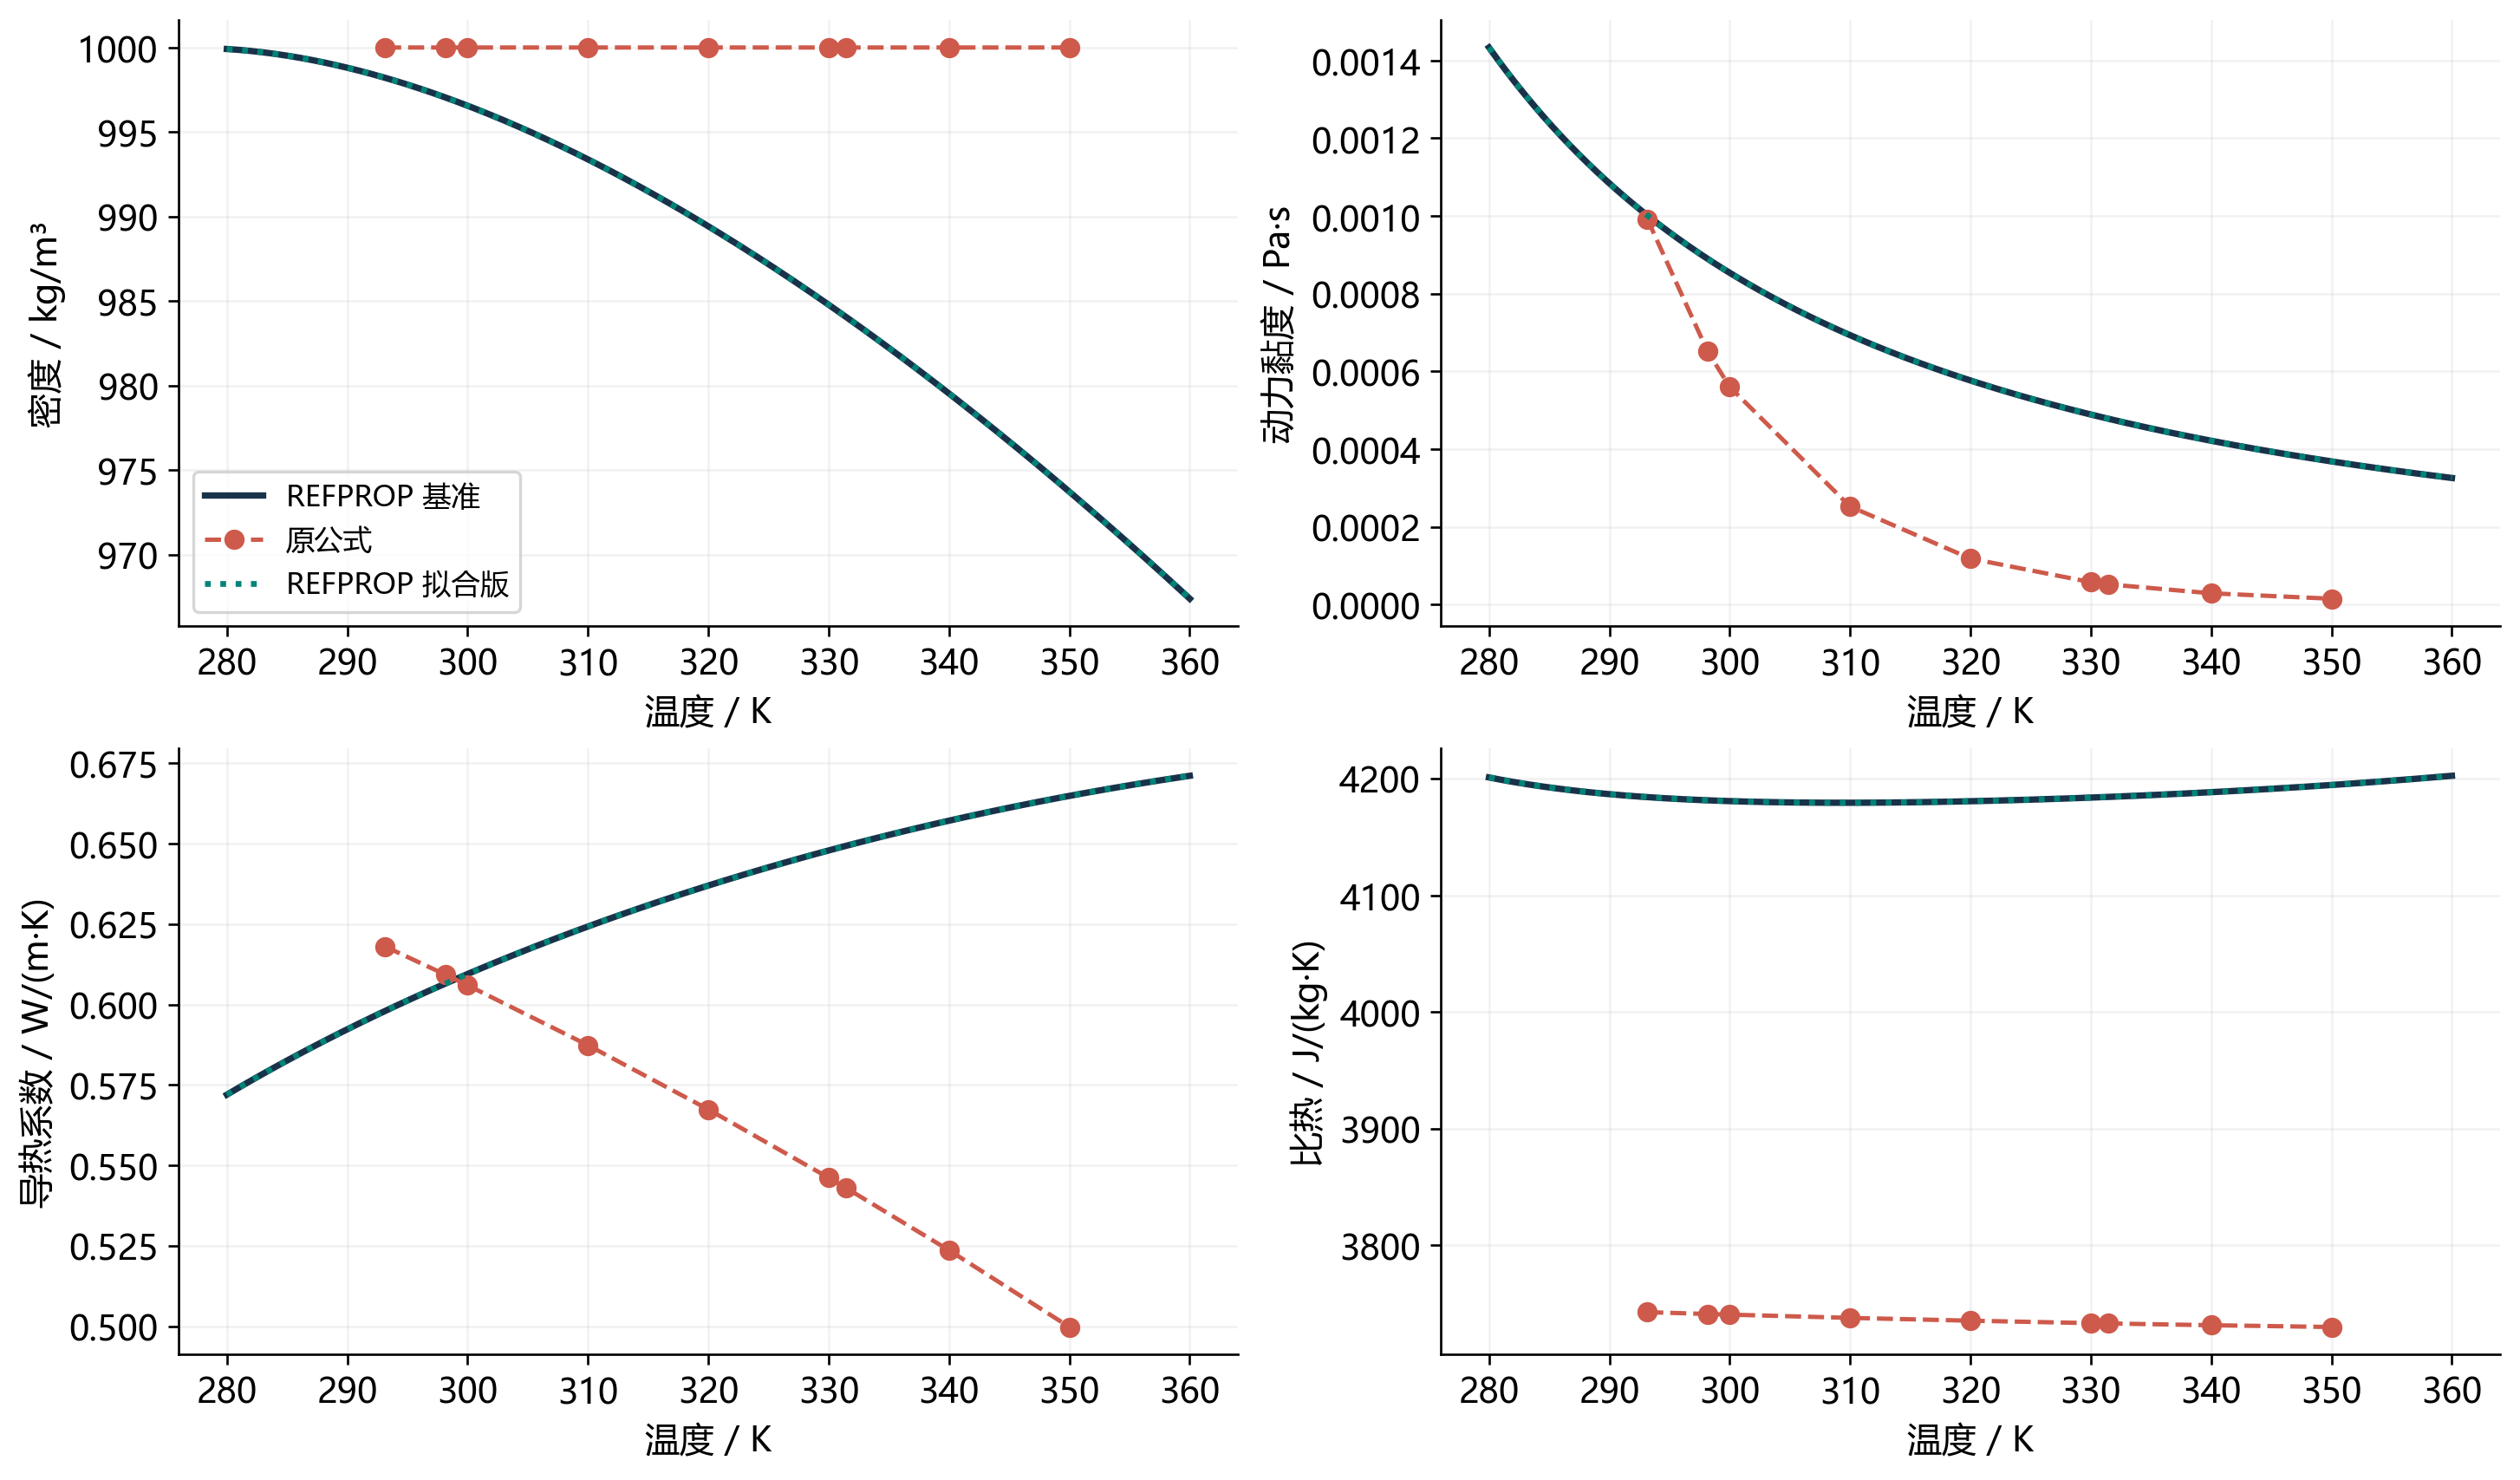
\includegraphics[width=\linewidth]{../../figs/midterm_asset_udf_01_四项物性温度曲线.png}
\caption{四项水物性随温度的变化：参考、原公式与最终REFPROP拟合版。排查候选公式与最终拟合版分别保留，不混用。}\label{fig:udf-curves}
\end{subfigure}\hfill
\begin{subfigure}{0.49\linewidth}\centering
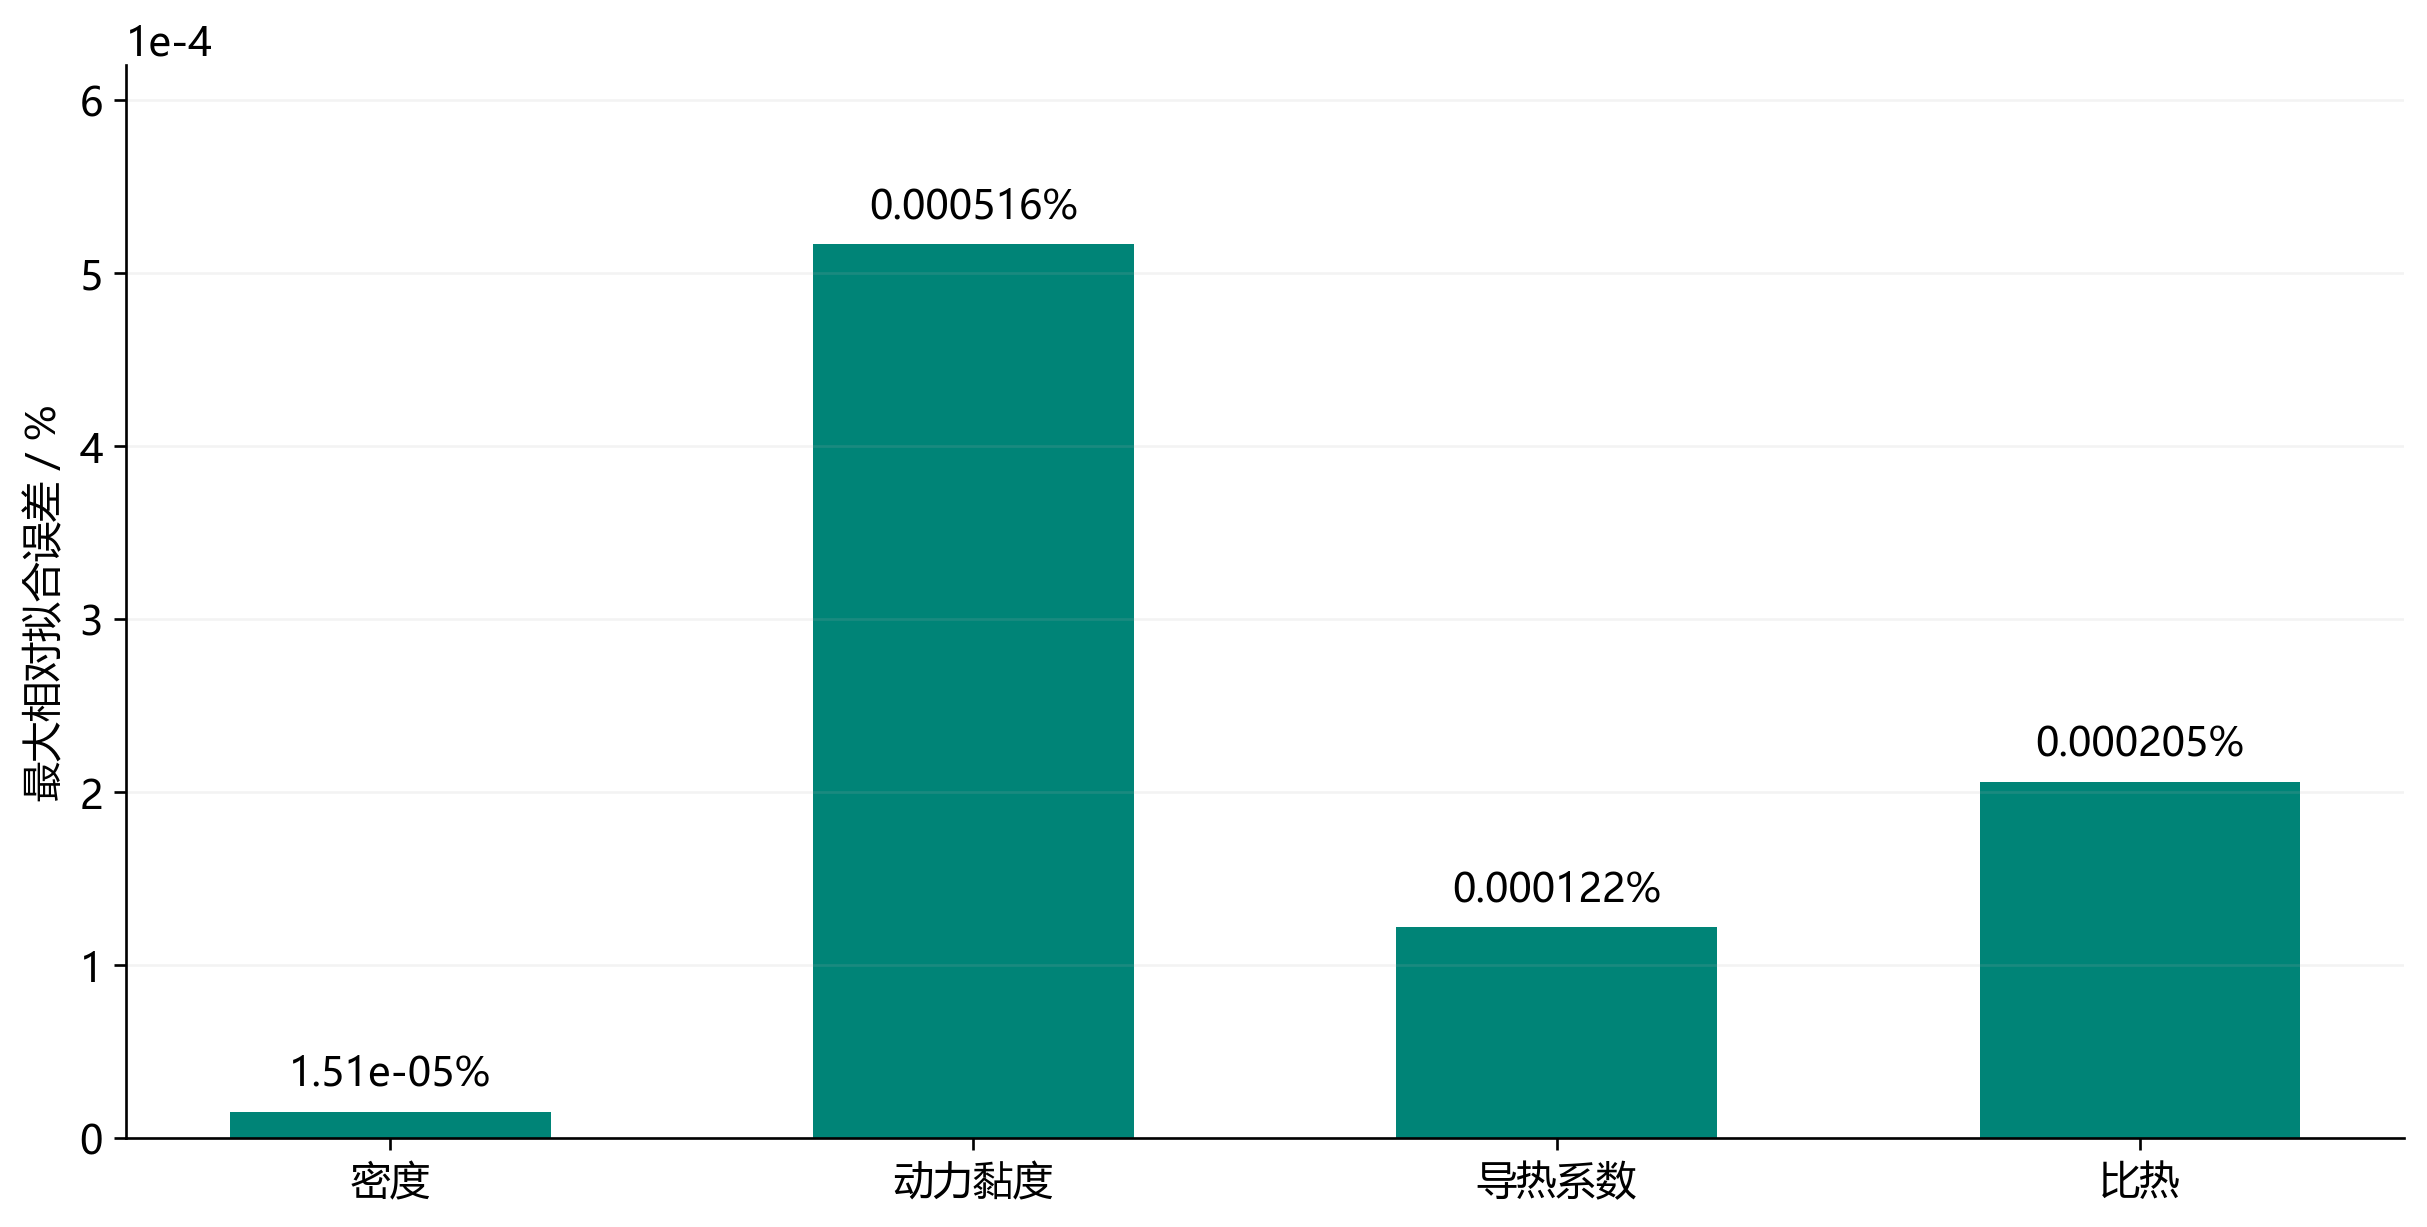
\includegraphics[width=\linewidth]{../../figs/midterm_asset_udf_03_1601点拟合误差.png}
\caption{1601温度点核对记录中的四项最大相对拟合误差。}\label{fig:udf-fit-error}
\end{subfigure}
\caption{物性随温度变化与1601点拟合误差}
\end{figure}
\clearpage
\setcounter{section}{3}
\setcounter{figure}{5}
\begin{figure}[!htbp]\centering
\begin{subfigure}{0.49\linewidth}\centering
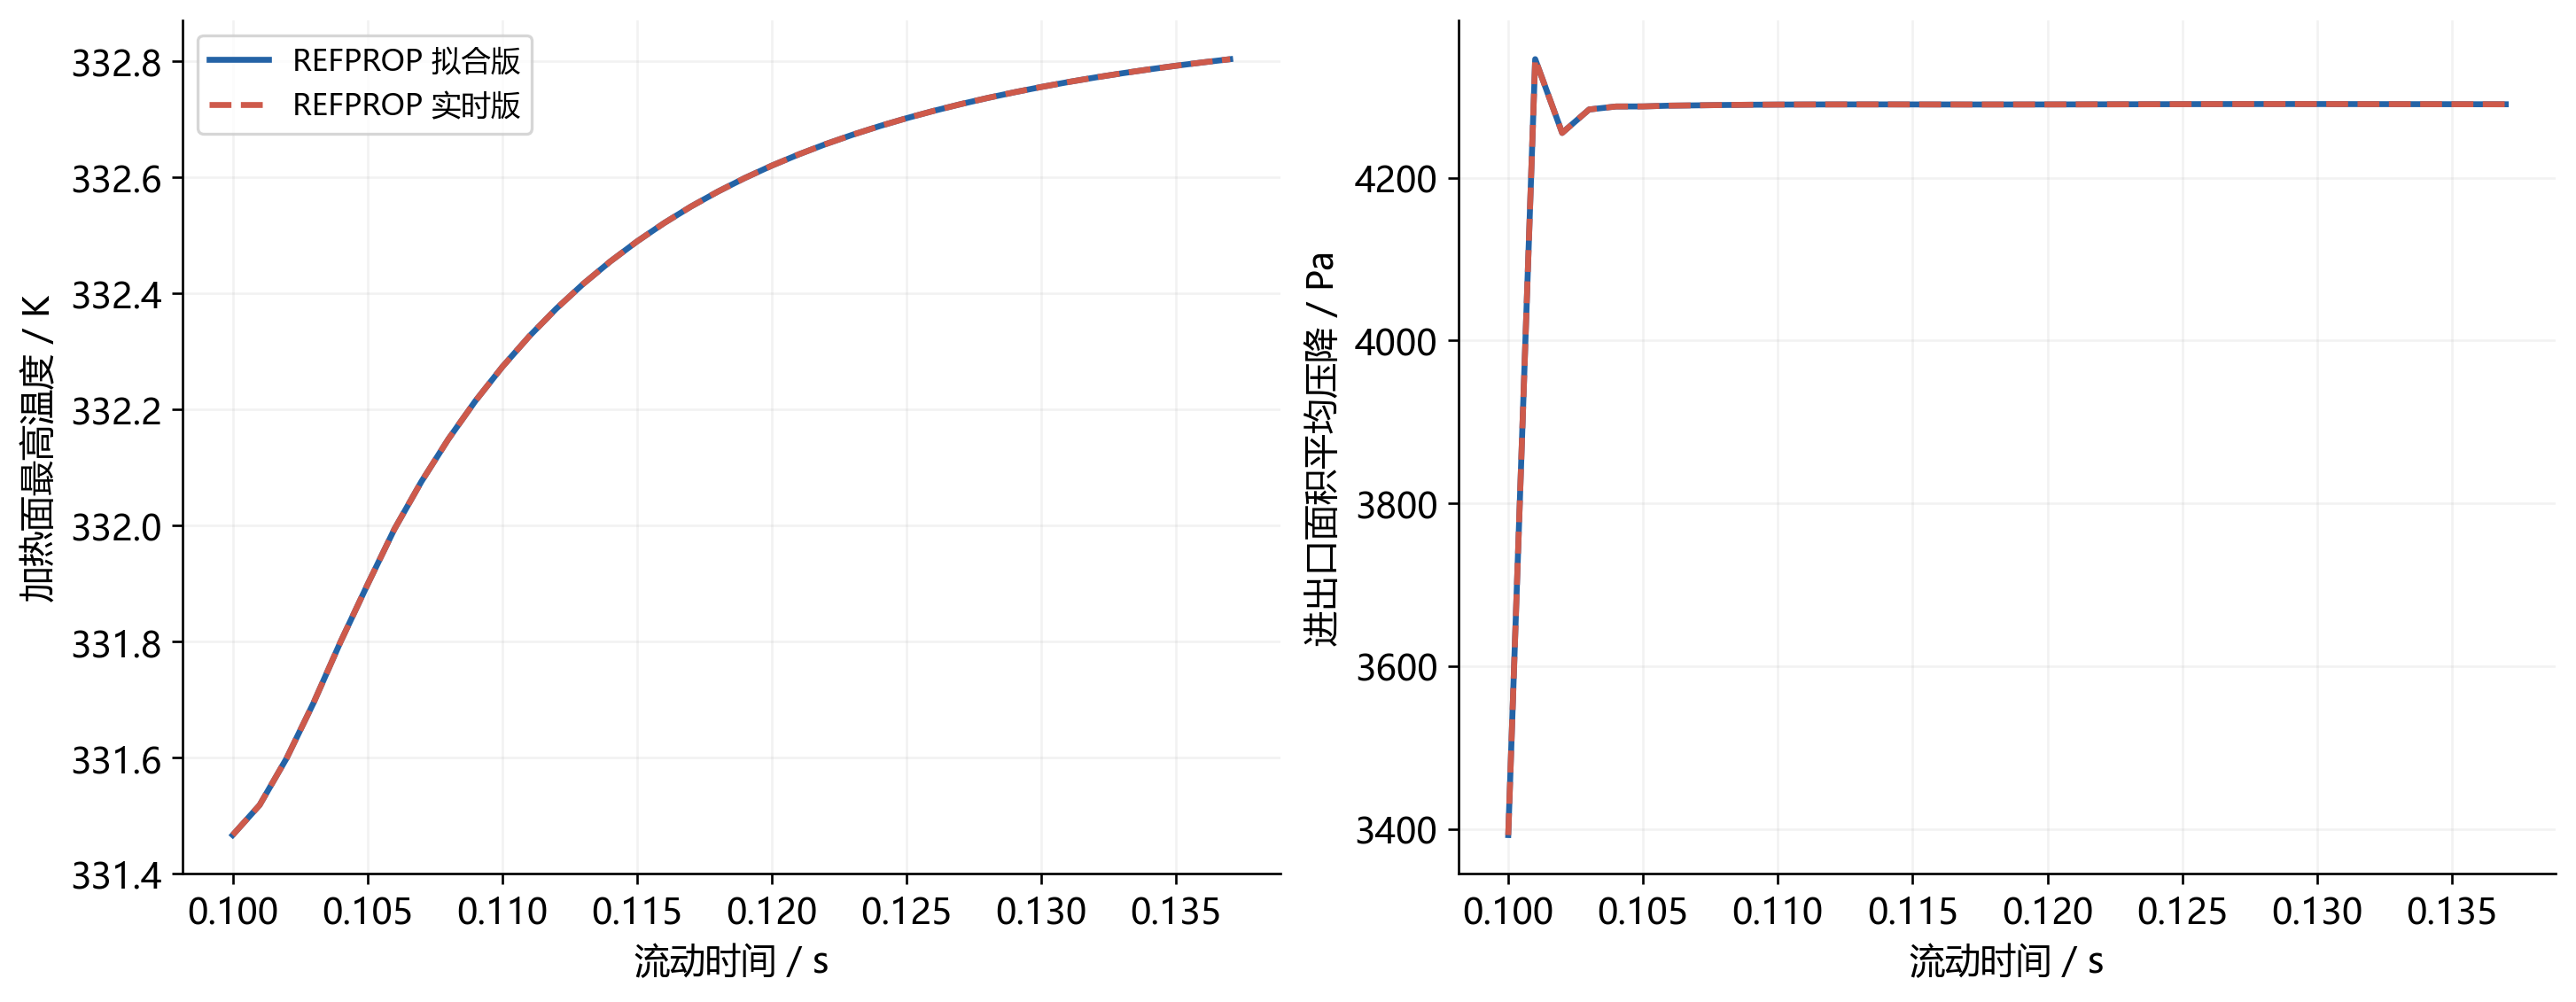
\includegraphics[width=\linewidth]{../../figs/midterm_asset_udf_04_同一时段求解结果.png}
\caption{相同初场和时间步下两种物性实现的共同时间段对照。}\label{fig:udf-common}
\end{subfigure}\hfill
\begin{subfigure}{0.49\linewidth}\centering
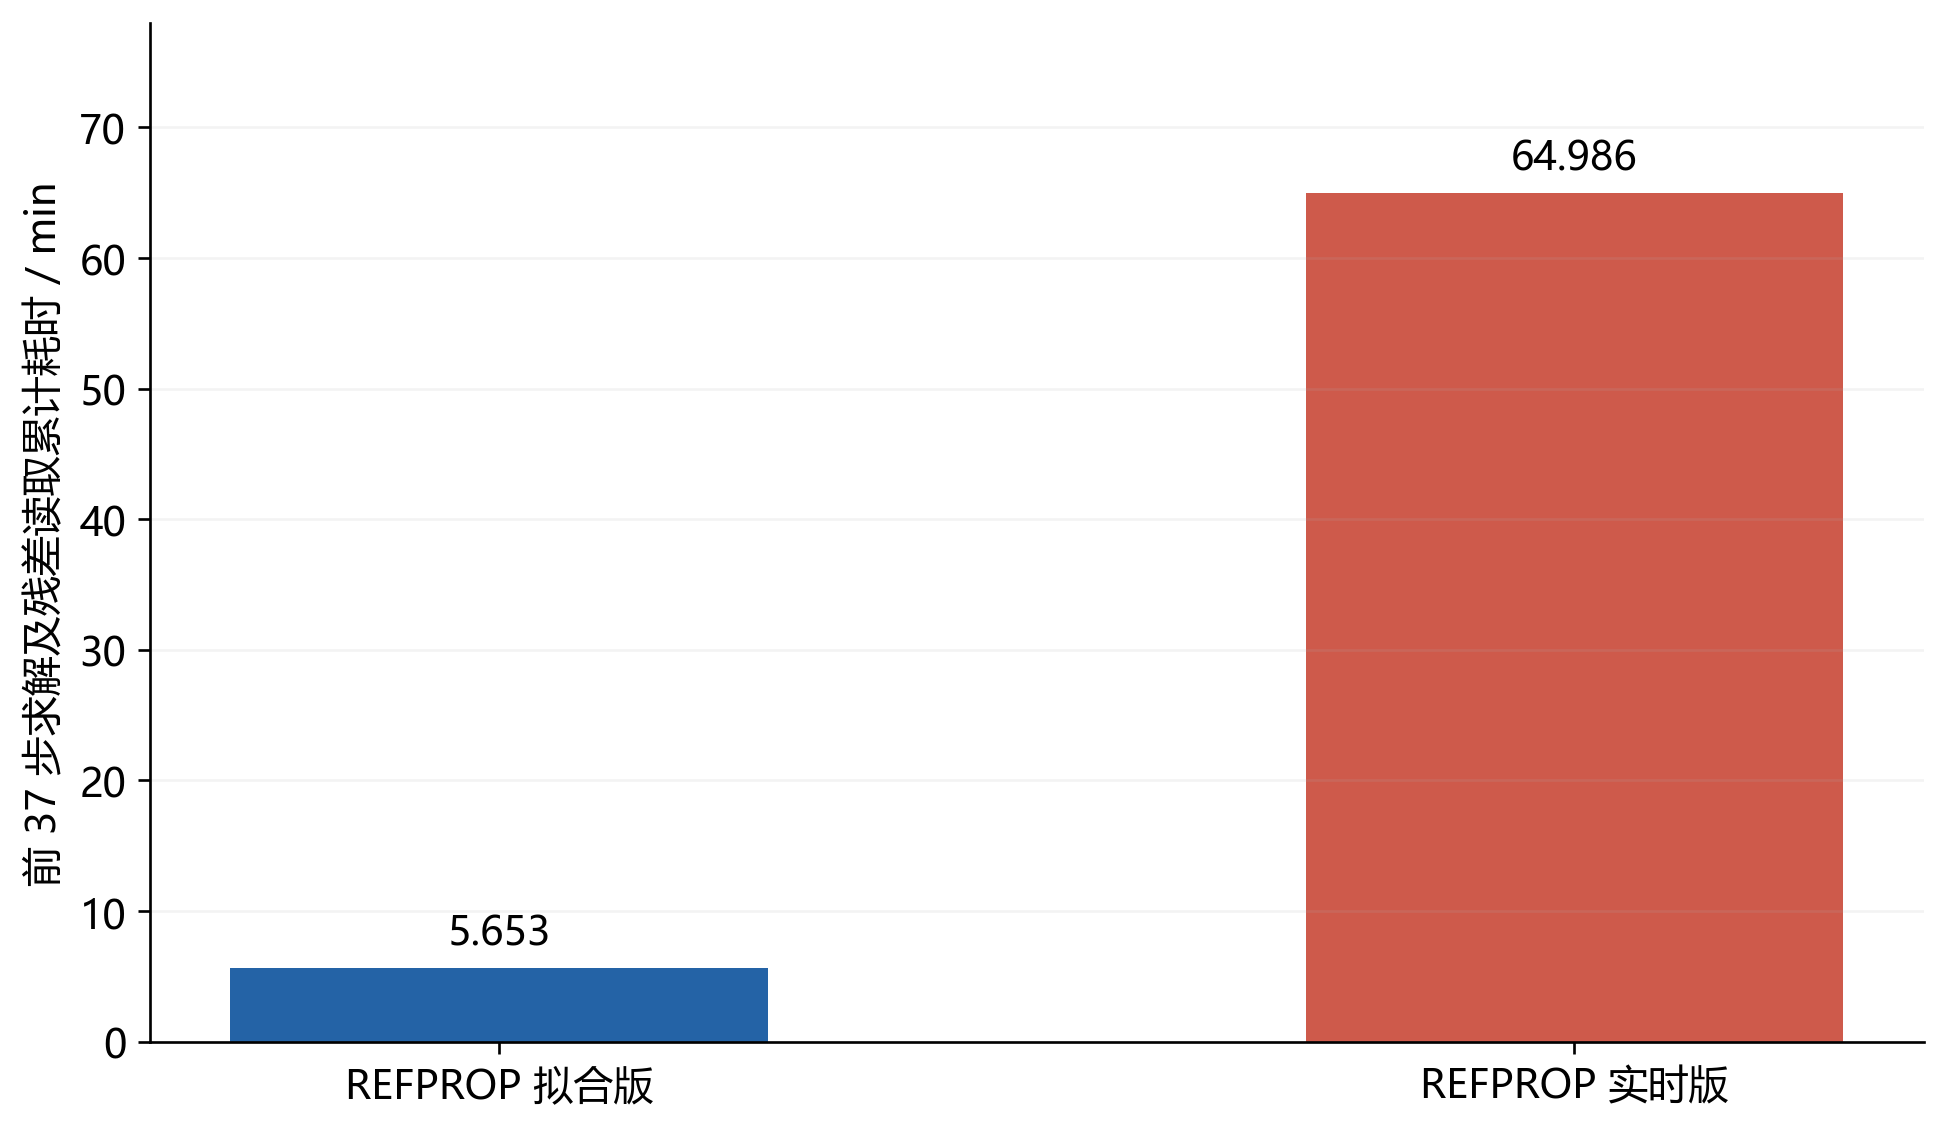
\includegraphics[width=\linewidth]{../../figs/midterm_asset_udf_05_共同37步计算耗时.png}
\caption{共同前37步的求解及残差读取耗时；不是不同总步数或代理模型的加速比较。}\label{fig:udf-time}
\end{subfigure}
\caption{两种物性实现的求解结果与计算耗时}
\end{figure}
\clearpage
\setcounter{section}{3}
\setcounter{table}{3}
\begin{table}[!htbp]
\centering
\caption{既有工况在共同热流密度下的温度与水力性能}
\label{m2:tab:results}
\begin{tabularx}{\textwidth}{@{}c Y Y Y Y Y@{}}
\toprule
\rowcolor{ydzjlight} 热流密度 & 流道 & 最高温度 & 平均温度 & 压差 & 水力功率 \\
 & & / $^\circ$C & / $^\circ$C & / kPa & / W \\
\midrule
300 & 直线 & 52.50 & 38.43 & 3.074 & 0.04919 \\
300 & 正弦 & 62.27 & 44.84 & 4.914 & 0.05897 \\
300 & NACA2416 & 72.48 & 45.99 & 0.979 & 0.01566 \\
500 & gao2.1 & 68.50 & 42.55 & 12.457 & 0.11211 \\
500 & NACA2416 & 99.60 & 56.82 & 0.926 & 0.01482 \\
\bottomrule
\end{tabularx}
\end{table}
\clearpage
\setcounter{section}{3}
\setcounter{table}{4}
\begin{table}[!htbp]
\centering
\small
\caption{非 NACA 小模型在各自保存工况下的性能}
\label{m2:tab:other-small}
\begin{tabularx}{\textwidth}{@{}Y r r r r r@{}}
\toprule
\rowcolor{ydzjlight} 模型或分支 & 热流密度 & 最高温度 & 平均温度 & 压差 & 水力功率 \\
 & / (W/cm$^2$) & / $^\circ$C & / $^\circ$C & / kPa & / W \\
\midrule
六边形 v4 & 350.00 & 45.75 & 30.77 & 512.097 & 39.45329 \\
六边形 v4.2 & 650.00 & 88.26 & 49.50 & 78.587 & 1.17881 \\
gao2.1 & 600.00 & 88.41 & 53.57 & 13.969 & 0.12572 \\
叶脉 A\_leaf & 600.00 & 61.81 & 37.92 & 47.668 & 0.76269 \\
\bottomrule
\end{tabularx}
\end{table}
\clearpage
\setcounter{section}{3}
\setcounter{table}{5}
\begin{table}[!htbp]
\centering
\small
\caption{非 NACA 小模型的网格与计算条件}
\label{m2:tab:other-conditions}
\begin{tabularx}{\textwidth}{@{}Y r r r r@{}}
\toprule
\rowcolor{ydzjlight} 模型 & 网格单元数 & 保存时刻 / s & 时间步 / s & 流量 / (mL/s) \\
\midrule
六边形 v4 & 1,443,844 & 15.00 & 0.5 & 77.043 \\
六边形 v4.2 & 1,320,229 & 6.05 & 0.01 & 15.000 \\
gao2.1 & 2,347,198 & 0.20 & 0.01 & 9.000 \\
叶脉 A\_leaf & 5,031,324 & 稳态 & --- & 16.000 \\
\bottomrule
\end{tabularx}
\end{table}
\clearpage
\setcounter{section}{3}
\setcounter{figure}{6}
\begin{figure}[!htbp]
\centering
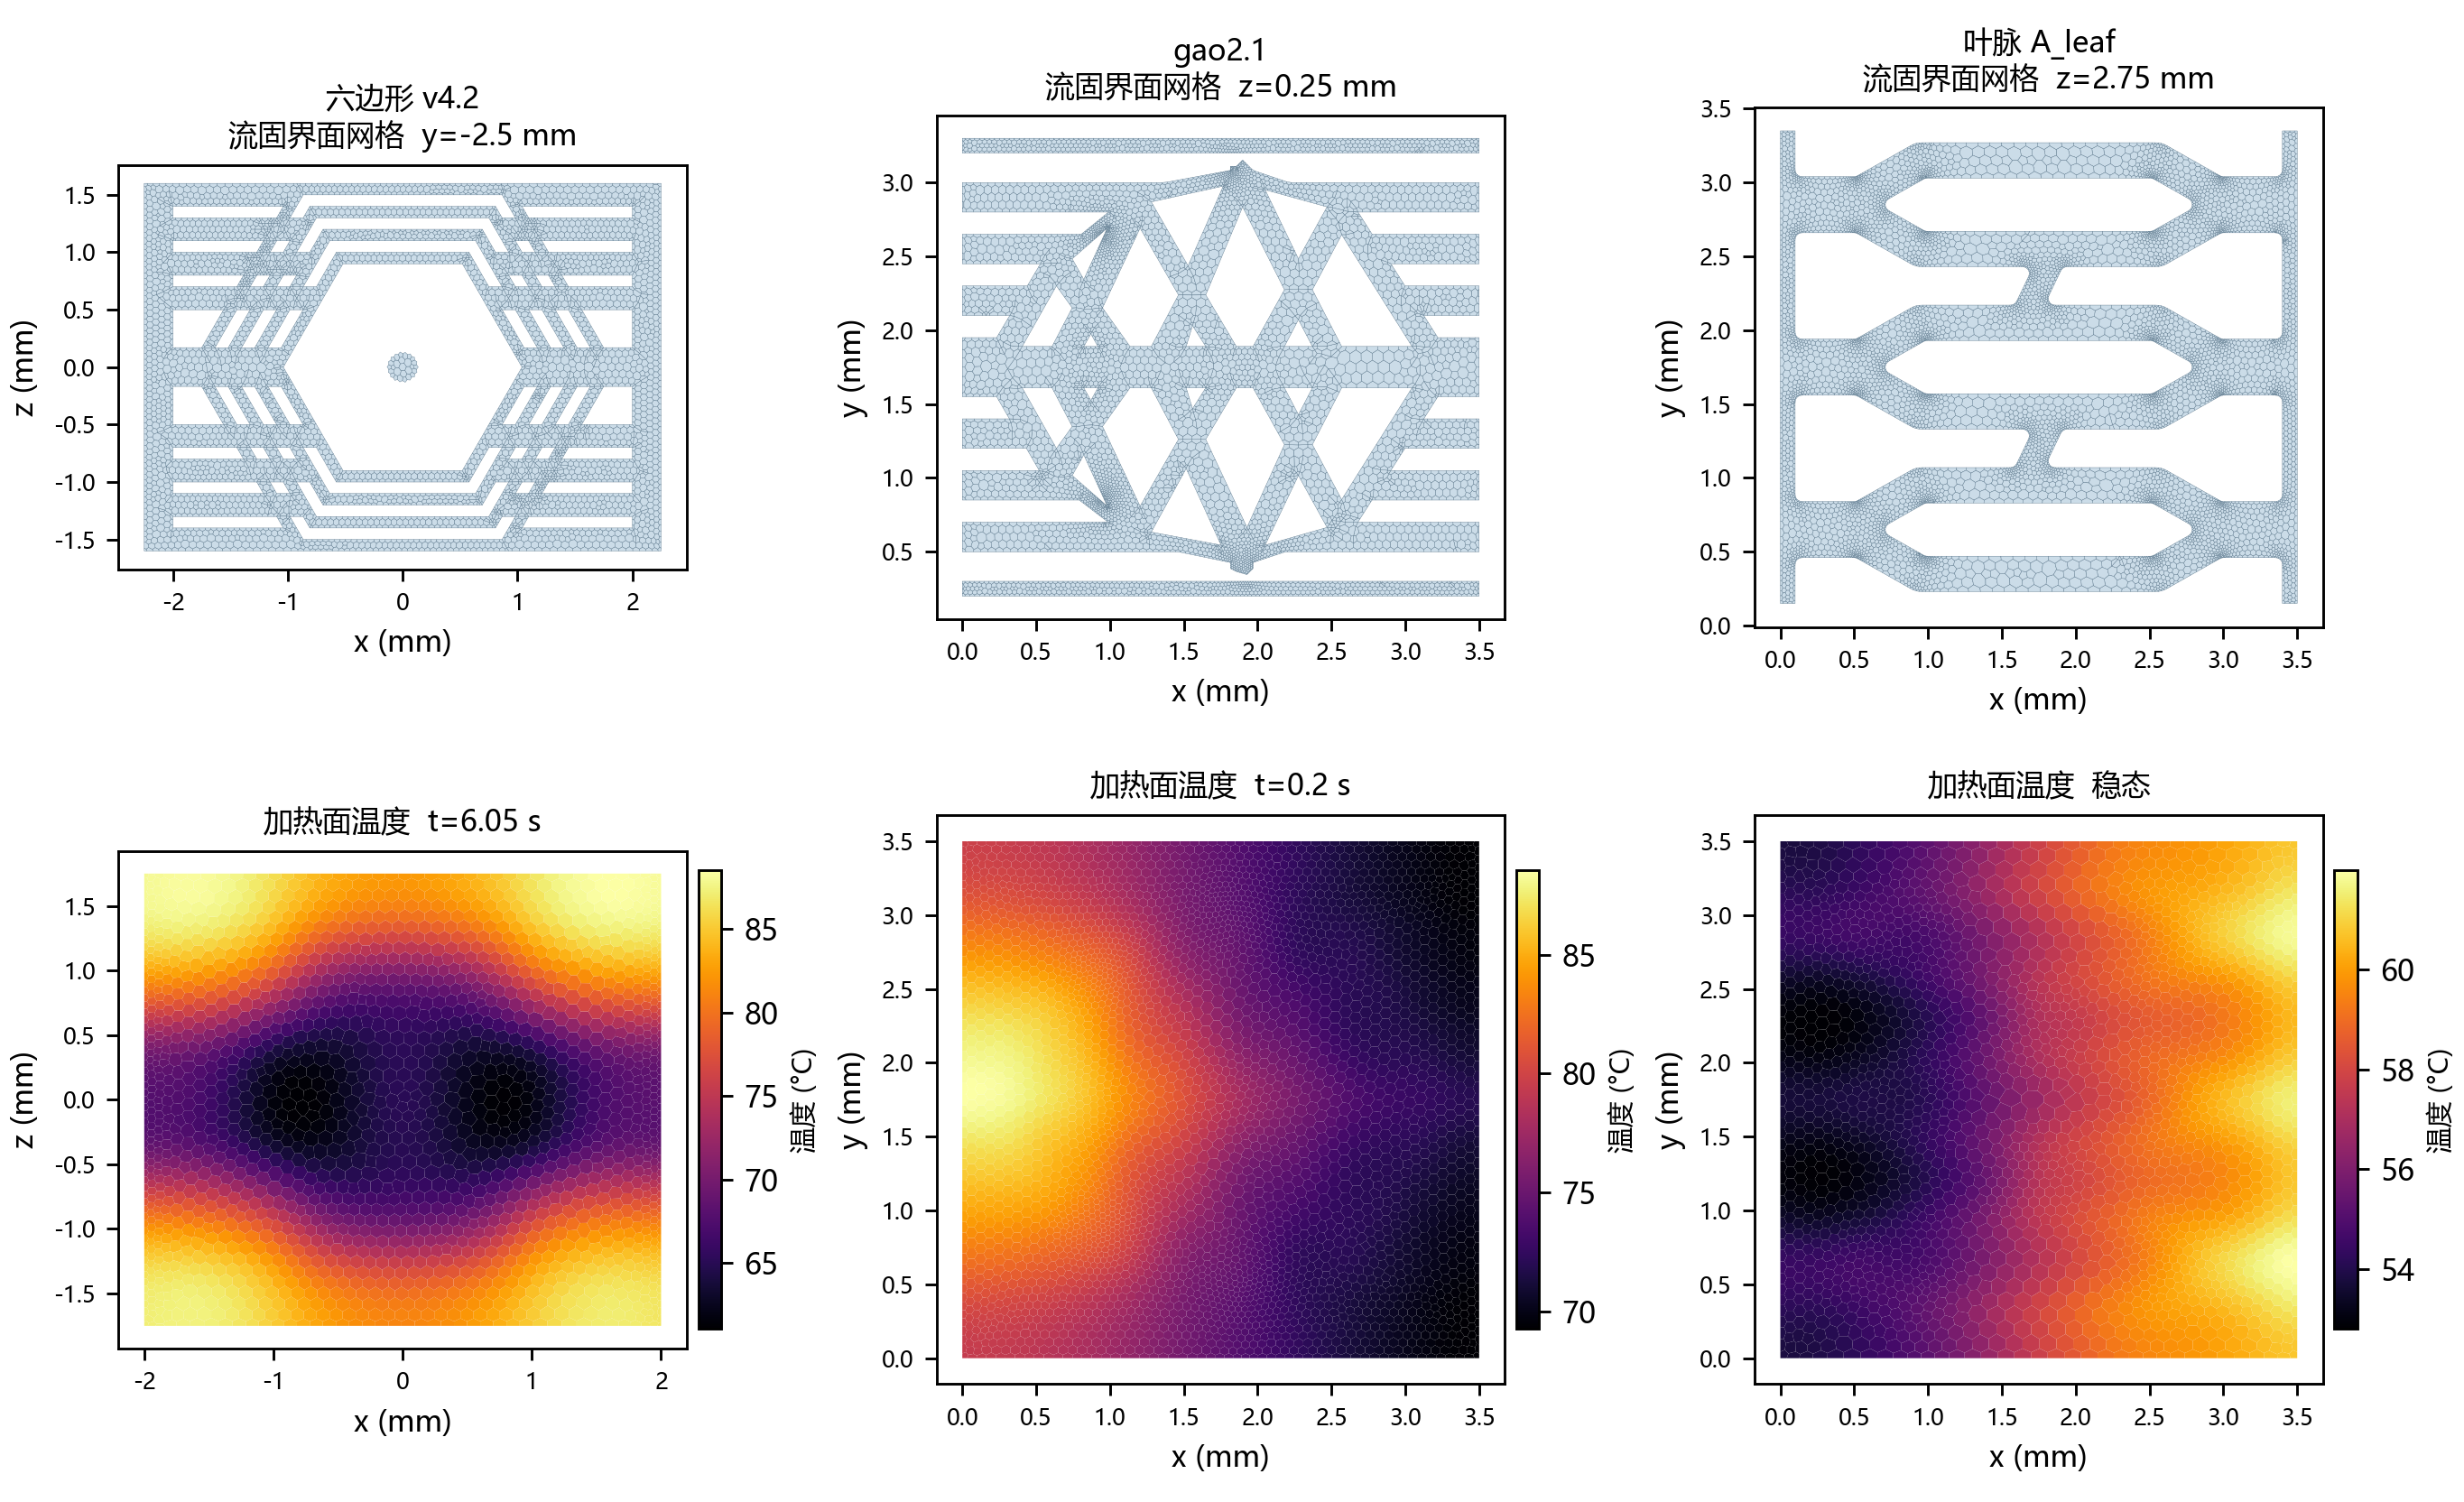
\includegraphics[width=\textwidth]{../../figs/midterm_month2_other_models.png}
\caption{六边形 v4.2、gao2.1 与叶脉模型的实际界面网格及加热面温度。上排为平面流固界面网格，下排为各自保存工况的加热面温度；各列工况不同，色标独立。}
\label{m2:fig:other-small}
\end{figure}
\clearpage
\setcounter{section}{3}
\setcounter{table}{6}
\begin{table}[!htbp]
\centering
\caption{不同翼型构型流热耦合仿真关键结果（基准工况）}
\label{m2:tab:airfoil}
\begin{tabularx}{\textwidth}{@{}l c c c c@{}}
\toprule
\rowcolor{ydzjlight} 构型 & 最高温度 / K & 底板平均温度 / K & $h$ / (W/(m$^2$·K)) & PEC \\
\midrule
NACA0015 & 357.9 & 356.1 & 756.6 & 1.00 \\
NACA0021 & 355.7 & 354.0 & 765.3 & 1.10 \\
NACA0024 & 354.9 & 353.2 & 798.5 & 1.19 \\
NACA4424 & 354.4 & 352.7 & 789.8 & 1.21 \\
NACA6424 & 358.1 & 356.3 & 750.5 & 1.00 \\
NACA6624 & 357.9 & 356.1 & 750.2 & 1.01 \\
\bottomrule
\end{tabularx}
\end{table}
\clearpage
\setcounter{section}{3}
\setcounter{table}{7}
\begin{table}[!htbp]
\centering
\small
\caption{350 W/cm$^2$ 下 NACA 小模型的保存结果}
\label{m2:tab:naca350}
\begin{tabularx}{\textwidth}{@{}Y r r r r r@{}}
\toprule
\rowcolor{ydzjlight} 模型或分支 & 热流密度 & 最高温度 & 平均温度 & 压差 & 水力功率 \\
 & / (W/cm$^2$) & / $^\circ$C & / $^\circ$C & / kPa & / W \\
\midrule
0016 A06 基础 & 350.00 & 58.20 & 34.18 & 3.393 & 0.05428 \\
2416 A00 core & 350.00 & 71.03 & 40.07 & 2.456 & 0.03929 \\
2416 A00 尾部 BOI & 350.00 & 71.01 & 39.25 & 2.512 & 0.04019 \\
0016 A06 拟合物性 & 350.00 & 59.61 & 34.62 & 4.290 & 0.06864 \\
0016 A06 REFPROP & 350.00 & 59.54 & 34.59 & 4.290 & 0.06864 \\
2416 v3 & 350.00 & 72.83 & 38.74 & 2.348 & 0.03757 \\
\bottomrule
\end{tabularx}
\end{table}
\clearpage
\setcounter{section}{3}
\setcounter{table}{8}
\begin{table}[!htbp]
\centering
\small
\caption{同热负荷、同流量与同保存时刻的 v2 翼型结果}
\label{m2:tab:nacav2}
\begin{tabularx}{\textwidth}{@{}Y r r r r r@{}}
\toprule
\rowcolor{ydzjlight} 模型或分支 & 热流密度 & 最高温度 & 平均温度 & 压差 & 水力功率 \\
 & / (W/cm$^2$) & / $^\circ$C & / $^\circ$C & / kPa & / W \\
\midrule
NACA0016 v2 & 450.00 & 85.34 & 43.21 & 2.248 & 0.03596 \\
NACA1416 v2 & 450.00 & 85.31 & 43.46 & 2.255 & 0.03609 \\
NACA3416 v2 & 450.00 & 85.11 & 43.12 & 2.366 & 0.03785 \\
\bottomrule
\end{tabularx}
\end{table}
\clearpage
\setcounter{section}{3}
\setcounter{figure}{7}
\begin{figure}[!htbp]
\centering
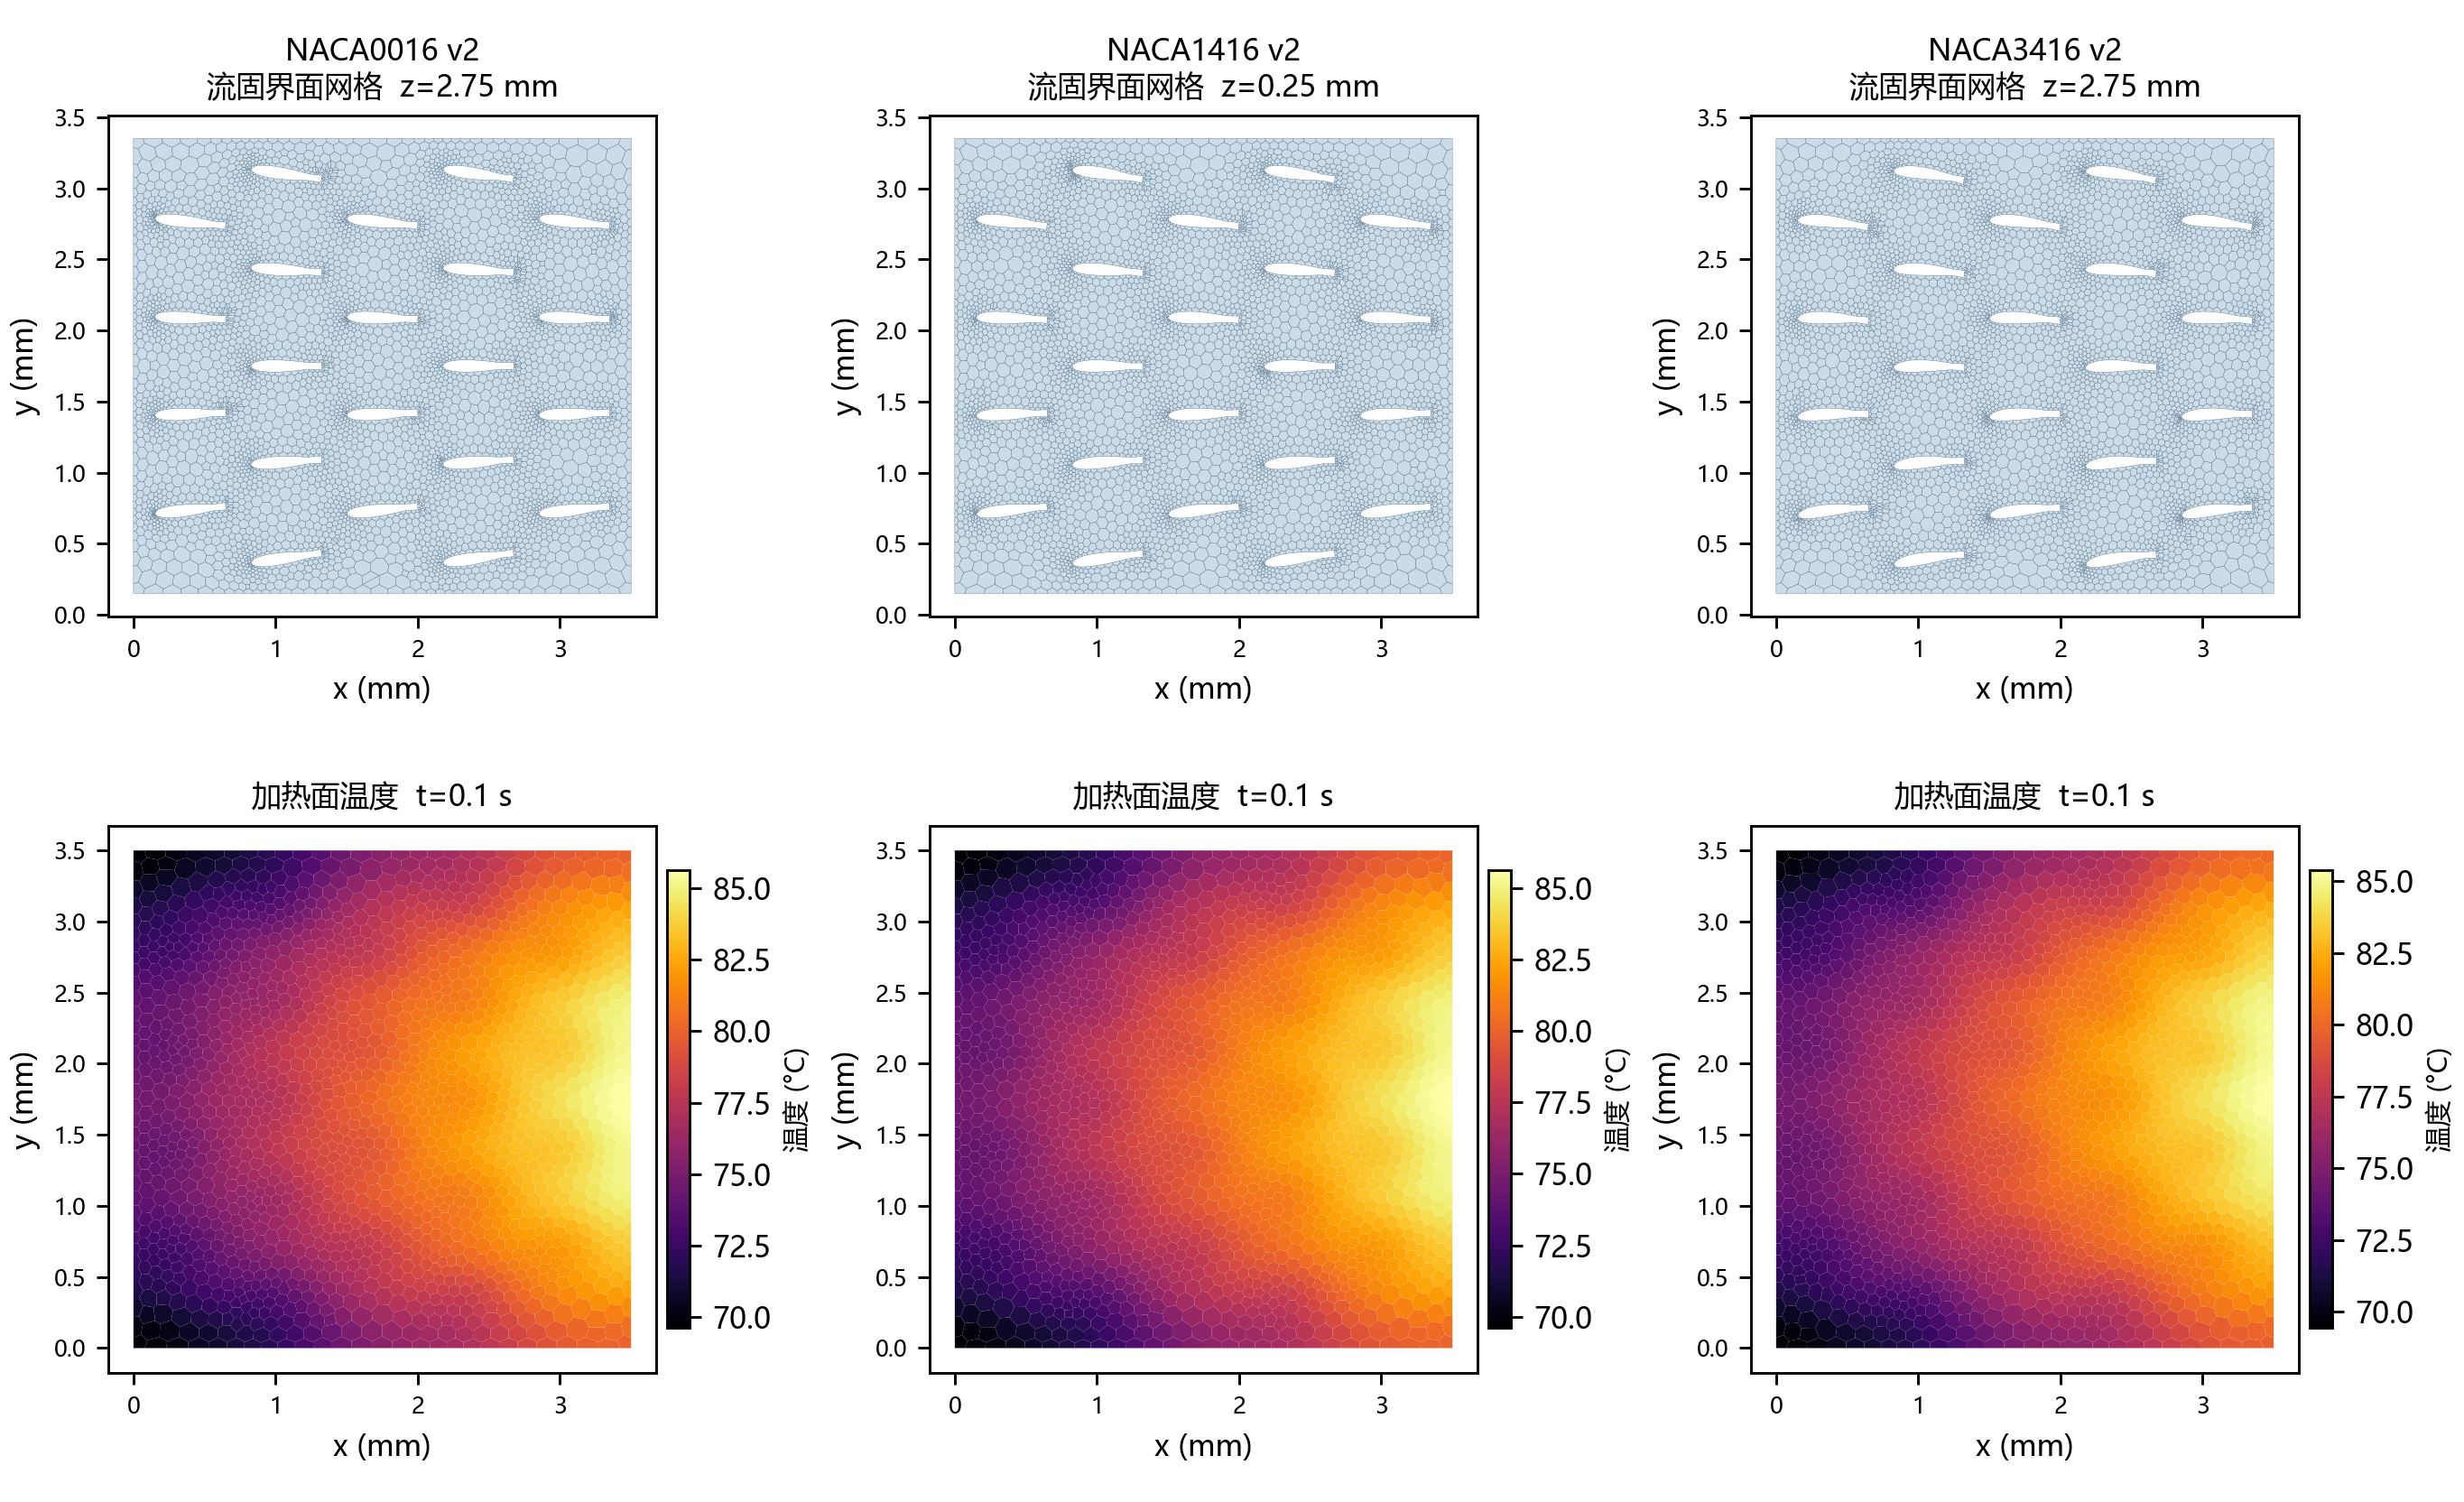
\includegraphics[width=\textwidth]{../../figs/midterm_month2_naca_models.png}
\caption{NACA0016、1416、3416 v2 小模型的界面网格与 0.10 s 加热面温度。上排为实际平面流固界面网格，下排温度来自各自配套 Data 文件，色标独立。}
\label{m2:fig:naca-small}
\end{figure}
\clearpage
\setcounter{section}{3}
\setcounter{table}{9}
\begin{table}[!htbp]
\centering
\small
\caption{NACA2420 在 1 s 时刻的设置与时间步验证结果}
\label{m2:tab:naca2420}
\begin{tabularx}{\textwidth}{@{}Y r r r r r@{}}
\toprule
\rowcolor{ydzjlight} 模型或分支 & 热流密度 & 最高温度 & 平均温度 & 压差 & 水力功率 \\
 & / (W/cm$^2$) & / $^\circ$C & / $^\circ$C & / kPa & / W \\
\midrule
2420 v4 原始 & 126.82 & 43.08 & 31.40 & 1.377 & 0.01653 \\
2420 回流 300 K & 126.82 & 44.23 & 31.83 & 1.651 & 0.01988 \\
2420 IAPWS $\Delta t=0.01$ s & 126.82 & 44.32 & 31.87 & 1.652 & 0.01989 \\
2420 IAPWS $\Delta t=0.005$ s & 126.82 & 44.32 & 31.87 & 1.652 & 0.01989 \\
\bottomrule
\end{tabularx}
\end{table}
\clearpage
\setcounter{section}{3}
\setcounter{figure}{8}
\begin{figure}[!htbp]\centering
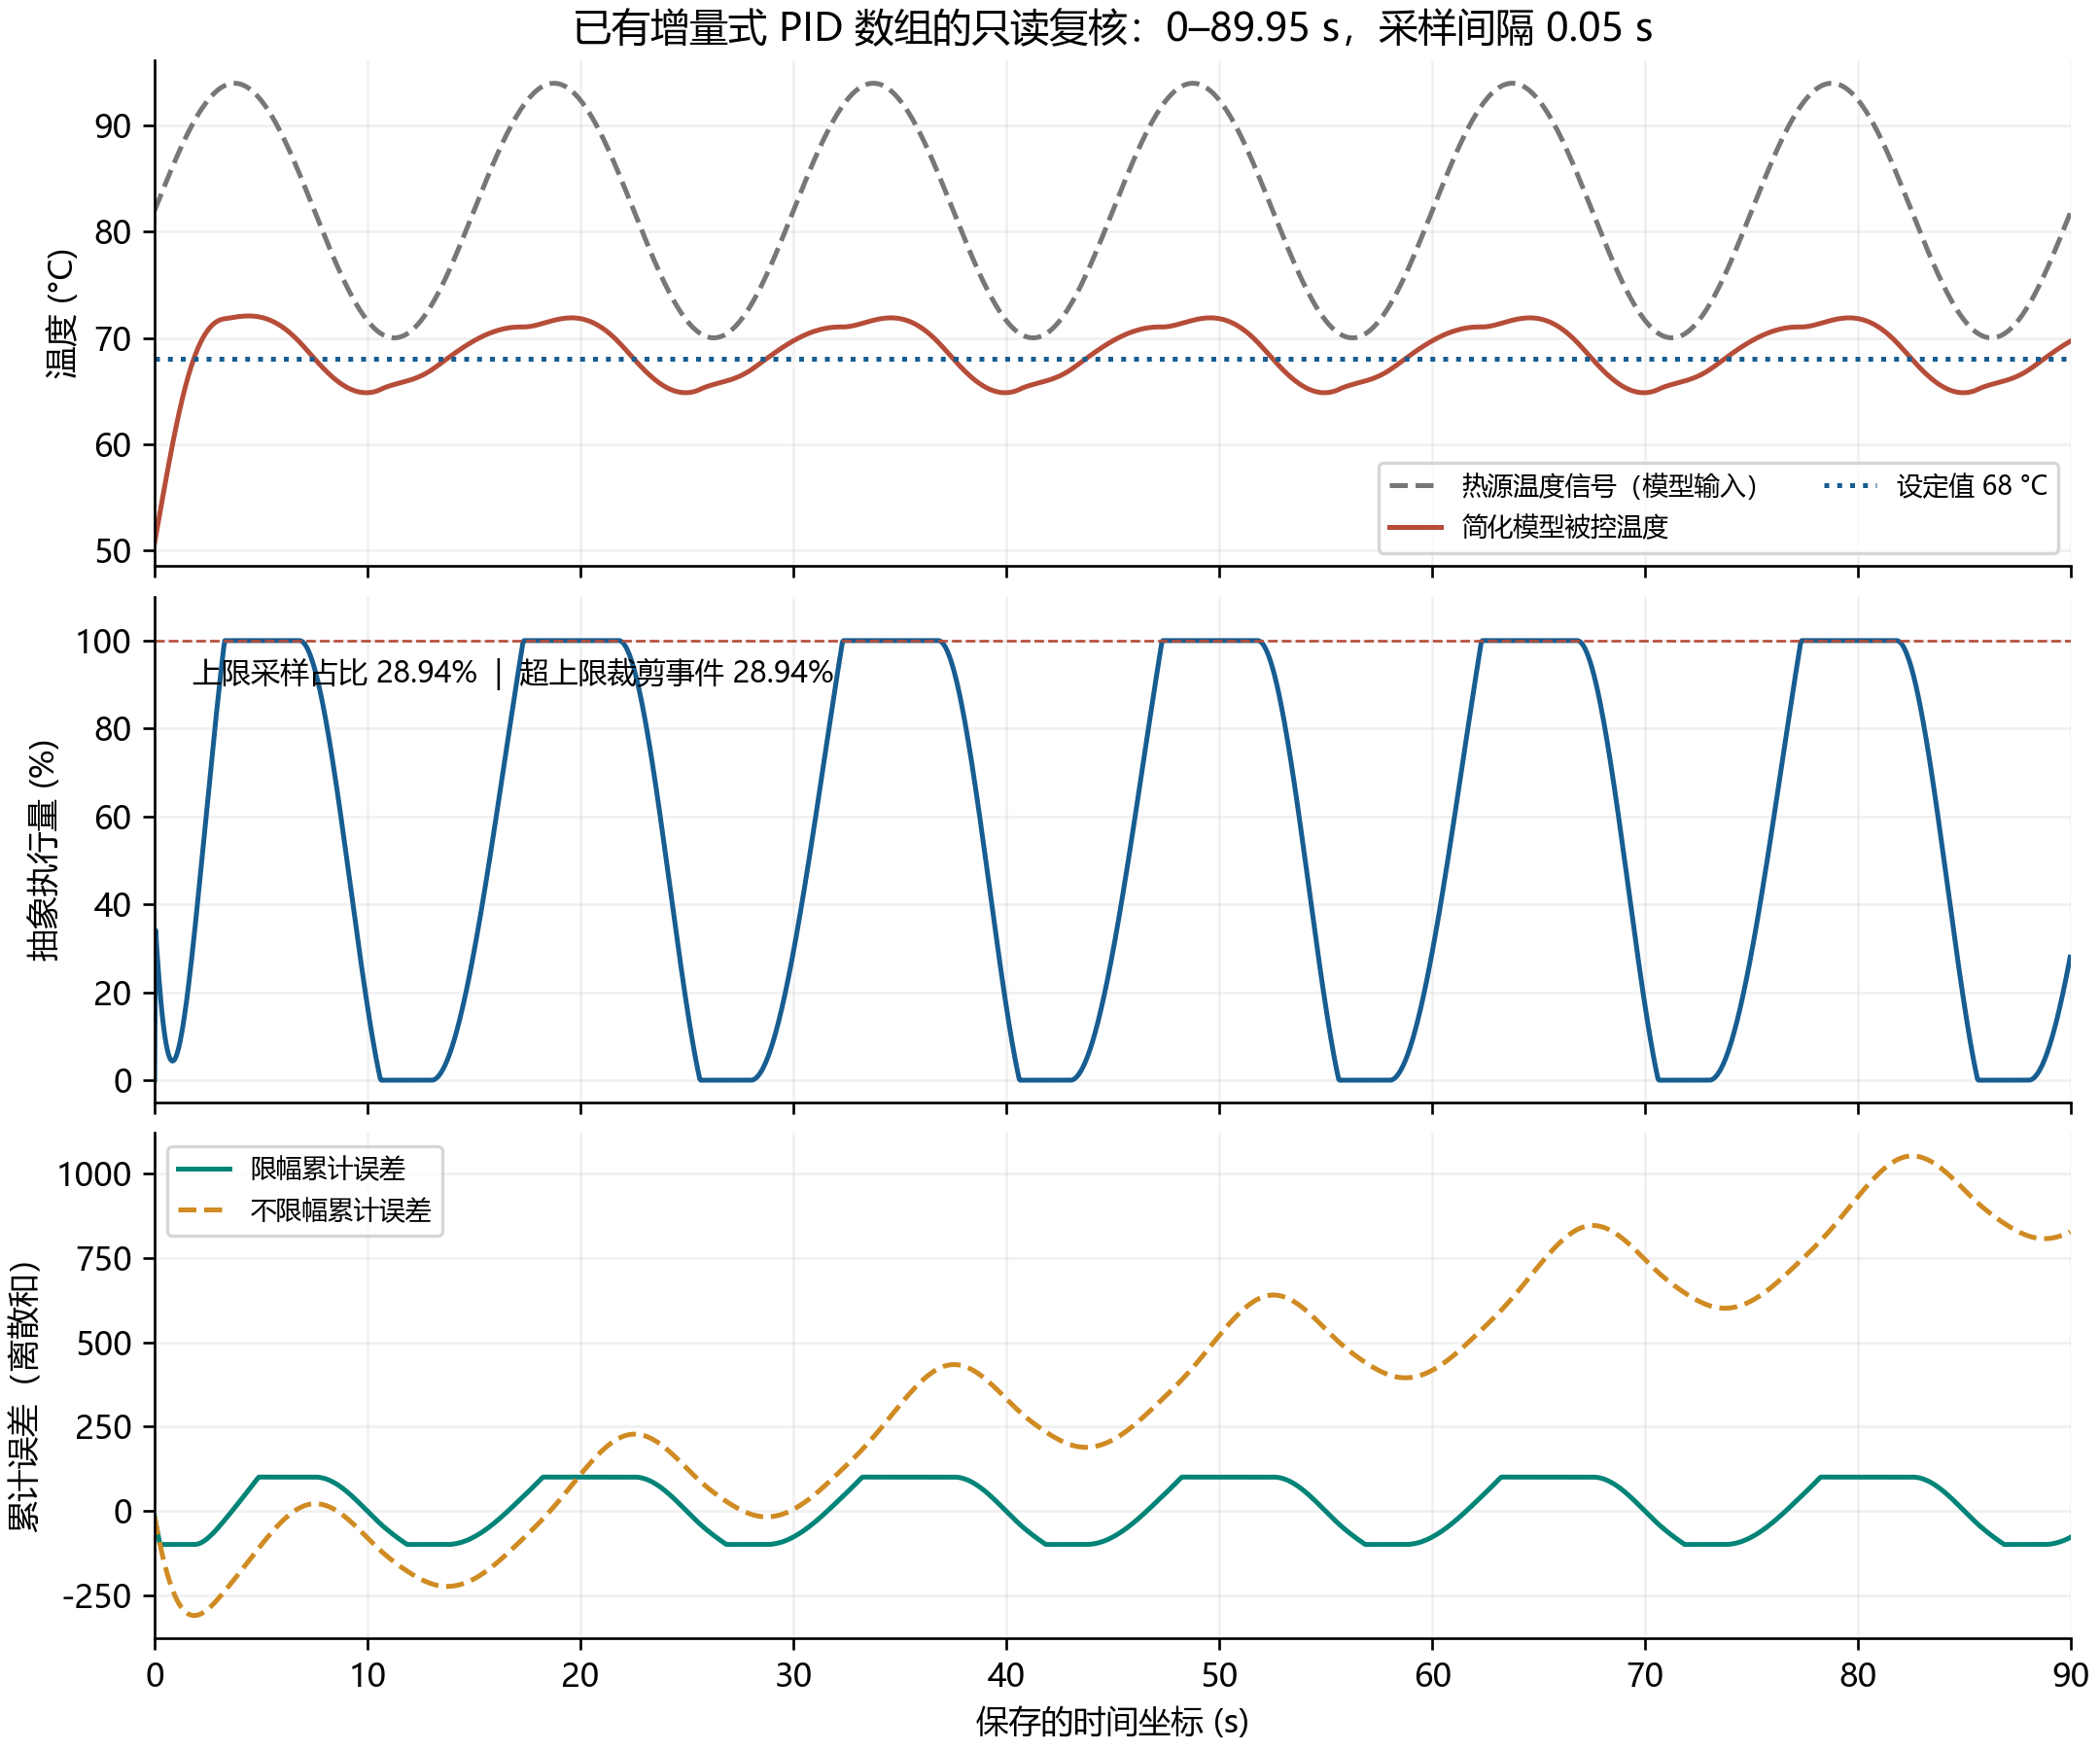
\includegraphics[width=.9\linewidth,height=150mm,keepaspectratio]{../../figs/midterm_asset_pid_verified.png}
\caption{已有简化 PID 温控数组的只读复核。上图为温度扰动与被控温度，中图为限幅执行量，下图为开关累计误差限幅时的累计值；不表示实物流量。}\label{fig:20}
\end{figure}
\clearpage
\setcounter{section}{3}
\setcounter{table}{10}
\begin{table}[!htbp]\centering\small
\caption{保存 PID 时序的工况与复核指标}\label{tab:11}
\begin{tabularx}{\linewidth}{@{}Y Y Y@{}}\toprule
\rowcolor{ydzjlight} 项目 & 数值或状态 & 统计与适用范围 \\\midrule
设定值／初始温度 & 68／50 $^\circ$C & 首个保存温度为更新后50.67625 $^\circ$C。\\
离散增益／采样周期 & $K_p=8.0,K_i=0.5,K_d=2.0$；0.05 s & 增量更新的已有参数，不直接等同连续增益。\\
全时段温度范围 & 50.6763--72.0657 $^\circ$C & 相对68 $^\circ$C全时段最大偏高4.0657 K。\\
后半时段峰值偏高 & 3.8865 K & 原记录3.9 K对应后半段45--89.95 s，不是全程峰值。\\
执行量范围与均值 & 0--100\%；均值54.3705\% & 为经验模型抽象动作，未标定为泵速或流量。\\
上限采样占比 & 28.9444\% & 以保存数组 $U\ge100-10^{-10}$ 逐点统计；原记录29.3\%未由当前数组复现。\\
累计误差峰值 & 限幅100；不限幅1052.6016 & 仅记录累计量变化，不能单独证明抗饱和有效。\\
开关限幅后的温度／执行量差 & 两者最大绝对差均为0 & 当前程序没有将该累计量用于增量更新。\\
\bottomrule\end{tabularx}\end{table}
\clearpage
\setcounter{section}{3}
\setcounter{table}{11}
\begin{table}[!htbp]\centering\small
\caption{按现有保存记录核对的中期任务状态}\label{tab:monthly_status}
\begin{tabularx}{\linewidth}{@{}>{\hsize=0.9\hsize}Y c >{\hsize=1.25\hsize}Y >{\hsize=0.85\hsize}Y@{}}
\toprule
\rowcolor{ydzjlight} 方向与任务 & 状态 & 已有证据 & 下一步 \\
\midrule
方向一：局部结构复现与筛选 & 已有结果 & 三类复现云图；四种流道39工况；六翼型及17条小模型分支。 & 统一工况后进入连接对照。 \\
方向一：连接段及流路集成 & 部分完成 & 连接方案库、40 mm 条带与整板装配几何。 & 连接段成对性能计算。 \\
共享平台：物性实现与数值诊断 & 阶段完成 & 1601点拟合核对、0.137 s实现对照、七档网格与出口诊断。 & 新构型网格与守恒准入。 \\
方向二：动态温控原型 & 部分完成 & 1800点简化 PID 时序及程序复核。 & 抗饱和修正与设备辨识。 \\
方向三：物理融合代理模型 & 部分完成 & 技术路线、数值与自动化资料。 & 样本集与独立测试精度。 \\
系统协同：整板与多行验证 & 未完成 & 已有几何和热源映射。 & 流体域、网格、求解及系统对照。 \\
\bottomrule\end{tabularx}
\par\smallskip\begin{minipage}{\linewidth}\footnotesize 不填完成百分比；简化 PID 结果不代表十行泵阀系统已经验证。\end{minipage}
\end{table}
\clearpage
\setcounter{section}{3}
\setcounter{table}{12}
\begin{table}[!htbp]\centering\small
\caption{已有量化记录与证据边界}\label{tab:key_results}
\begin{tabularx}{\linewidth}{@{}>{\hsize=0.8\hsize}Y >{\hsize=1.1\hsize}Y >{\hsize=1.1\hsize}Y@{}}\toprule
\rowcolor{ydzjlight} 记录 & 量化信息 & 证据边界 \\\midrule
网格敏感性 & 7 档，260169--4610769 单元，统计时刻 0.2 s & 统一以323万档为比较参考；294万档压降差0.3201\%，461万档4.2751\%。\\
温度相关水物性 & 280--360 K，101325 Pa & 拟合适用范围，不表示任意压力与温度均有效。\\
物性实现对照 & 共同 0.137 s 加热面最高温差约 $3.197\times10^{-6}$ K & 实现一致性核对，不代表模型绝对精度。\\
整板几何 & $40\,\mathrm{mm}\times40\,\mathrm{mm}$，$10\times10$ 单元 & 几何与热源映射已完成，整板流热待验证。\\
静态热源布局 & 低/中/高负荷为 70/27/3 格 & 整格加热 2640 W；仅主体加热 2021.25 W。\\
局部模型整理 & 17条代表分支、37条原始提取记录 & 非17种独立结构；各分支工况、物性和时刻分别标识。\\
简化 PID 时序 & 1800点，0.05 s间隔；全程最高72.0657 $^\circ$C & 温度信号扰动；累计误差限幅未接入控制更新。\\
\bottomrule\end{tabularx}\end{table}
\clearpage
\setcounter{section}{4}
\setcounter{table}{0}
\begin{longtable}{>{\centering\arraybackslash}p{0.10\linewidth}>{\centering\arraybackslash}p{0.18\linewidth}>{\centering\arraybackslash}p{0.38\linewidth}>{\centering\arraybackslash}p{0.22\linewidth}}
\caption{下一阶段任务、里程碑与建议分工}\label{tab:16}\\
\toprule
\rowcolor{ydzjlight} 阶段 & 任务 & 可检查交付与判据 & 建议岗位（待确认） \\midrule\\\midrule
\endfirsthead
\multicolumn{4}{l}{表\thetable\ 续：下一阶段研究计划}\\
\toprule
\rowcolor{ydzjlight} 阶段 & 任务 & 可检查交付与判据 & 建议岗位（待确认） \\midrule\\\midrule
\endhead
\midrule\multicolumn{4}{r}{续下页}\\\endfoot
\bottomrule\endlastfoot
M1 & 连接成对计算与归档 & 最终几何、统一工况、成对原始数据、图表与机理说明；— & 成员1主责；成员2复核 \\
M1 & 最小闭环归档 & 热源、反馈、执行器、温度和流量时序；复核最小闭环实际链条 & 成员3主责；成员4复核 \\
M2 & 数值与样本准入 & 参数字典、网格检查、物性、守恒与收敛标签；— & 成员2主责；成员1复核 \\
M2 & 物理动态模型辨识 & 热阻热容及水力网络、参数辨识与独立动态响应；— & 成员3主责；成员2支撑 \\
M3 & 基础与物理融合模型 & 统一划分、基础算法、融合与消融、样本效率和泛化测试 & 成员4主责；成员2支撑 \\
M3 & 控制算法比较 & 同扰动/初态/约束；温度、均匀性、动作与能量统计 & 成员3主责；成员1支撑 \\
M4 & 系统级协同验证 & 同一整板对象的参考CFD、动态场景、误差与成本评价；— & 四人共同；负责人统筹 \\
M4 & 报告与成果整理 & 来源索引、图表定稿、阶段性论文稿及报告终审；不预设发表 & 四人共同；指导教师审核 \\
\end{longtable}
\clearpage
\setcounter{section}{4}
\setcounter{figure}{0}
\reportfigure{fig:30}{下一阶段总体路线与里程碑}{../../figs/midterm_concept_fig_30.pdf}{\linewidth}
\clearpage
\setcounter{section}{4}
\setcounter{table}{1}
\begin{table}[!htbp]\centering\small
\caption{连接与整板的验证项目、指标及缺口}\label{tab:system_checks}
\begin{tabularx}{\linewidth}{@{}Y Y Y@{}}\toprule
\rowcolor{ydzjlight} 验证内容 & 统一评价方式 & 当前输入与待补证据 \\\midrule
分区是否有效 & 同受热面最高温、极差、面积标准差 & 已有70/27/3几何映射；需整板温度场及均匀布置基准。\\
流动分配是否合理 & 支路流量偏差、入口均匀性、连接压降占比 & 已有连接几何；需各行流量和连接前后截面数据。\\
能效是否可接受 & 相同热源与约束下的水力功、必要时电功 & 需系统压差、体积流量与设备效率；不由局部压降直接推电耗。\\
是否优于单一流道 & 同整板尺寸、负荷与泵功下比较 & 单元数据已有，整板独立基准与复合方案均需计算。\\
控制是否可落地 & 执行器至流量、流量／水温至反馈温度的独立辨识 & 简化 PID 时序已有；实际泵阀特性、采样与多行响应待补。\\
\bottomrule\end{tabularx}\end{table}
\clearpage
\begin{thebibliography}{99}
\bibitem{stagereports} 项目组. 阶段研究报告汇编及配套图表（内部资料）[R]. 2026. 采用本次整理时保存的版本。
\bibitem{tuckerman1981} Tuckerman D B, Pease R F W. High-performance heat sinking for VLSI[J]. IEEE Electron Device Letters, 1981, 2(5): 126--129. DOI: 10.1109/EDL.1981.25367.
\bibitem{ref16} 王雅博, 诸凯, 崔卓, 等. 冷却水进出方式对芯片散热器换热性能影响[J]. 机械工程学报, 2018, 54(10): 188--194.
\bibitem{ref17} Choi W W, Bang S H, Shin H C, et al. Experimental and numerical study of a high-performance air-cooled N-type manifold microchannel heat sink for large-area applications[J]. International Communications in Heat and Mass Transfer, 2026, 175: 110986.
\bibitem{ref6} 张乾坤, 李红艳, 吕碧纯, 等. 叶脉仿生微通道换热器流动与传热特性的数值研究[J]. 制冷学报, 2025, 46(4): 52--60.
\bibitem{ref5} Wang M, Xie J, Bu J, et al. Thermo-hydraulic effects of asymmetric-height and fractal bifurcation channels combined with impingement in microchannel heat sinks[J]. Applied Thermal Engineering, 2026, 298: 130998.
\bibitem{ref7} Yang G, Tang Y, Sun Y, et al. Fabrication of microchannel heat sinks using additive manufacturing: A review[J]. Renewable and Sustainable Energy Reviews, 2026, 233: 116879.
\bibitem{ref13} Ansari D, Kim K Y. Hotspot thermal management using a microchannel-pinfin hybrid heat sink[J]. International Journal of Thermal Sciences, 2018, 134: 27--39.
\bibitem{ref24} Lorenzini D, Green C, Sarvey T E, et al. Embedded single phase microfluidic thermal management for non-uniform heating and hotspots using microgaps with variable pin fin clustering[J]. International Journal of Heat and Mass Transfer, 2016, 103: 1359--1370.
\bibitem{ref2} Xu H, Wang Y, Tian W, et al. Thermal performance optimization of dual-bridge arm SiC IGBT modules via microstructure-modified microchannel heat sinks under double-sided liquid cooling[J]. International Communications in Heat and Mass Transfer, 2026, 176: 111339.
\bibitem{ji} 季俊杰. 微通道冷却芯片及其热点的动态特性研究[D]. 杭州: 浙江大学, 2021.
\bibitem{wu} 吴睿康. 电子器件主动液冷散热的建模及实验研究[D]. 杭州: 浙江大学, 2020.
\bibitem{laguna} Laguna G, Vilarrubi M, Ibanez M, et al. Numerical parametric study of a hotspot-targeted microfluidic cooling array for microelectronics[J]. Applied Thermal Engineering, 2018, 144: 71--80.
\bibitem{hushousong} 胡寿松. 自动控制原理[M]. 8 版. 北京: 科学出版社, 2023.
\bibitem{astrom} {\AA}strom K J, H{\"a}gglund T. PID Controllers: Theory, Design, and Tuning[M]. 2nd ed. Research Triangle Park: Instrument Society of America, 1995.
\bibitem{ogata} Ogata K. Modern Control Engineering[M]. 5th ed. Upper Saddle River: Prentice Hall, 2010.
\bibitem{tao} Tao F, Zhang H, Zhang C. Advancements and challenges of digital twins in industry[J]. Nature Computational Science, 2024, 4(3): 169--177.
\bibitem{brunton} Brunton S L, Kutz J N. Data-Driven Science and Engineering: Machine Learning, Dynamical Systems, and Control[M]. 2nd ed. Cambridge: Cambridge University Press, 2022.
\bibitem{chen2016} Chen T, Guestrin C. XGBoost: A Scalable Tree Boosting System[EB/OL]. arXiv:1603.02754, 2016. DOI: 10.48550/arXiv.1603.02754. 预印本；用于基础算法来源。
\bibitem{raissi2017} Raissi M, Perdikaris P, Karniadakis G E. Physics Informed Deep Learning (Part I): Data-driven Solutions of Nonlinear Partial Differential Equations[EB/OL]. arXiv:1711.10561, 2017. DOI: 10.48550/arXiv.1711.10561. 预印本；用于物理约束学习的方法背景。
\end{thebibliography}
\end{document}
